\chapter{Estructura del Contenido}

\section{Arquitectura}

El proyecto cuenta con tres módulos principales, cuyos componentes son parte exclusiva de uno de los módulos o, en caso del servidor Flask, de todos ellos. Este servidor funciona como puente y permite la unificación de los 3 módulos en un único sistema. Un factor decisivo a la hora de elegir esta arquitectura fue la seguridad de la red MQTT.

Añadir seguridad en redes de IOT es un tema complejo dada la naturaleza limitada de las redes y dispositivos que las integran. El costo de overhead y procesamiento inherente a la seguridad en el intercambio de mensajes entre broker y los nodos puede ser mayor al beneficio obtenido. Es por esto que se debe analizar alternativas al uso de SSL/TLS de los que se habló anteriormente.

Si el diseño de la arquitectura de la red MQTT es malo y, además, no se utiliza SSL/TLS, es decir, los mensajes se mandan en texto plano, es muy simple que un hacker inyecte mensajes en la red.~\cite{SecurityInTheIoT} Por ejemplo, si el broker estuviera conectado a los nodos en una red wifi abierta, un hacker podría conectarse a la red, sniffear los mensajes, ver el formato de los mensajes entre broker y nodos logrando así entender que topics y payloads se utilizan para realizar ciertas acciones como prender y apagar el relé y publicar el las acciones en vez del broker. A través de este ejemplo es fácil darse cuenta es extremadamente importante tener una  contraseña para la red MQTT y con un nivel de seguridad alto como WPA/WPA2, para que sea computacionalmente difícil de que un hacker se conecte a la red e infecte mensajes.~\cite{WiFiSecurity} 

Otro posible problema es que la red MQTT sea la misma que la red de la persona, lo que puede dar lugar a que si esta persona no tiene una buena contraseña en su red, esté expuesta a que un hacker pueda conectarse a la red utilizando contraseñas populares o que una persona que se haya conectado alguna vez tenga luego malas intenciones.

Para mejorar las arquitecturas de seguridad mencionadas anteriormente se propone:

\begin{itemize}

\item Tener 4 contraseñas involucradas en arquitectura: 
	
	\begin{enumerate}
	\item La que se debe crear el usuario para registrarse en la base de datos mongo y así tener acceso a las funciones de sistema como el apagado y prendido de los relé. Esta autenticación hace que no cualquier persona en la red local del hogar pueda tener acceso a esas funciones, solo los que se autentifican. 

	\item La segunda contraseña es la de la red local de la casa a la cual se debe conectar el Raspberry Pi luego de la instalación inicial.

	\item La tercera es la de la red MQTT. Esta red tendrá un nombre y contraseña luego de la instalación del sistema de la cual el usuario nunca se deberá preocupar, será transparente para el mismo. Esta contraseña es elegida con una combinación entre la MAC del Raspberry Pi donde se alberga el broker y la hora a la que se crea la misma. Todos los nodos que se conecten tendrán que guardar esa contraseña en sus SPIFFS y adquirirla de ahí al prenderse para conectarse.

	\item La última contraseña es con la que se comunican entre los nodos entre ellos cuando alguno no llega a recibir la señal del broker. Está contraseña también debe ser única y crearse con un criterio similar a la de la red MQTT. Esta contraseña permite que si dos clientes independientes instalarán el producto en lugares cercanos, los mensajes de uno y otro no se mezclen. De la misma manera, un hacker tampoco podría ingresar mensajes a la red usando nodos con el software del sistema.

\end{enumerate}

\item Como se puede ver en la figura~\qref{fig:redes-sep}, se hace una separación tanto física como lógica de la red MQTT con la red del usuario. Una está dedicada a la red MQTT y otra es la red local del usuario que manda las órdenes al Flask y este traduce a órdenes MQTT. Esta arquitectura resuelve los problemas expuestos anteriormente dado que se tiene control sobre la red MQTT. Esta red es transparente para el usuario y esto permite que se puedan crear una contraseña \lstinline[columns=fixed]{WPA/WPA2} muy segura utilizando la dirección \lstinline[columns=fixed]{MAC} del dispositivo y la hora de creación de la misma, como se explicó anteriormente.
Crear una red MQTT separada de la red del usuario no solo mejora la seguridad. Mientras menos se dependa de una red local donde personas ajenas al proyecto pueden cambiar su configuración, mayor control se tiene sobre el ambiente en el que corre el sistema. 

\afterpage{
\begin{figure}[H]
  \centering
  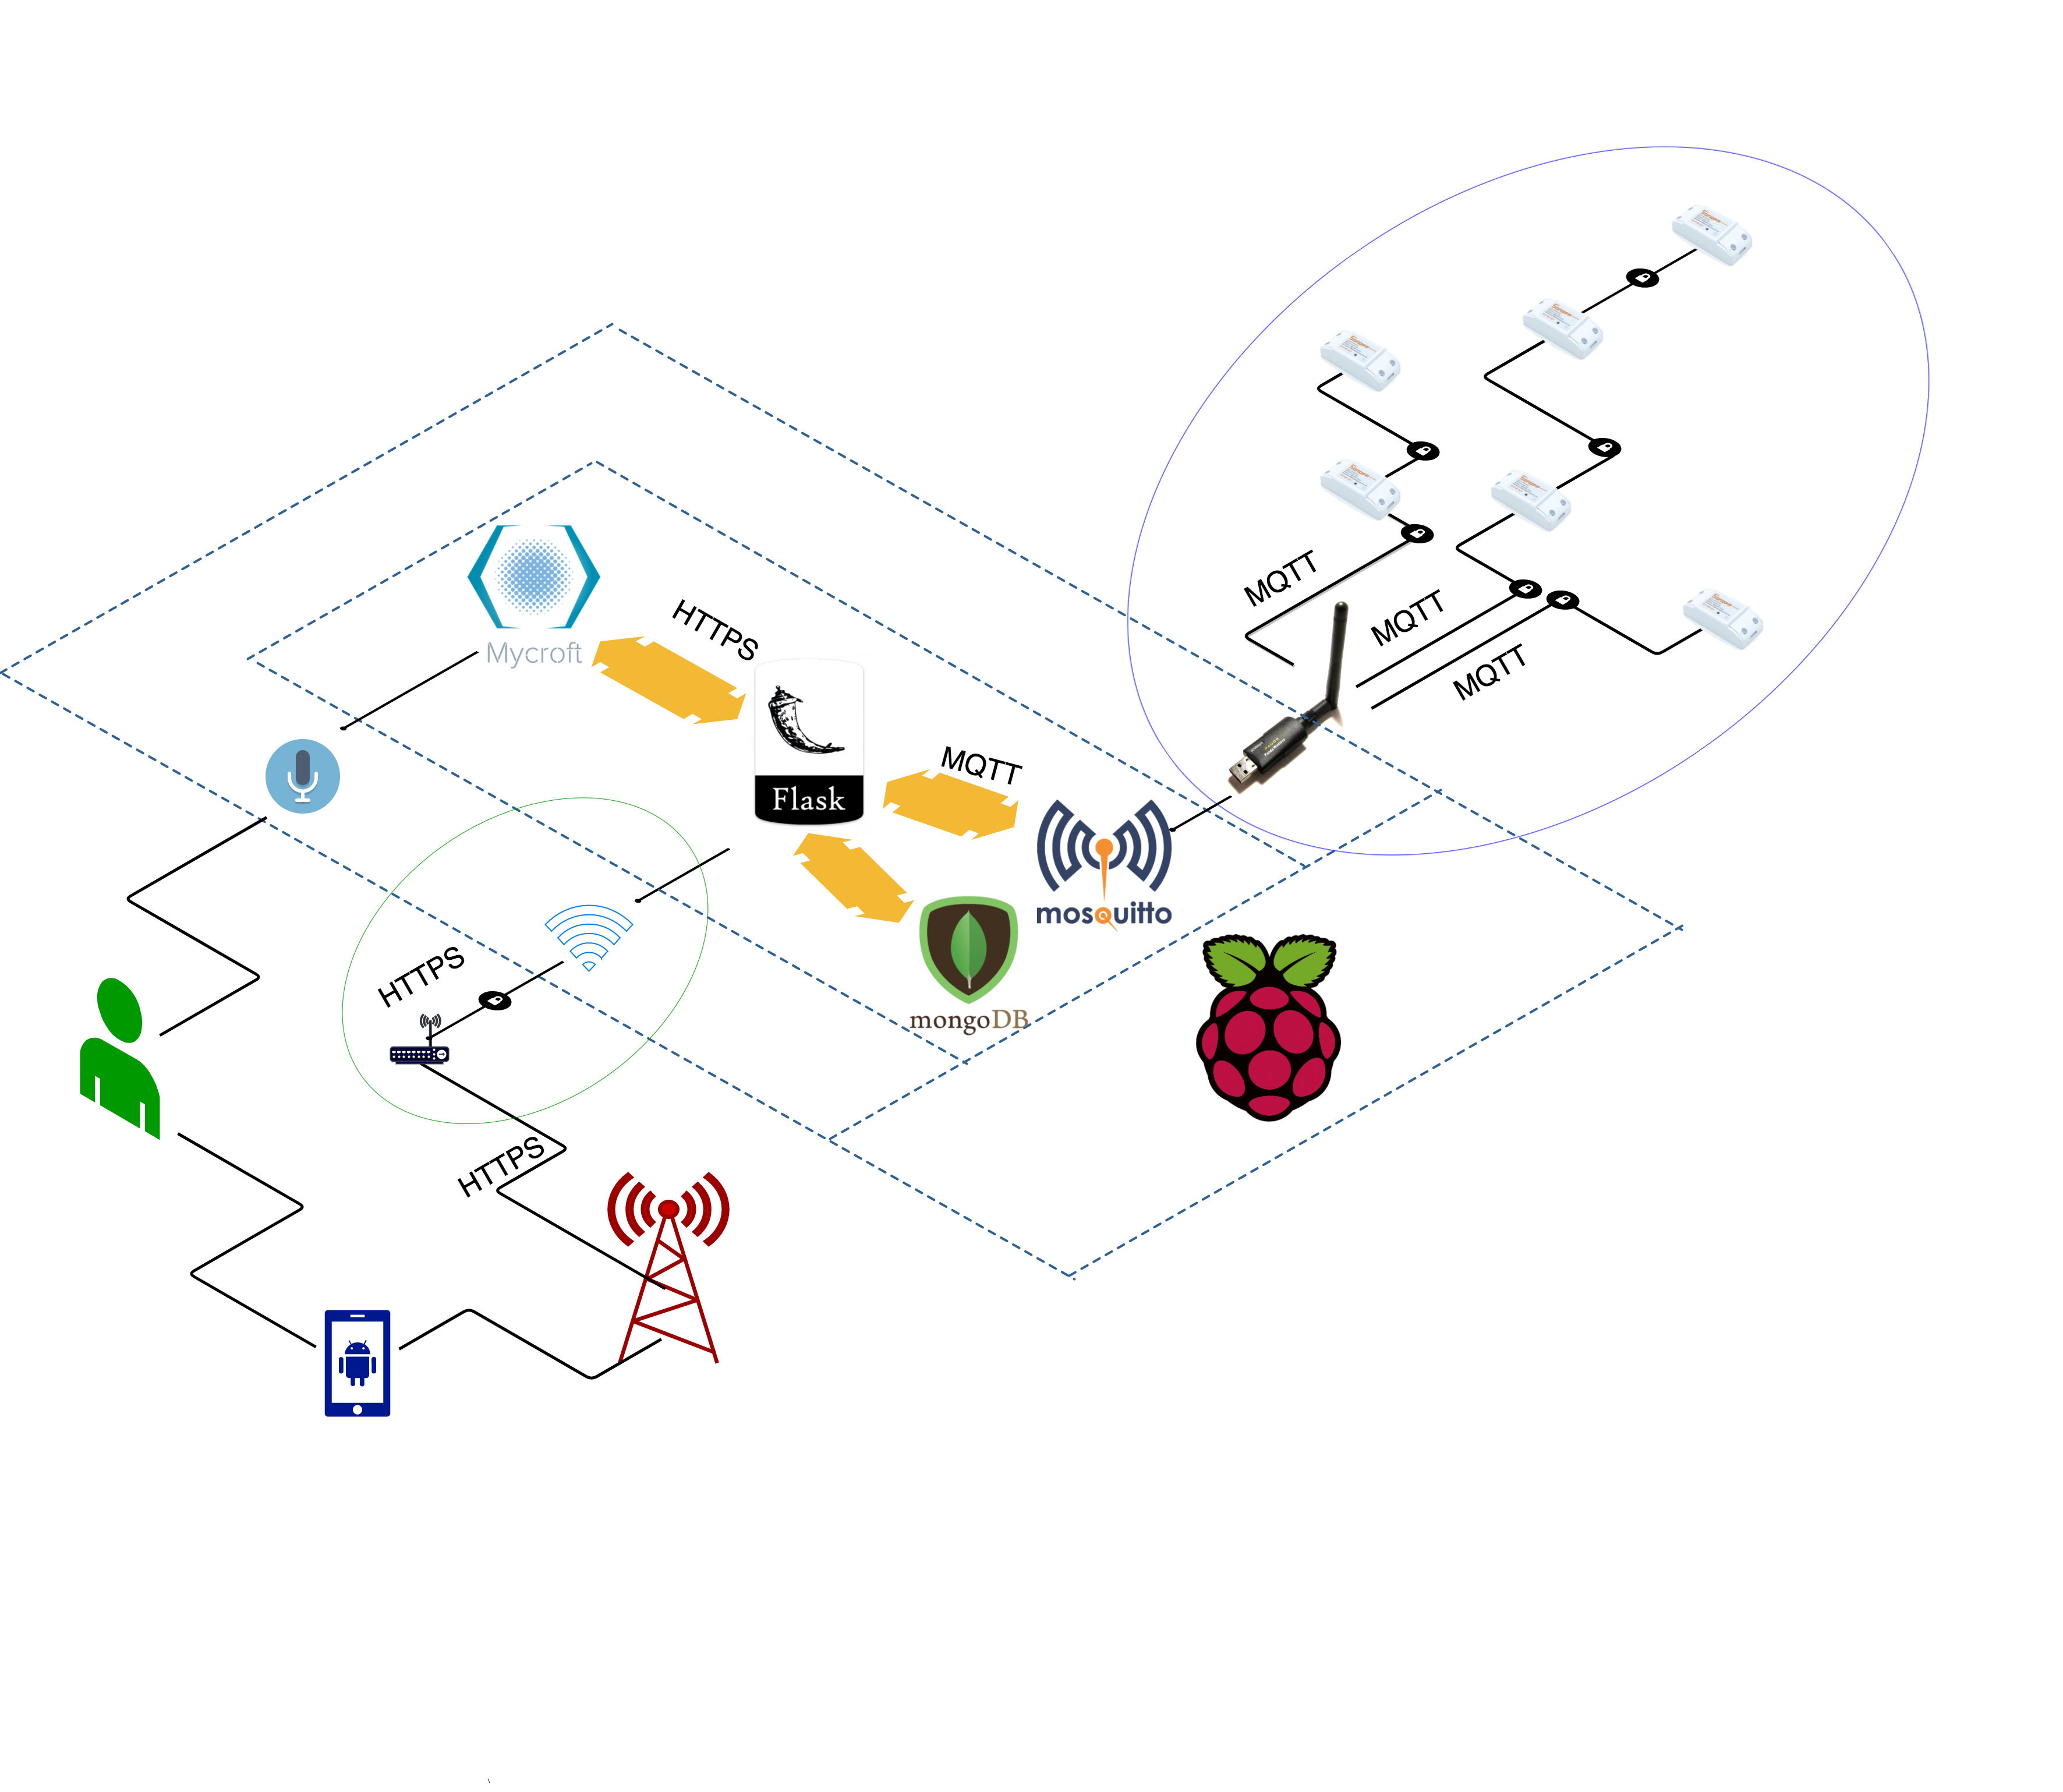
\includegraphics[width=0.6\textwidth, keepaspectratio]{images/redes-separadas}
  \caption{\textit{Redes en el sistema.}}
  \label{fig:redes-sep}

\end{figure}
\clearpage
}

\end{itemize}


\section{Módulos del Sistema}

\subsection{Módulo MQTT Mesh}

\subsubsection{Componentes:} ~\qref{fig:mod-mqtt-comp}

\begin{itemize}

\item Interruptores Sonoff

\item Raspberry Pi: Específicamente el access point configurado en el dongle Panda, el broker Mosquitto y el servidor Flask.

\end{itemize}

\begin{figure}[h]
  \centering
  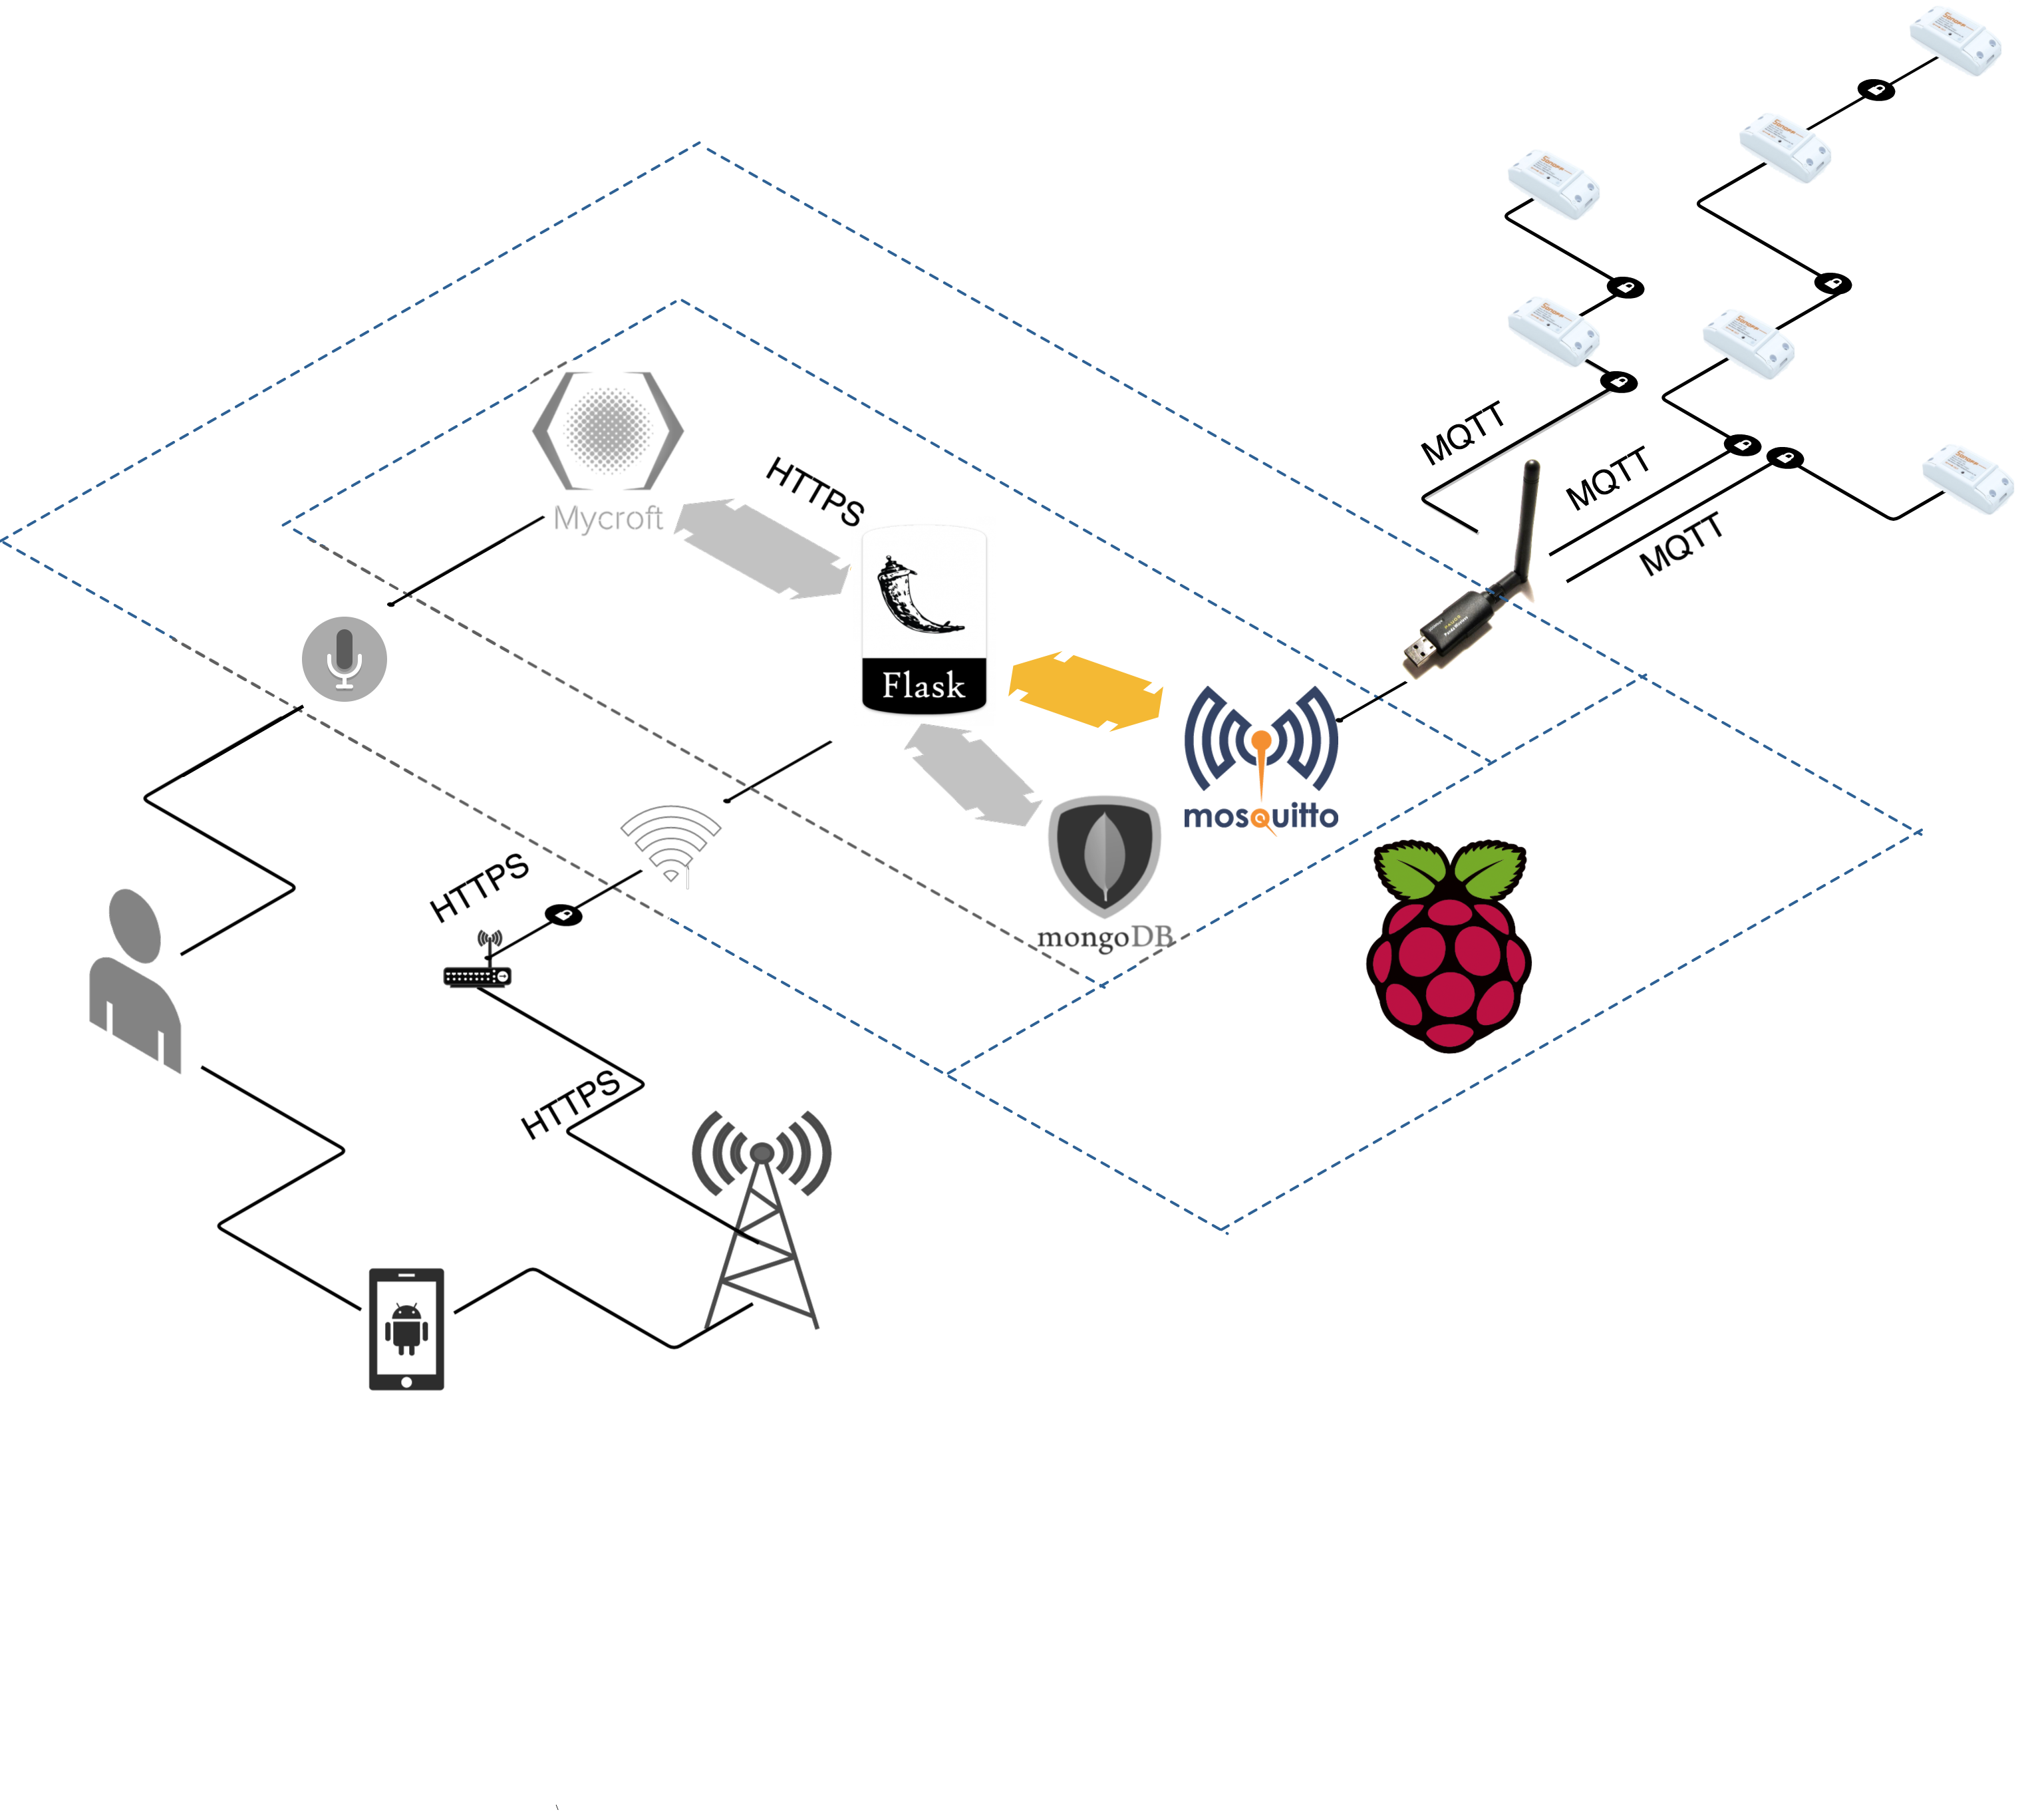
\includegraphics[width=0.6\textwidth, keepaspectratio]{images/mod-MQTT}
  \caption{\textit{Componentes del Módulo MQTT Mesh.}}
  \label{fig:mod-mqtt-comp}
\end{figure}

\subsubsection{Descripción:}

Este módulo es la base del sistema y su funcionamiento es el siguiente:

\begin{itemize}

\item El broker Mosquitto se encarga de la distribución de los mensajes MQTT a los componentes conectados al Raspberry Pi por el Access-Point configurado con el dongle.

\item El software en los interruptores sonoff permiten la conexión al broker directamente o a través de otro interruptor perteneciente a la misma red. Estos dispositivos son configurables a través de la aplicación web, permitiendo así configurar tanto el nombre como contraseña de la red.

\item El servidor Flask se suscribe y publica en topics, siendo el único componente de la red además de los interruptores inteligentes.

\end{itemize}


\subsection{Módulo de Control}

\subsubsection{Componentes:} ~\qref{fig:mod-ctrl-comp}

\begin{itemize}

\item Raspberry Pi: Específicamente la base de datos MongoDB y el servidor Flask.

\end{itemize}

\begin{figure}[h]
  \centering
  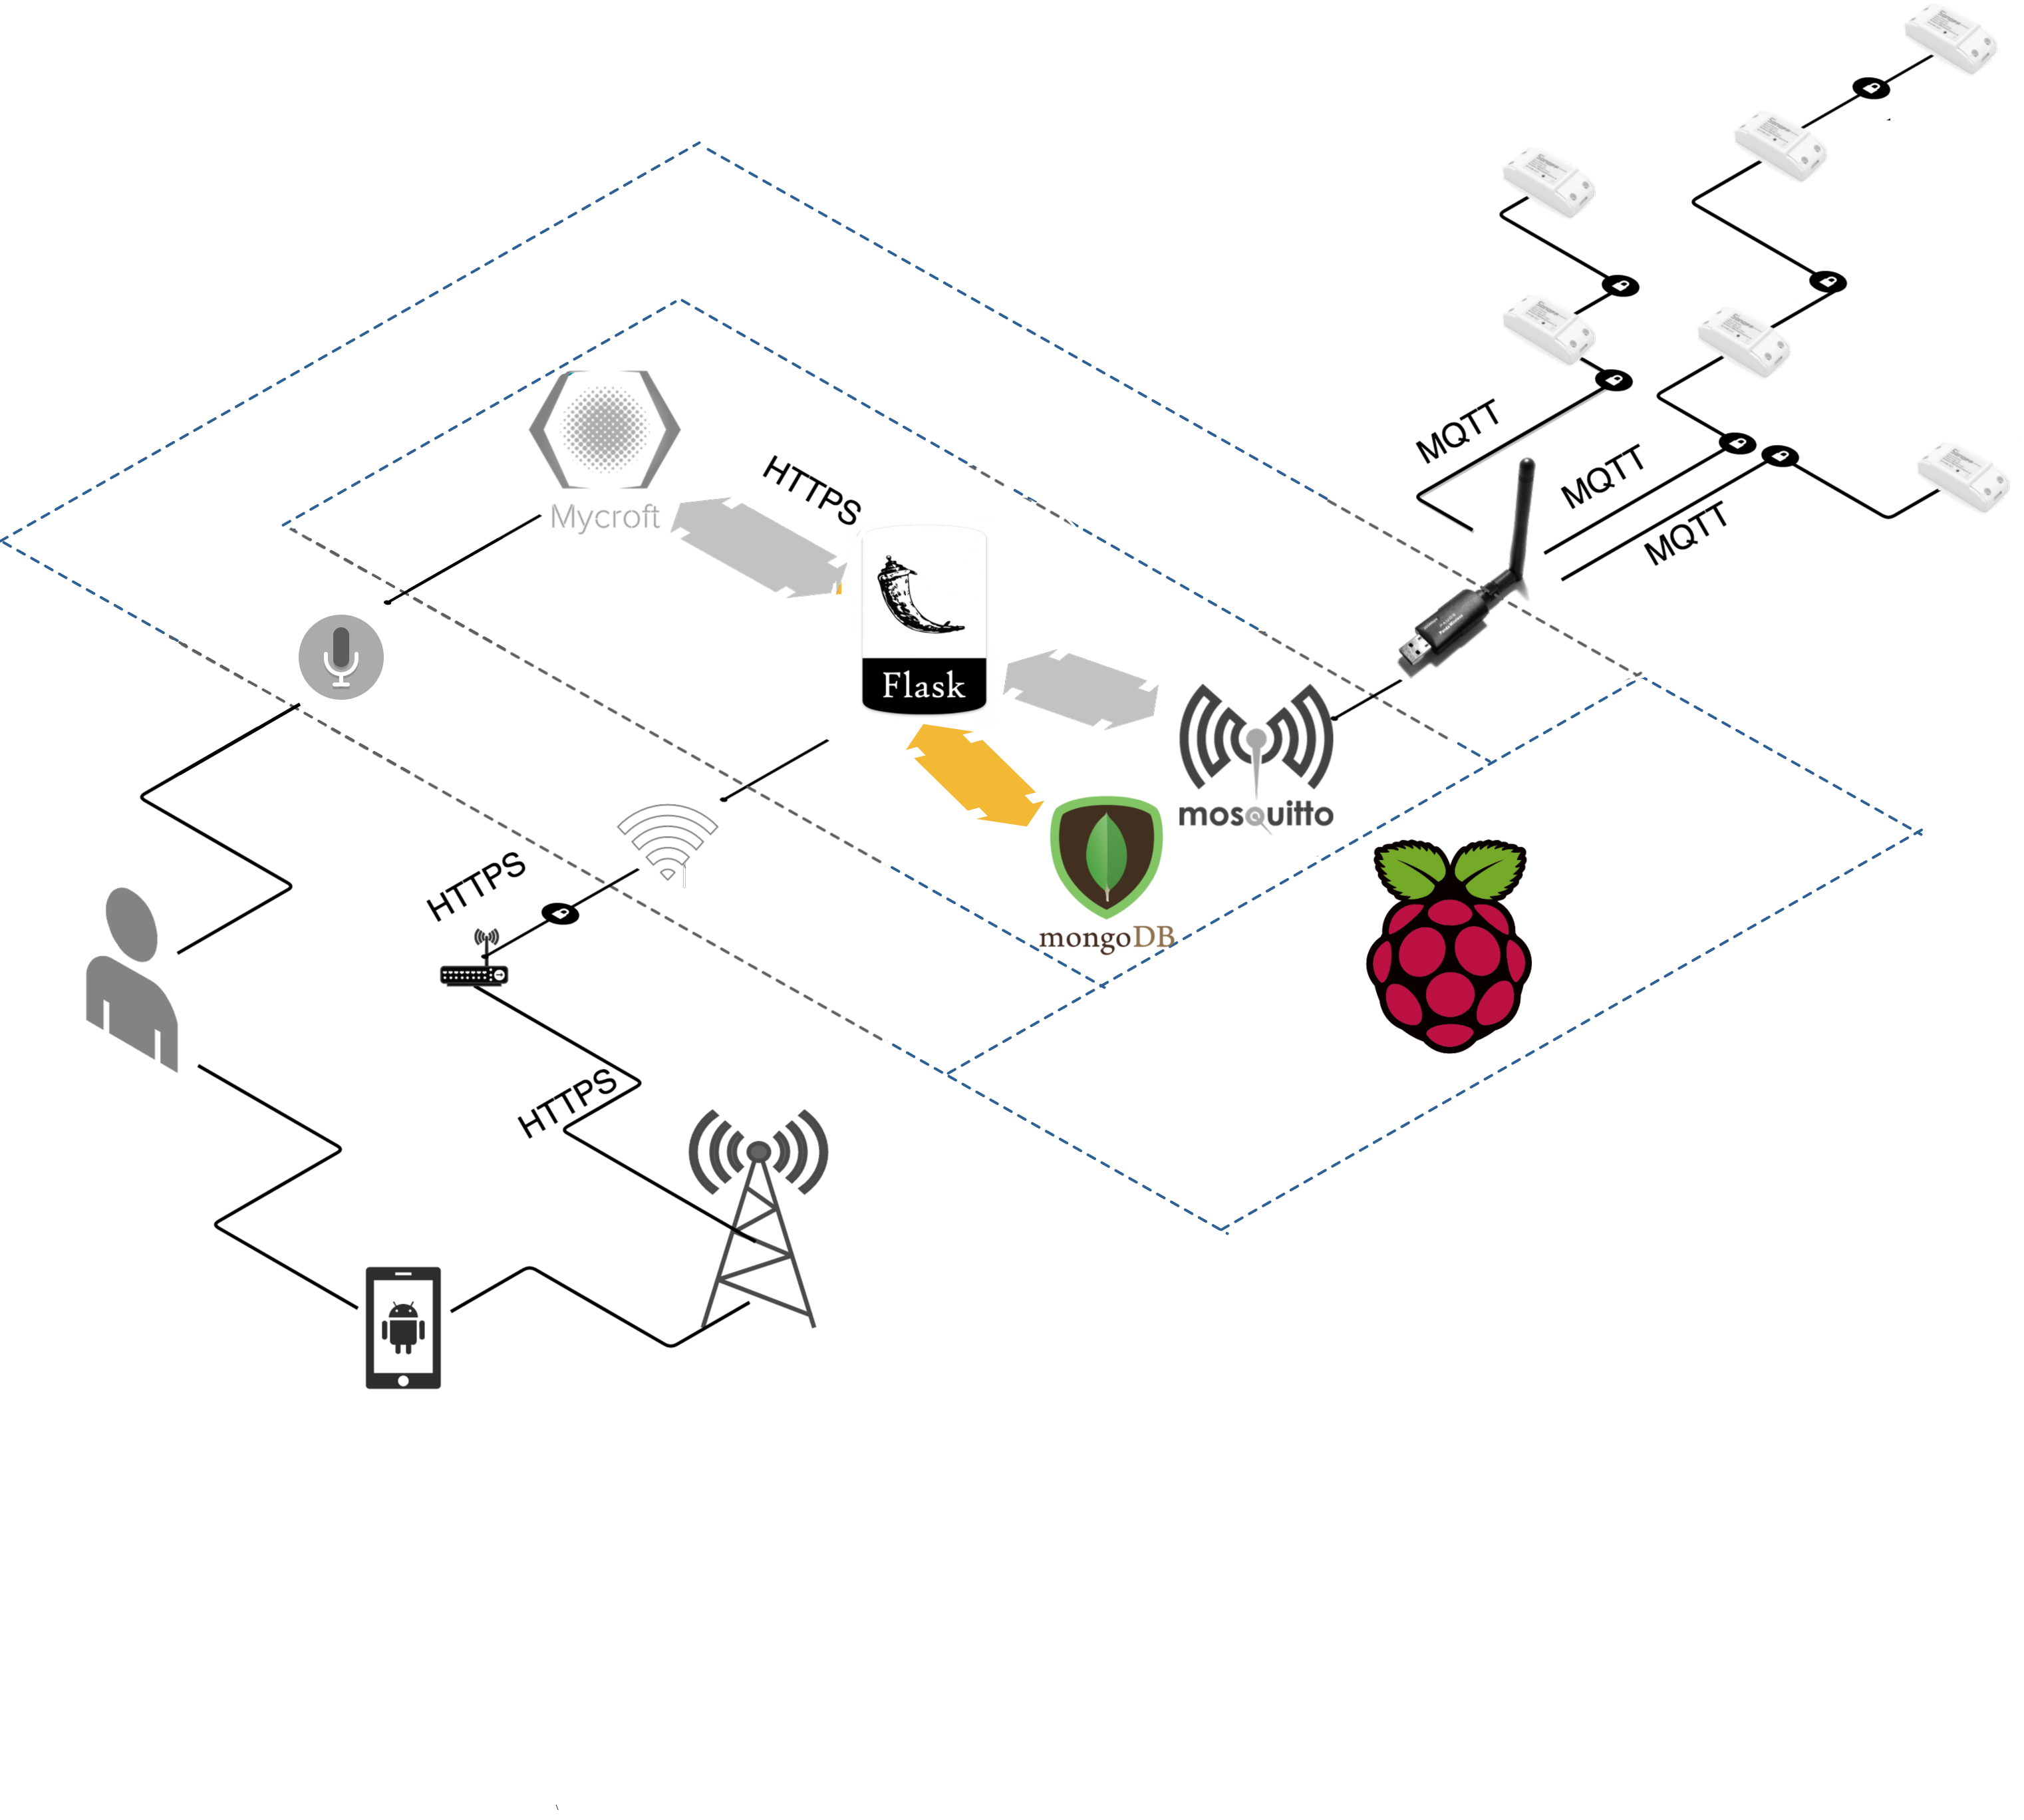
\includegraphics[width=0.6\textwidth, keepaspectratio]{images/mod-ctrl}
  \caption{\textit{Componentes del Módulo de Control.}}
  \label{fig:mod-ctrl-comp}
\end{figure}

\subsubsection{Descripción:}

El servidor Flask se conecta a la red MQTT, permitiendo así suscribirse y publicar en distintos topics. Este servidor será accesible por las interfaces de usuario como único punto de acceso a los componentes de la red MQTT, se encargará de traducir los mensajes enviados por estas interfaces y de manejar otras estructuras de datos necesarias para la interacción con los componentes. Llevará un registro en la MongoDB de todos los componentes conectados al broker, junto con los topics para poder interactuar con ellos y a los demás datos de cada componente, así como nombre, habitación o grupo al que pertenecen.

\subsection{Módulo de interfaces de usuario}

\subsubsection{Aplicación web}

\paragraph{Componentes:} ~\qref{fig:mod-ui-webapp}

\begin{itemize}

\item Aplicación contenida en el dispositivo móvil.

\end{itemize}

\begin{figure}[h]
  \centering
  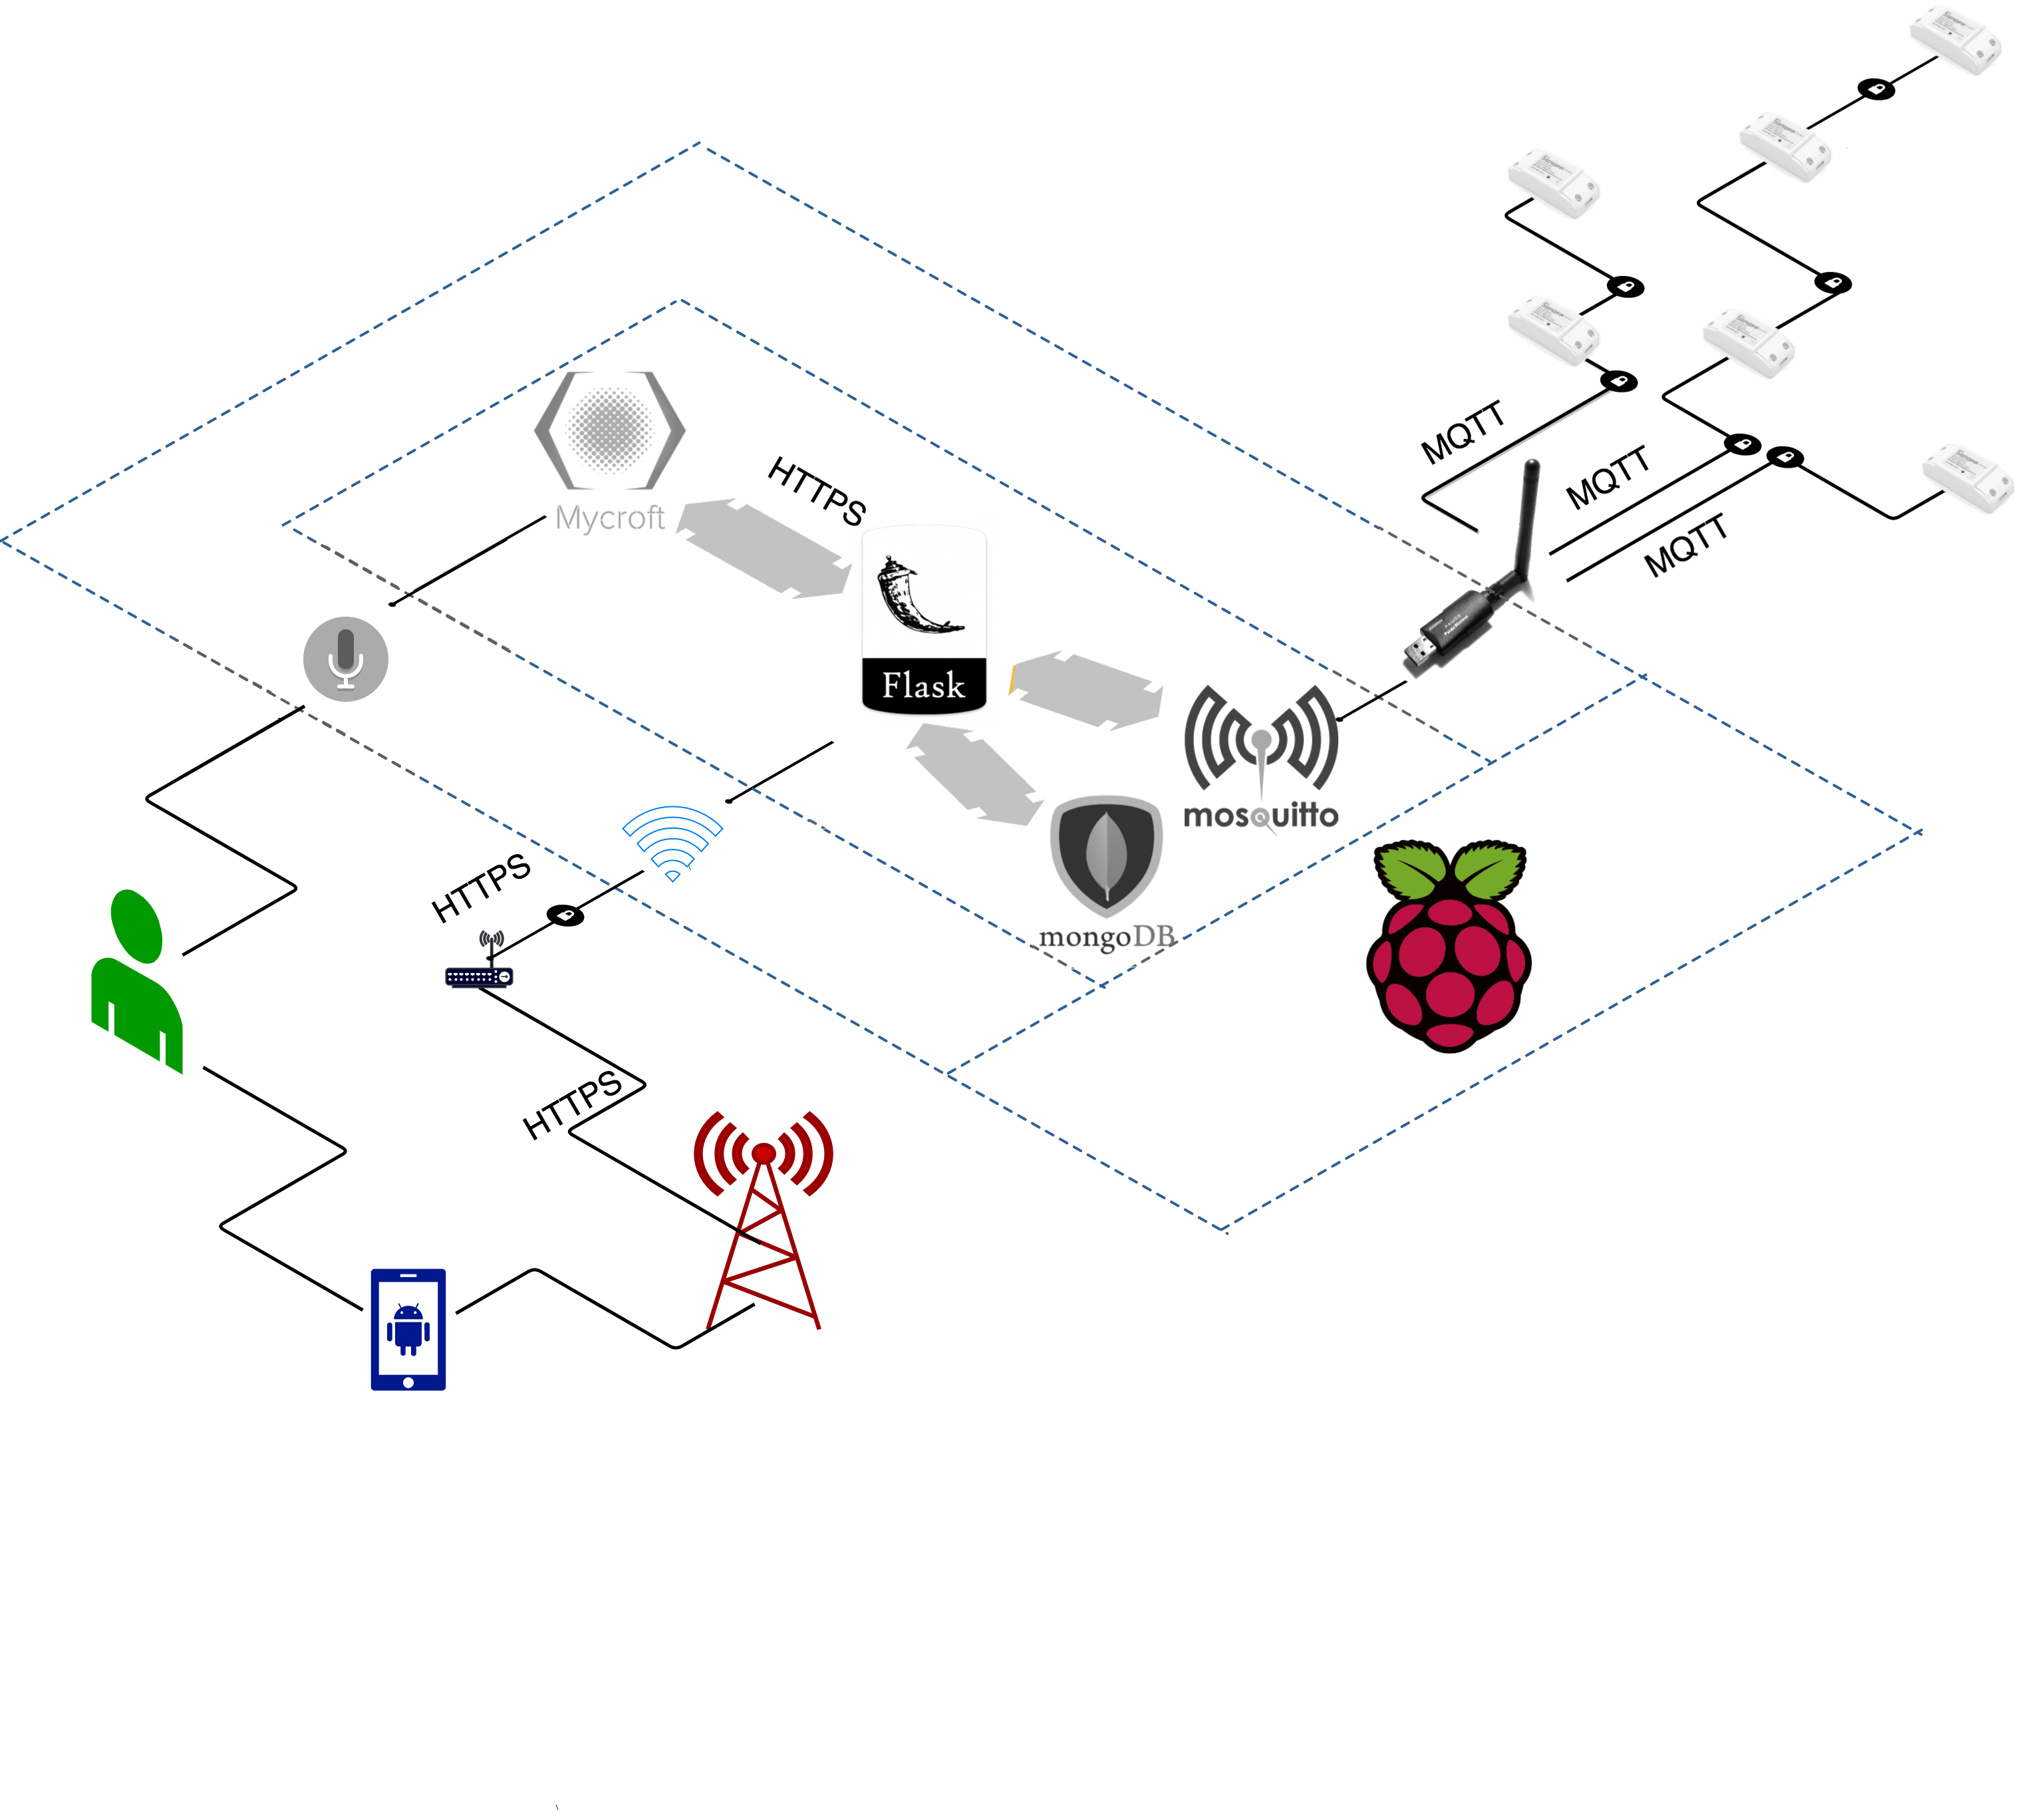
\includegraphics[width=0.6\textwidth, keepaspectratio]{images/mod-ui-webapp}
  \caption{\textit{Componentes del Módulo de UI para Aplicación Móvil.}}
  \label{fig:mod-ui-webapp}
\end{figure}

\paragraph{Descripción:}

\begin{itemize}

\item Esta aplicación permite interactuar de una manera sencilla e intuitiva con los servicios proveídos por los módulos anteriormente mencionados.

\item Una de las funciones básicas es conectarse a los interruptores inalámbricos en modo configuración, y así modificar las credenciales necesarias para acceder a la red proveída por el Raspberry Pi.

\item También expone los dispositivos pertenecientes a la red, permitiendo apagar, prender y programar una de las anteriores acciones para un momento determinado.

\end{itemize}


\subsubsection{Asistente virtual}

\paragraph{Componentes:} ~\qref{fig:mod-ui-mycroft}

\begin{itemize}

\item Asistente Mycroft, localizado en Raspberry Pi.

\item Micrófono, conectado al Raspberry Pi.

\end{itemize}

\begin{figure}[h]
  \centering
  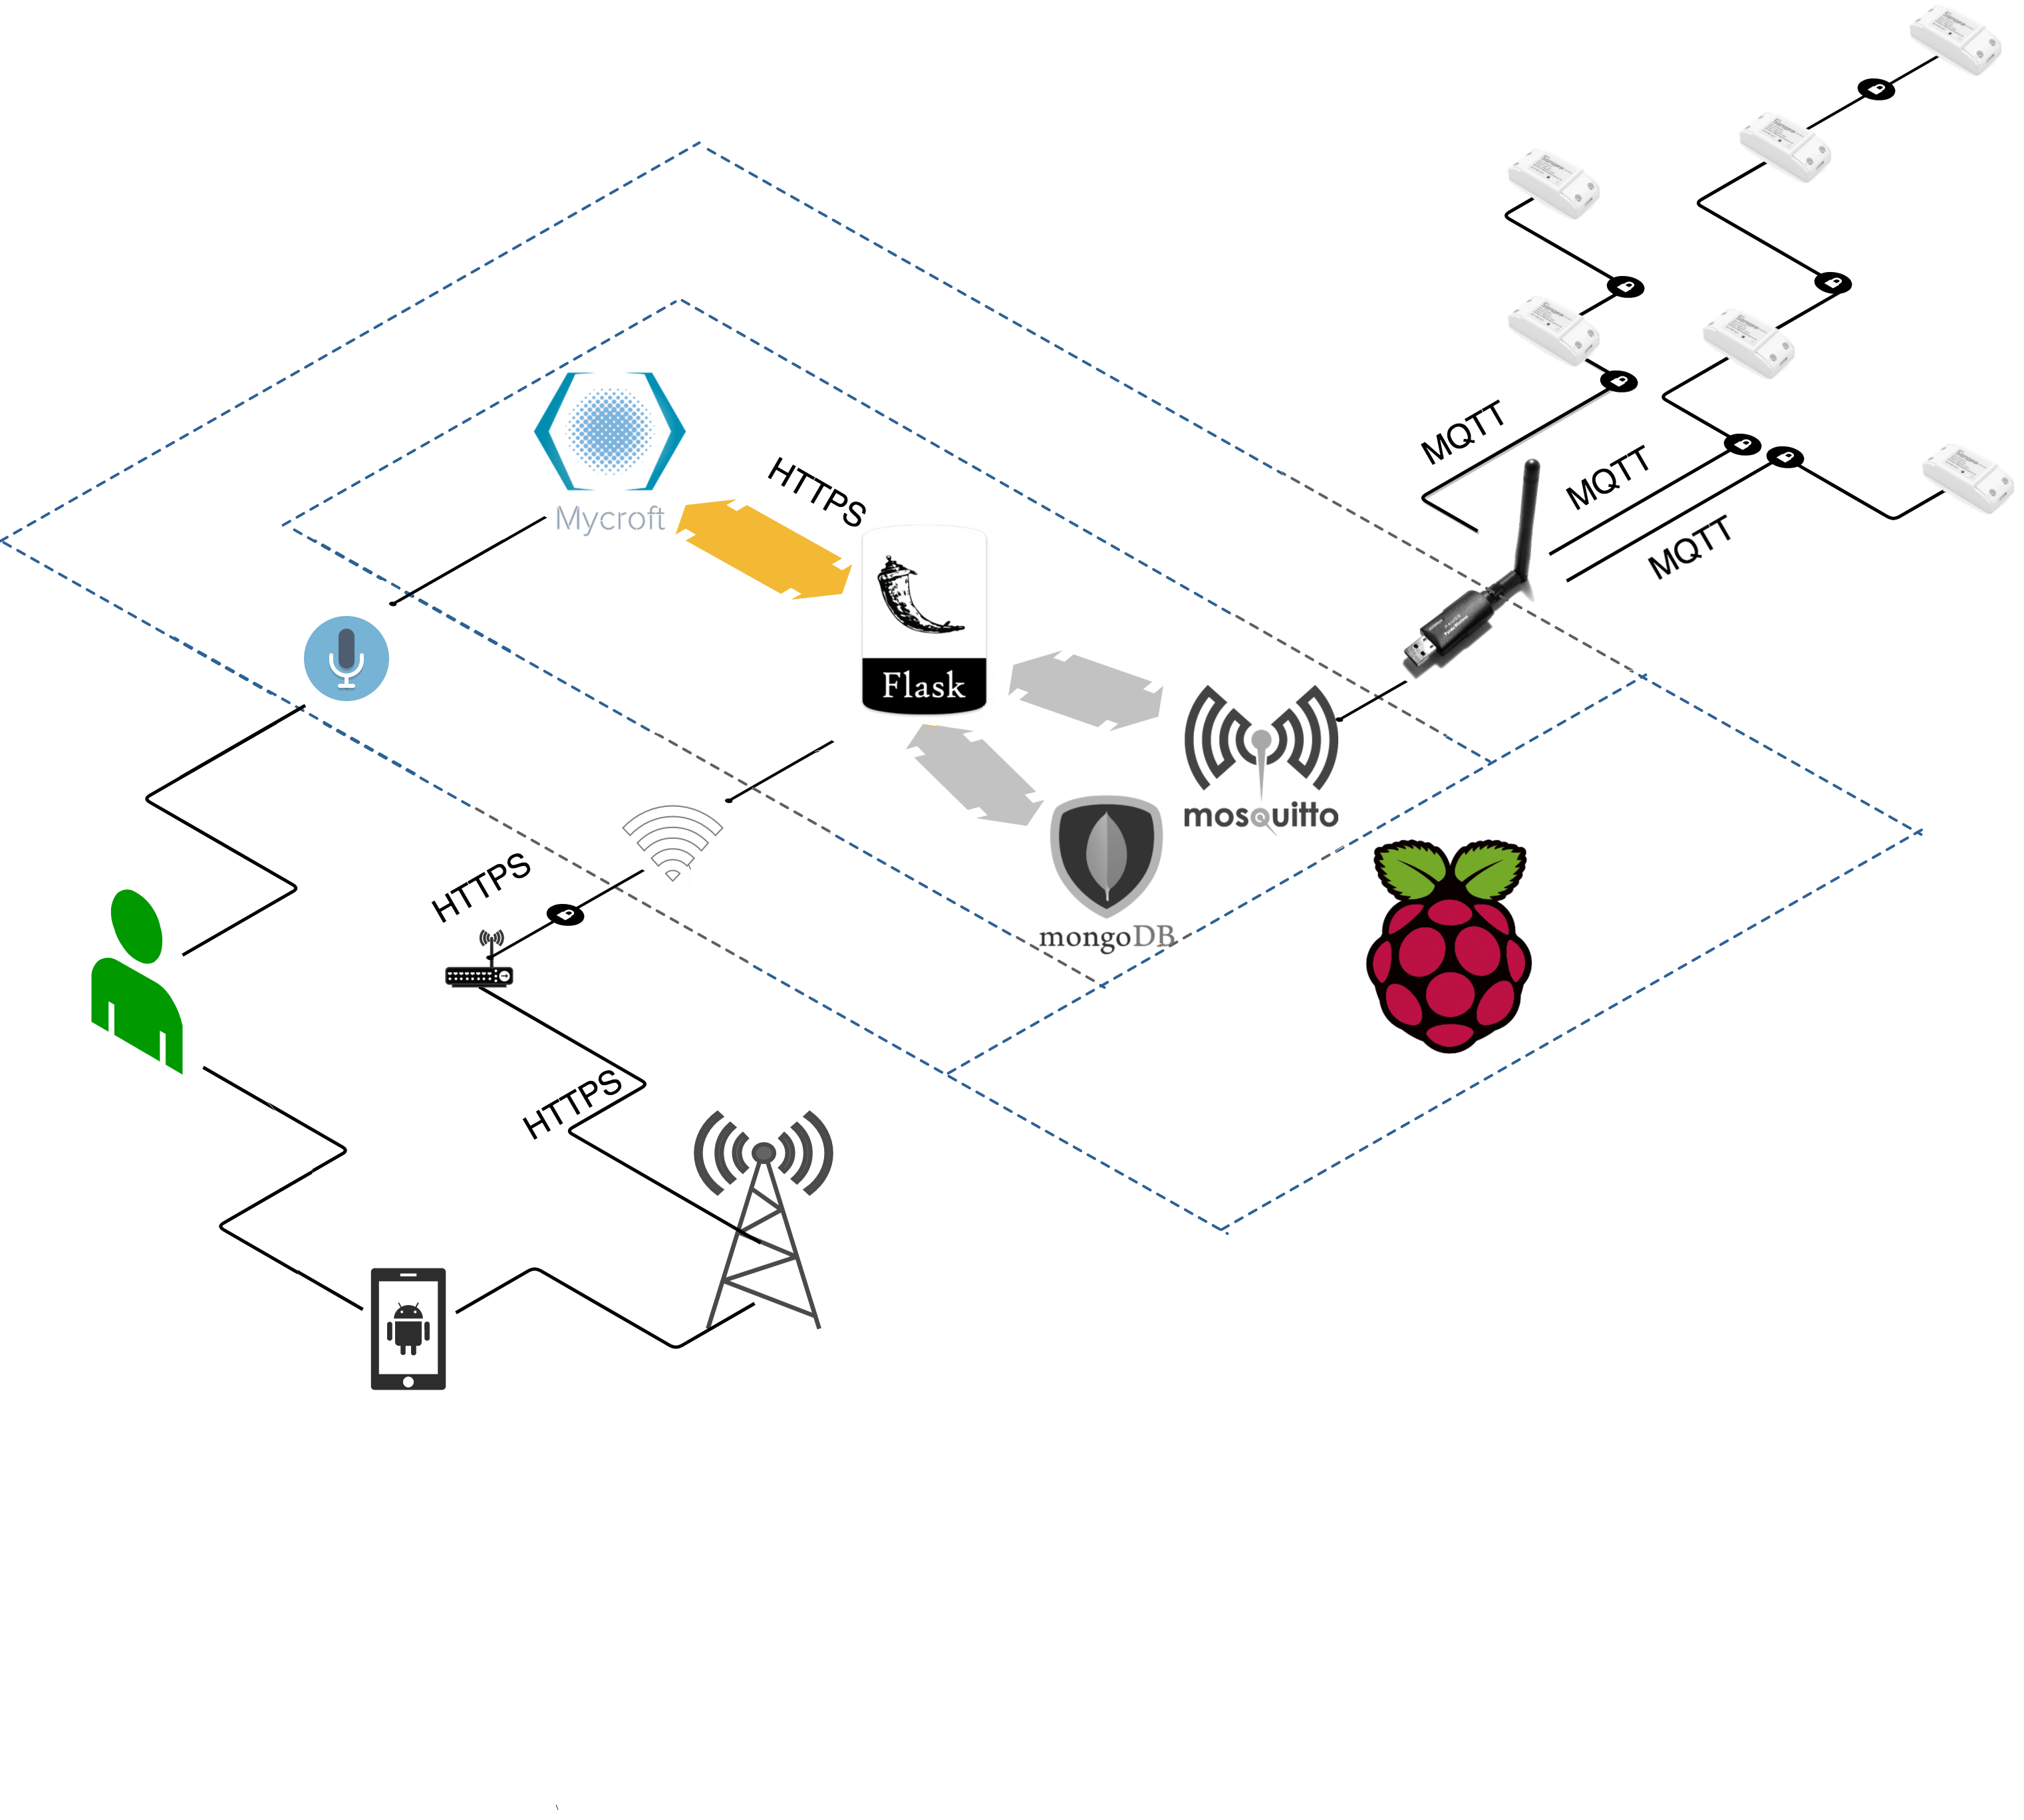
\includegraphics[width=0.6\textwidth, keepaspectratio]{images/mod-ui-mycroft}
  \caption{\textit{Componentes del Módulo de UI para Asistente Virtual.}}
  \label{fig:mod-ui-mycroft}
\end{figure}

\paragraph{Descripción:}

\begin{itemize}
\item Utilizando Mycroft, se permite el control a través de voz a los dispositivos ya configurados en el sistema.
\end{itemize}


\section{Desarrollo}

\subsection{Módulo MQTT Mesh}

Este módulo cuenta con el broker mosquitto localizado en el Raspberry Pi y el firmware desarrollado para este proyecto en los dispositivos Sonoff.

\subsubsection{Mosquitto broker:} \label{mosquitto-broker}
Primero se debe acceder al Raspberry Pi a través de ssh e instalar los componentes:

\begin{lstlisting}[language=bash]
  $ sudo apt-get update
  $ sudo apt-get upgrade
  $ sudo apt-get install mosquitto
  $ sudo apt-get install mosquitto-clients
\end{lstlisting}

Luego se debe realizar un link simbólico del archivo de configuración proveído en el repositorio de GitHub del proyecto, dentro de \lstinline[columns=fixed]{MQTT_Server/mosquitto}. Para lograr esto, se debe posicionar en la carpeta del Raspberry Pi que contiene el archivo de configuración creado en la instalación de mosquitto, la dirección predeterminada es \lstinline[columns=fixed]{/etc/mosquitto}, luego se debe borrar este archivo y crear un link con el archivo anteriormente mencionado.

\begin{lstlisting}[language=bash]
  $ sudo rm mosquitto.conf
  $ sudo ln -s <cloned repo directory>/Tesis/MQTT_Server/mosquitto/mosquitto.conf mosquitto.conf
\end{lstlisting}

El contenido del archivo al cual se crea el link es el siguiente:
\begin{lstlisting}[language=bash]
pid_file /var/run/mosquitto.pid

persistence true
persistence_location /var/lib/mosquitto/

log_dest file /var/log/mosquitto/mosquitto.log
allow_anonymous false
password_file /etc/mosquitto/pwfile
listener 1883
\end{lstlisting}

Algunos puntos importantes de esta configuración son:


\paragraph{persistence}: 
Si es seteado a \lstinline[columns=fixed]{True}, toda conexión suscripción y mensajes serán escritos en el disco, en una base de datos llamada \lstinline[columns=fixed]{mosquitto.db}, localizada en la carpeta indicada por \lstinline[columns=fixed]{persistence_location}. Cuando mosquitto se reinicia, carga toda la información contenida en esta base de datos. Los datos se guardan en la base de datos cuando mosquitto se cierra o en intervalos de tiempo definidos por \lstinline[columns=fixed]{autosave_interval}. Se puede forzar un guardado en la base de datos enviando a mosquitto la señal \lstinline[columns=fixed]{SIGUSR1}.

\paragraph{allow\_anonymous}:
También de valor booleano, determina si los clientes deben proveer o no nombre de usuario y contraseña al conectarse. Si se setea a false, se debe crear otro medio de autenticación para el acceso de clientes. Su valor predeterminado es true.

Al indicar que sólo aceptaremos conexiones que brinden credenciales, debemos crear la contraparte verificadora de las mismas en el broker, para esto, se debe correr el siguiente comando:

\begin{lstlisting}[language=bash]
  $ sudo mosquitto_passwd -c /etc/mosquitto/pwfile <username>
\end{lstlisting}

Para testear que esto haya funcionado correctamente se puede inicializar un cliente con las credenciales configuradas en el archivo recién creado de la siguiente forma: 

\begin{lstlisting}[language=bash]
  $ mosquitto_sub -d -u <username> -P <passwd> -t test/topic
\end{lstlisting}

Y se debería obtener el siguiente resultado:

\begin{lstlisting}[language=bash]
  $ Client mosqsub/8161-picroft sending CONNECT
  $ Client mosqsub/8161-picroft received CONNACK
  $ Client mosqsub/8161-picroft sending SUBSCRIBE (Mid: 1, Topic: /test/topic, QoS: 0)
  $ Client mosqsub/8161-picroft received SUBACK
  $ Subscribed (mid: 1): 0
\end{lstlisting}

Luego utilizando la misma herramienta publicar un mensaje en el topic al que nos suscribimos (utilizaremos las mismas credenciales ya que son las únicas que se configuran, aunque esto no es necesario) :

\begin{lstlisting}[language=bash]
  $ mosquitto_pub -d -u <username> -P <passwd> -t test/channel -m whatever
\end{lstlisting}

En la consola del cliente suscrito se debería obtener:

\begin{lstlisting}[language=bash]
  $ pi@picroft:~ $ mosquitto_pub -d -t /test/channel -m whatever
Client mosqpub/8164-picroft sending CONNECT
Client mosqpub/8164-picroft received CONNACK
Client mosqpub/8164-picroft sending PUBLISH (d0, q0, r0, m1, '/test/channel', ... (8 bytes))
Client mosqpub/8164-picroft sending DISCONNECT

  $ pi@picroft:/etc/mosquitto $ mosquitto_sub -d -t /test/channel

Client mosqsub/8163-picroft sending CONNECT
Client mosqsub/8163-picroft received CONNACK
Client mosqsub/8163-picroft sending SUBSCRIBE (Mid: 1, Topic: /test/channel, QoS: 0)
Client mosqsub/8163-picroft received SUBACK
Subscribed (mid: 1): 0
Client mosqsub/8163-picroft received PUBLISH (d0, q0, r0, m0, '/test/channel', ... (8 bytes))
whatever
\end{lstlisting}

\subsubsection{Access Point:}

Se conectó un dongle de wifi al Raspberry Pi para poder crear una red dedicada a la comunicación entre los elementos de la red, ya que se quería independizar la misma de la red wifi del lugar de instalación.~\cite{AccessPoint}

\begin{itemize}

\item Primero instalar componentes:

\begin{lstlisting}[language=bash]
sudo apt-get update
sudo apt-get install hostapd isc-dhcp-server
sudo apt-get install iptables-persistent
\end{lstlisting}

Aparecerán dos ventanas de configuración, elegir "Yes" en las dos.
\item Configurar el DHCP server
Editaremos el archivo \lstinline[columns=fixed]{/etc/dhcp/dhcpd.conf}.

\begin{lstlisting}[language=bash]
sudo nano /etc/dhcp/dhcpd.conf
\end{lstlisting}

Encontrar las siguientes líneas y comentarlas:

\begin{lstlisting}[language=bash]
option domain-name "example.org";
option domain-name-servers ns1.example.org, ns2.example.org;
\end{lstlisting}

Encontrar las siguientes líneas y descomentar "authoritative":

\begin{lstlisting}[language=bash]
# If this DHCP server is the official DHCP server for the local
# network, the authoritative directive should be uncommented.
# authoritative
\end{lstlisting}

Por último se recorre hasta el final del archivo y se agrega:

\begin{lstlisting}[language=bash]
subnet 192.168.42.0 netmask 255.255.255.0 { 
  range 192.168.42.10 192.168.42.50;
  option broadcast-address 192.168.42.255;
  option routers 192.168.42.1;
  default-lease-time 600;
  max-lease-time 7200;
  option domain-name "local";
  option domain-name-servers 8.8.8.8, 8.8.4.4;
}
\end{lstlisting}

Ejecutar:
\begin{lstlisting}[language=bash]
sudo nano /etc/default/isc-dhcp-server
Y buscar INTERFACES="", agregar el nombre de la interfaz del adaptador de WiFi.
\end{lstlisting}

\item Luego se fija una IP estática para esta interfaz, para esto debemos modificar el archivo \lstinline[columns=fixed]{/etc/network/interfaces}:

\begin{lstlisting}[language=bash]
sudo nano /etc/network/interfaces
\end{lstlisting}

Se agrega las siguientes líneas luego de allow-hotplug wlan0:

\begin{lstlisting}[language=bash]
iface wlan0 inet static
address 192.168.42.1
netmask 255.255.255.0
\end{lstlisting}

\item Configurar Access Point. \\
Se crea un nuevo archivo \lstinline[columns=fixed]{/etc/hostapd/hostapd.conf} con la configuración:

\begin{lstlisting}[language=bash]
interface=wlan0
driver=nl80211
ssid=Pi_AP
country_code=US
hw_mode=g
channel=6
macaddr_acl=0
auth_algs=1
ignore_broadcast_ssid=0
wpa=2
wpa_passphrase=Raspberry
wpa_key_mgmt=WPA-PSK
wpa_pairwise=CCMP
wpa_group_rekey=86400
ieee80211n=1
wme_enabled=1
\end{lstlisting}

Por último se debe indicar al RPi dónde encontrar el archivo de configuración:

\begin{lstlisting}[language=bash]
sudo nano /etc/default/hostapd
\end{lstlisting}

En la línea que dice \lstinline[columns=fixed]{#DAEMON_CONF=""} sustituir por:

\begin{lstlisting}[language=bash]
DAEMON_CONF="/etc/hostapd/hostapd.conf"
\end{lstlisting}
\end{itemize}

\subsubsection{Dispositivos Sonoff}

\paragraph{Modificaciones físicas y subida de firmware}
 A pesar de que este componente está pensado para ser hackeado, es necesario realizarle algunas modificaciones físicas poder modificar el firmware del mismo.

\begin{figure}[h]
  \centering
  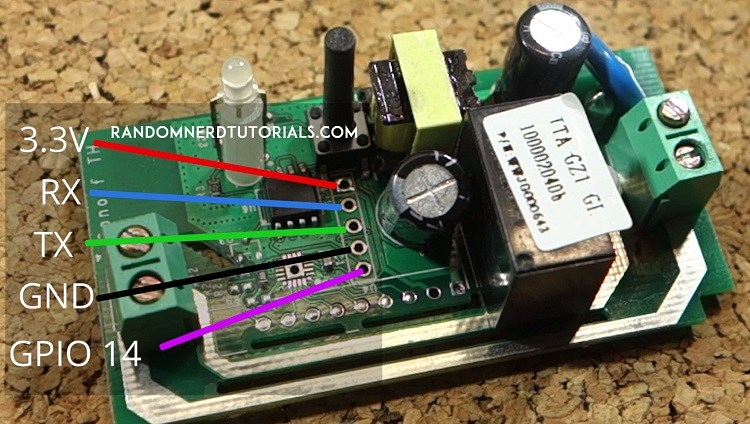
\includegraphics[width=0.6\textwidth, keepaspectratio]{images/sonoff-gpio}
  \caption{\textit{Conexiones del ESP8266 expuestas por el Sonoff.}}
  \label{fig:sonoff-gpio}
\end{figure}
En la figura~\qref{fig:sonoff-gpio} podemos apreciar que los conectores del chip ESP8266 integrado en el Sonoff son fácilmente accesibles pero no cuentan con cabezales para conectar los cables del adaptador Serial-USB, por esta razón es necesario soldar los mismos.
Luego se debe conectar al adaptador USB/Serial ~\qref{fig:images/sonoff-modified} para poder subir el firmware desde un computador. 

\begin{figure}[h!]
  \centering

  \begin{subfigure}[b]{0.5\textwidth}
    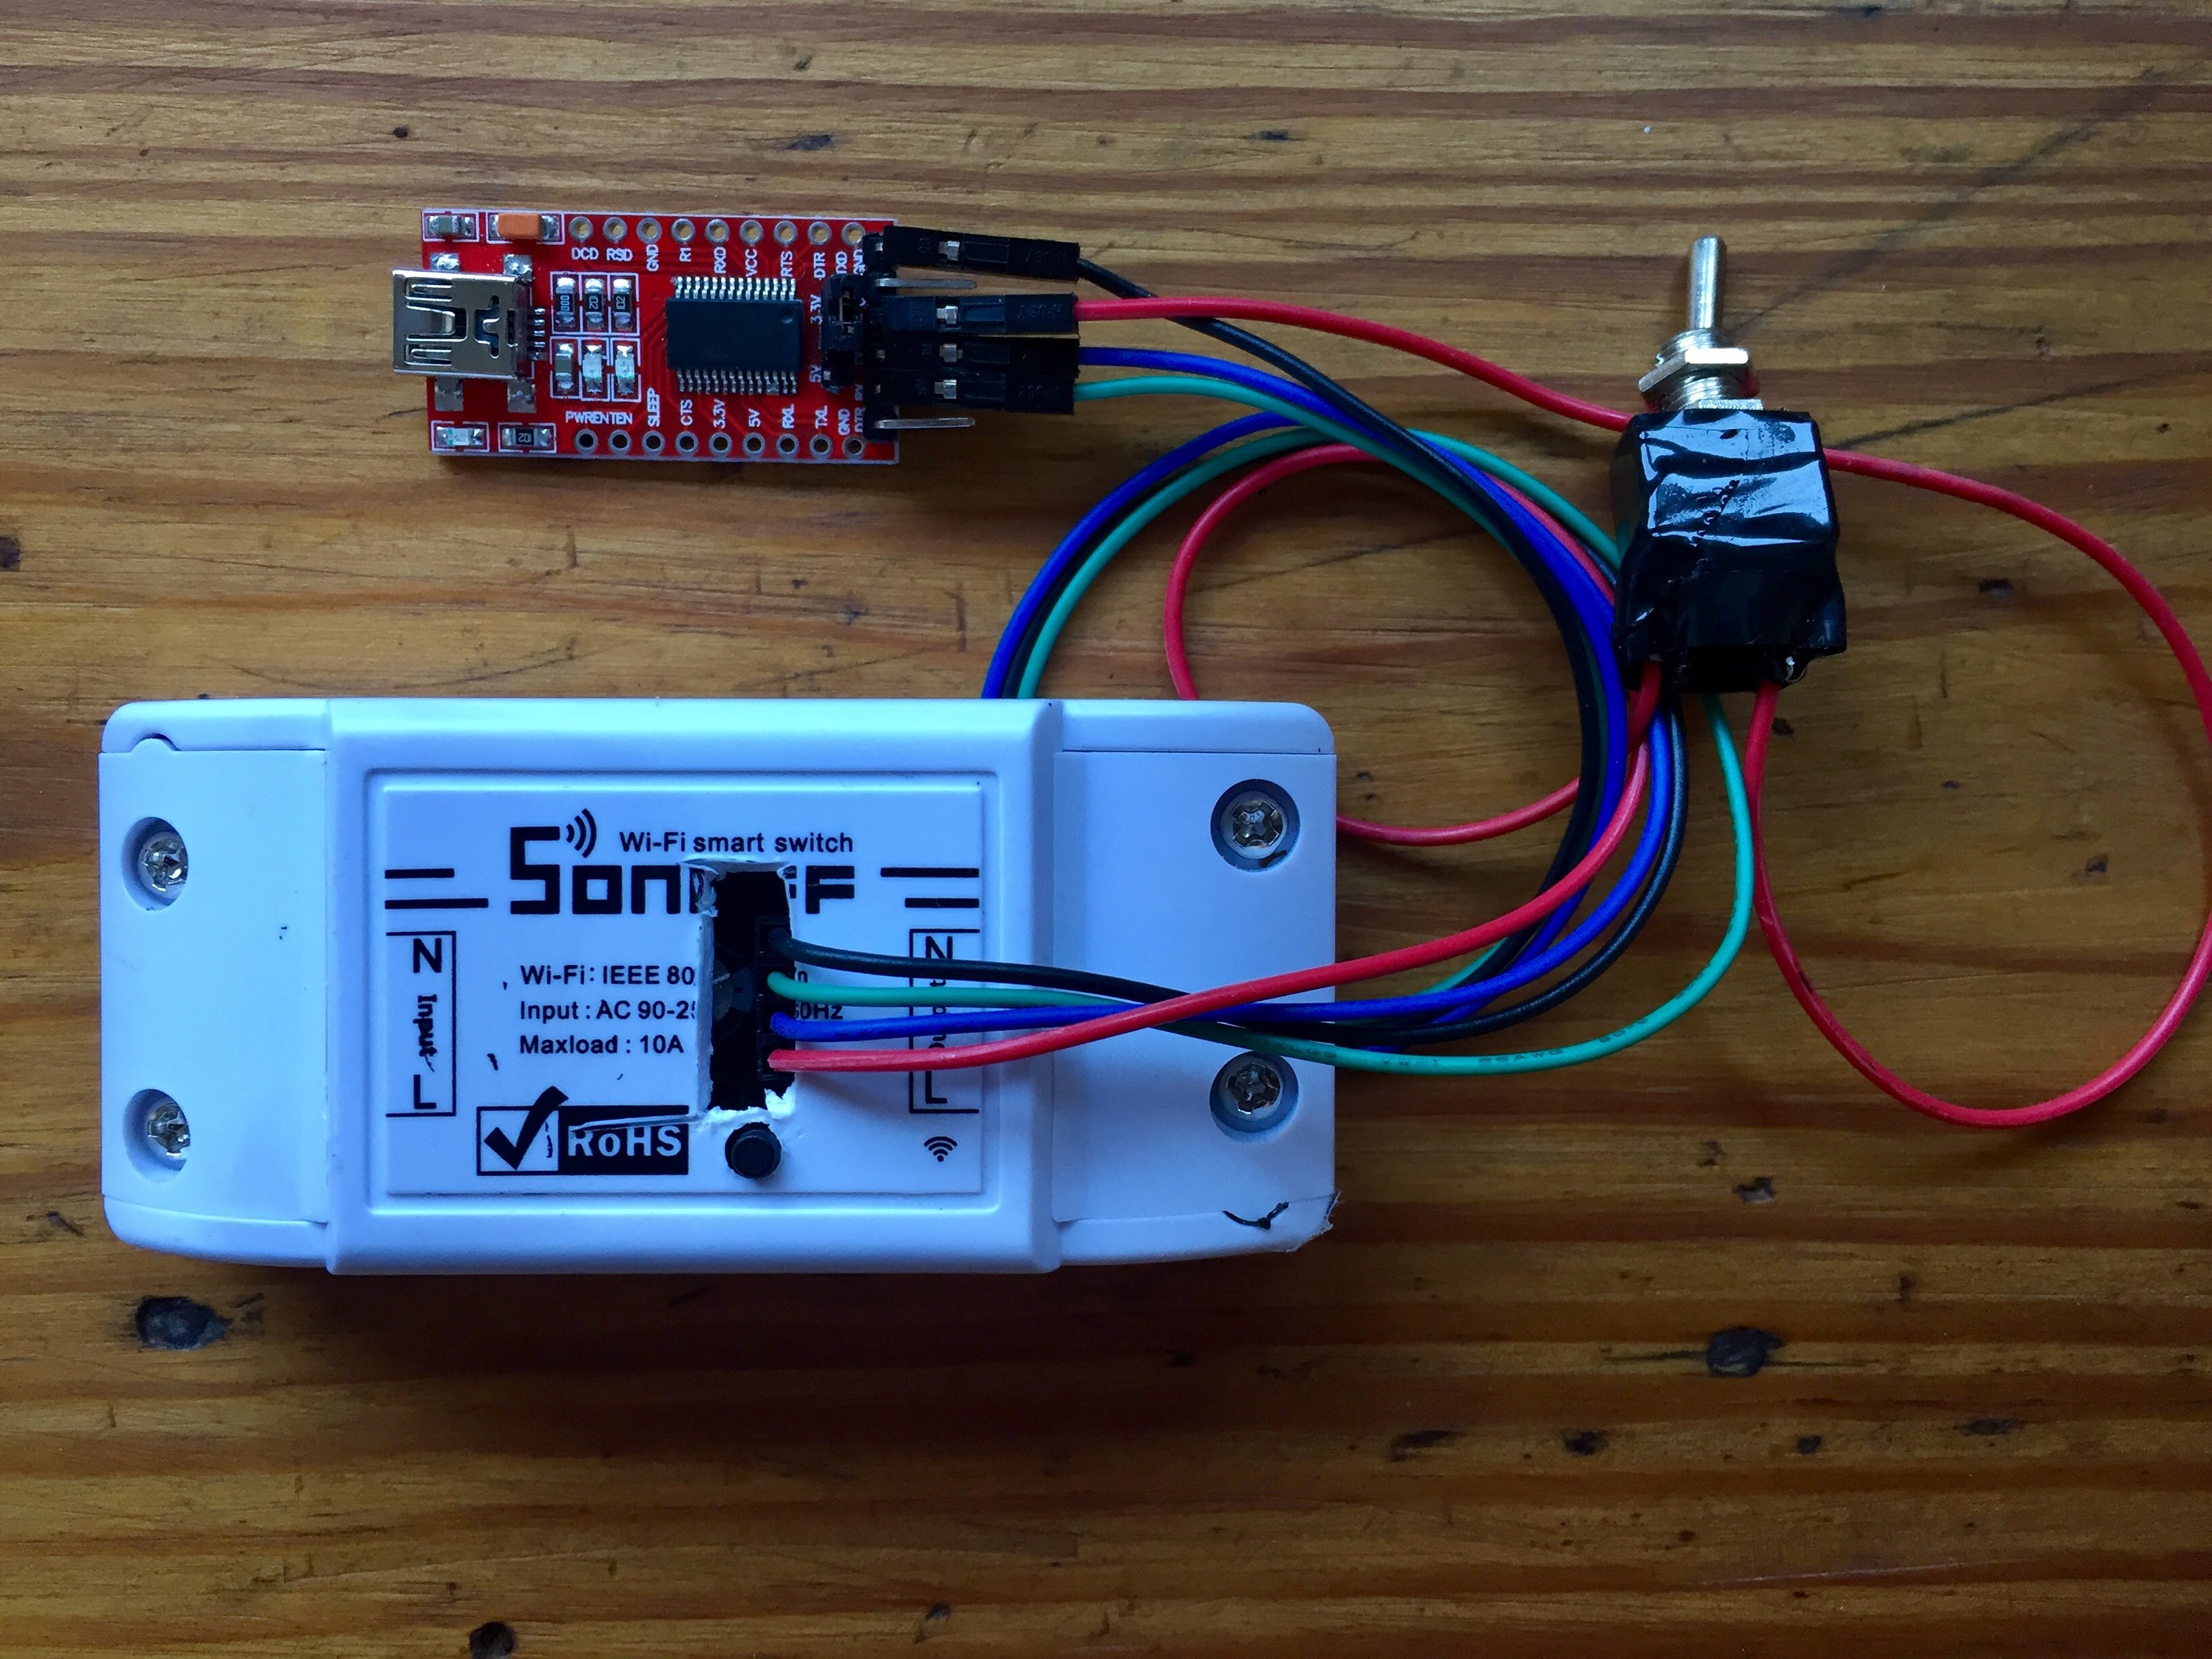
\includegraphics[width=\textwidth, keepaspectratio]{images/sonoff-modified}
    \caption{\textit{Vista superior..}}
    \label{fig:images/sonoff-modified}
  \end{subfigure}
  %
  \begin{subfigure}[b]{0.5\textwidth}
    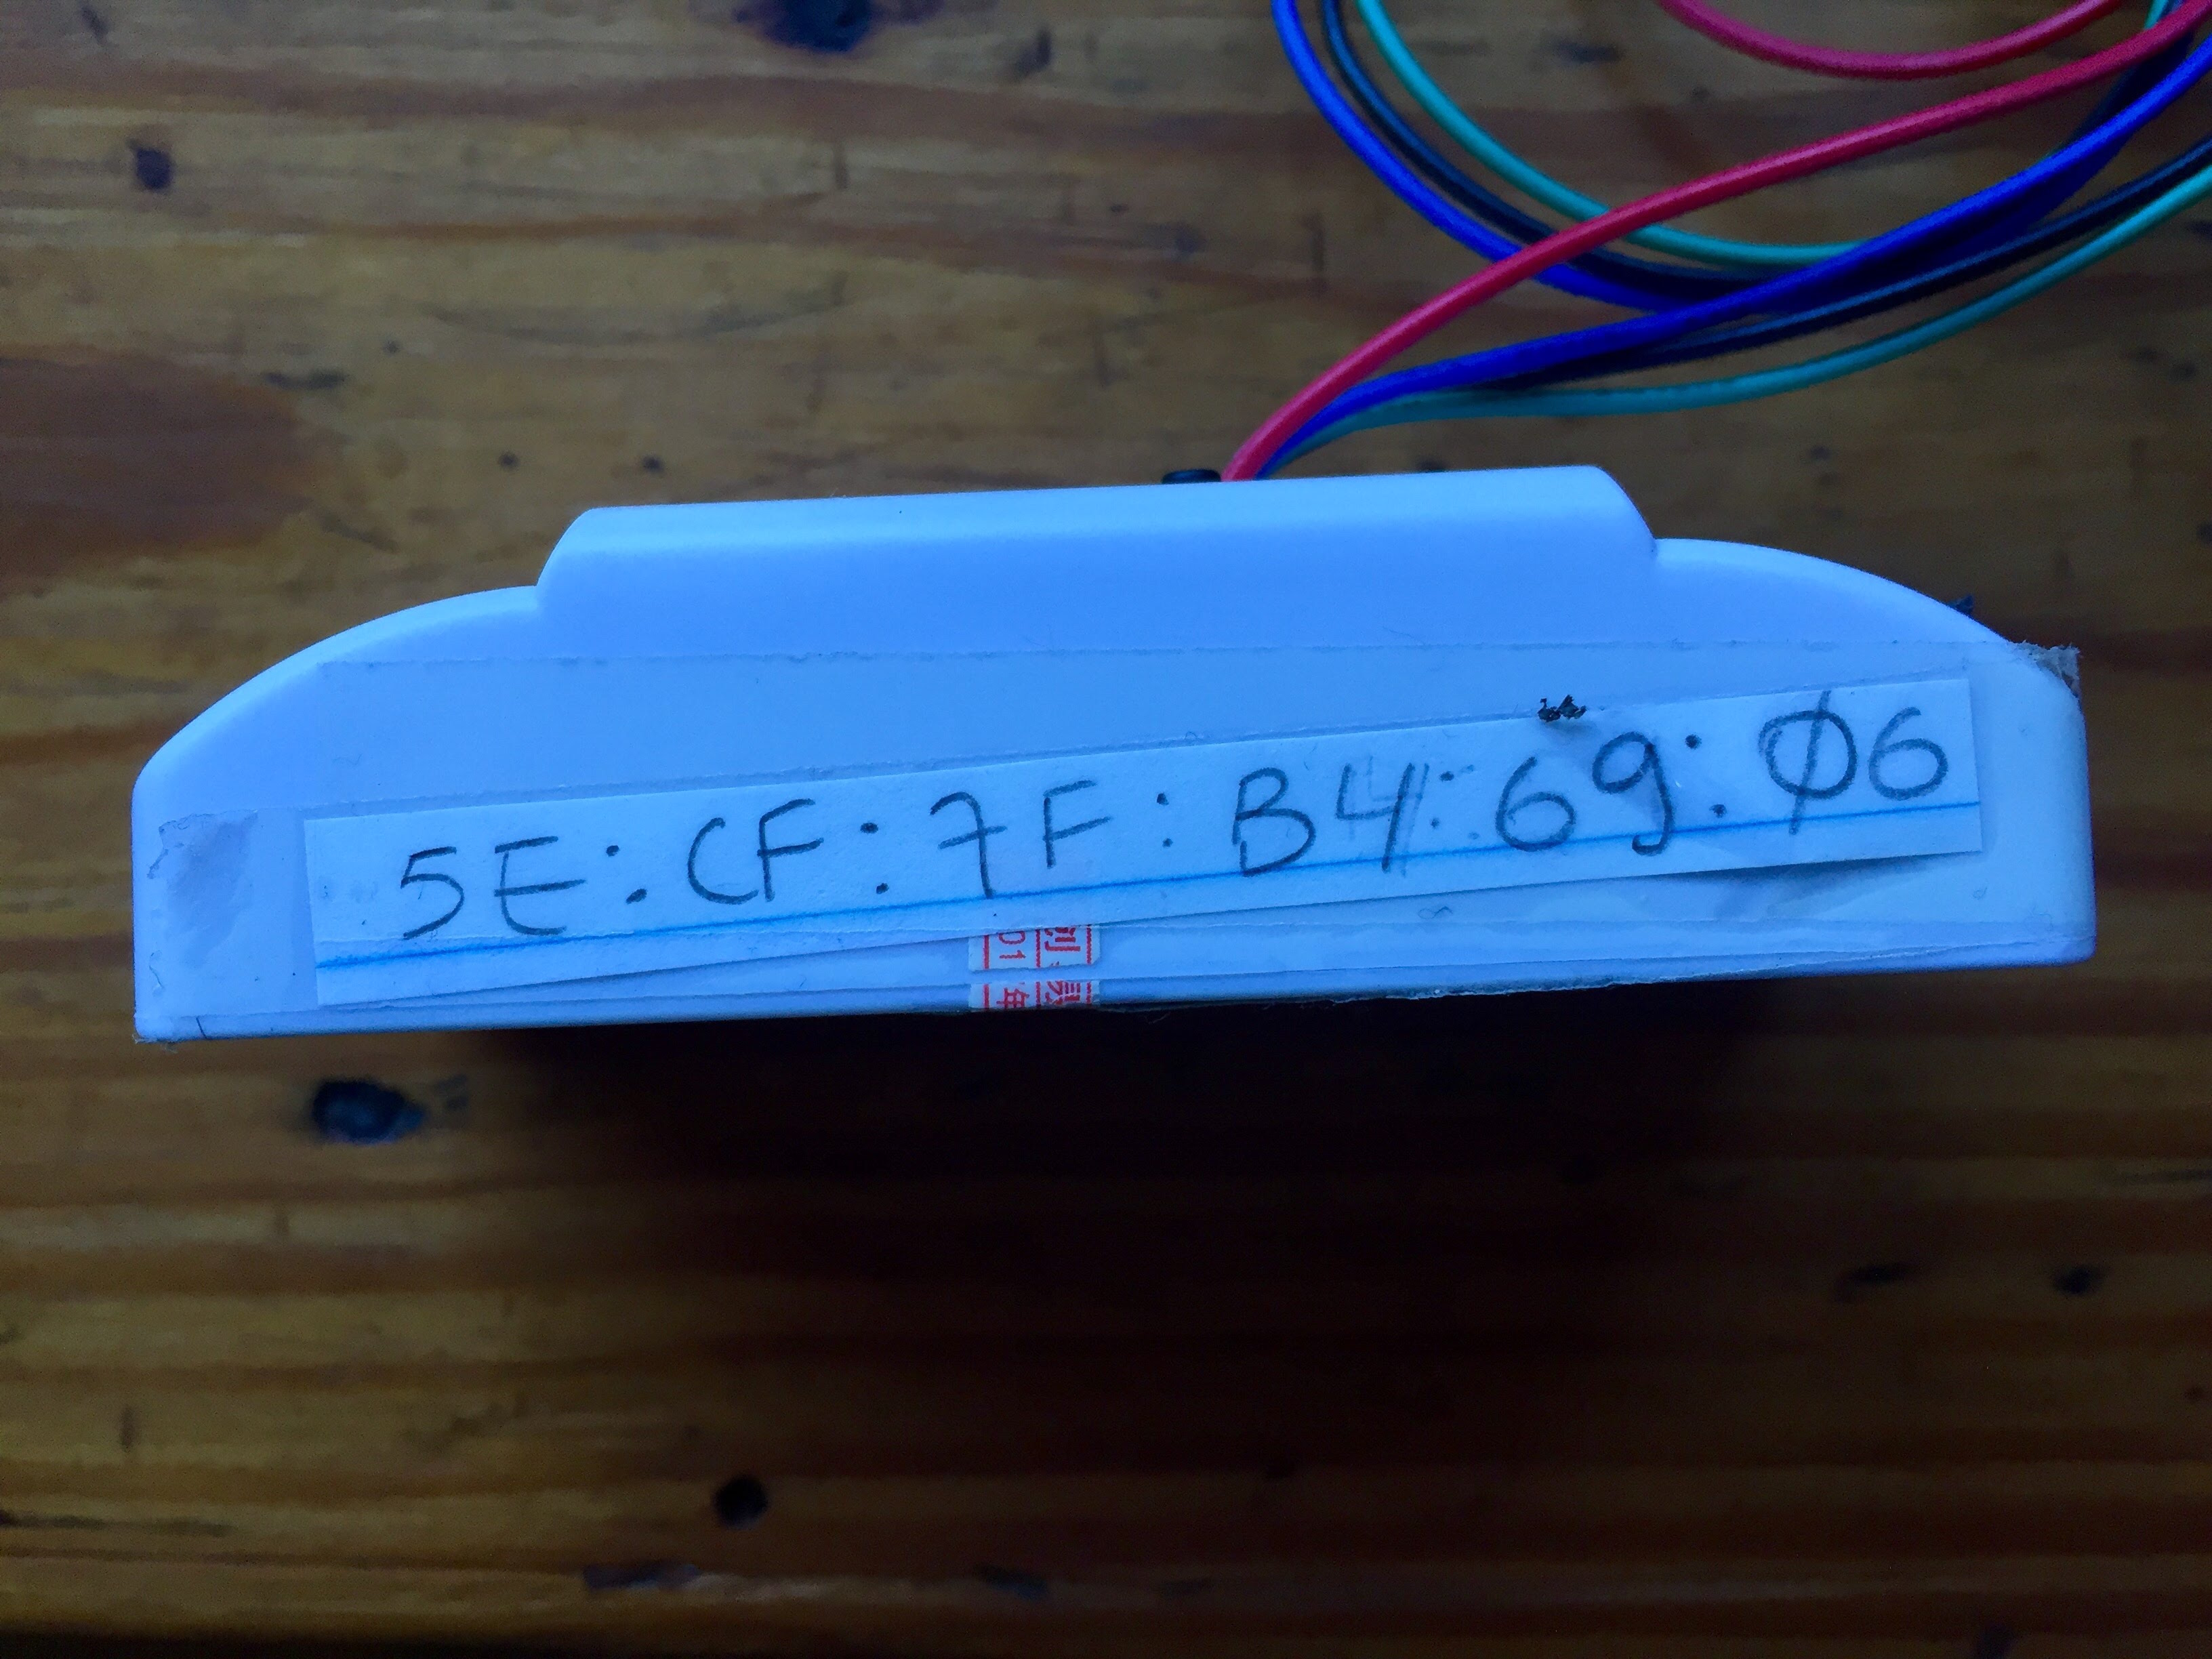
\includegraphics[width=\textwidth, keepaspectratio]{images/sonoff-side}
    \caption{\textit{Vista de lado.}}
    \label{fig:sonoff-side}
  \end{subfigure}

\caption{\textit{Sonoff modificado.}}
\end{figure}

\subparagraph{Adaptación de interruptores analógicos}\mbox{}\\

Debido a que se busca la mayor comodidad del lado del usuario y se intenta que la integración del sistema no conlleve a limitaciones, se configuraron los dispositivos Sonoff para poder ser controlados por interruptores analógicos. Ya sea del tipo utilizado comunmente en instalaciones eléctricas como interruptores digitales.
Esto permitirá que el usuario utilizar tanto los medios usuales como las interfaces desarrolladas para interactuar con el sistema. Esto se logra conectando el interruptor entre el \lstinline[columns=fixed]{pin GPIO14}~\qref{fig:sonoff-interruptor} del Sonoff y tierra. logrando asi una interacción lógica con el relay interno.

\begin{figure}[h]
  \centering
  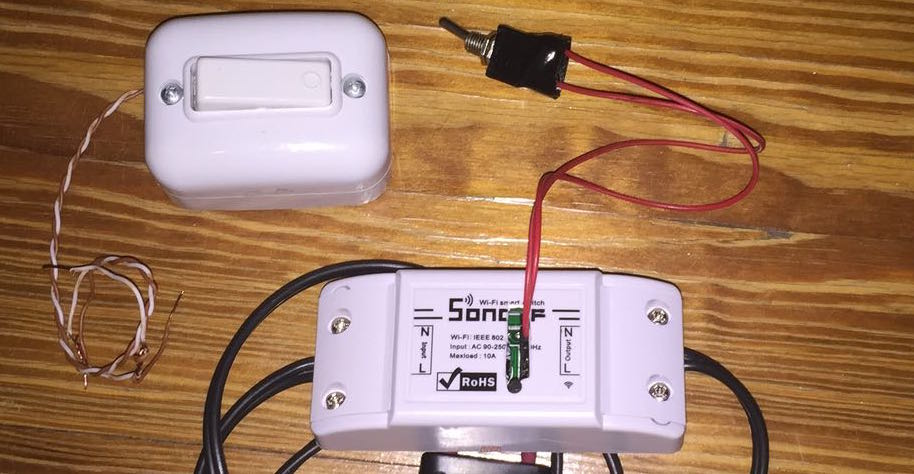
\includegraphics[width=0.6\textwidth, keepaspectratio]{images/sonoff-switch}
  \caption{\textit{Conexion de interruptores con Sonoff.}}
  \label{fig:sonoff-interruptor}
\end{figure}

Esto permite que si el usuario apaga las luces con llave en la pared, luego las enciende con la aplicación y a continuación oprime la llave en la pared, la luz volverán a apagarse.
Este comportamiento permite una interacción más natural e intuitiva, siendo la falta de esta funcionalidad una debilidad clave en las soluciones de la competencia.

Para lograr que el interruptor tenga comportamiento de botón que cambie de estado el relay, se debío configurar el pin en modo \lstinline[columns=fixed]{INPUT_PULLUP}, para luego vincular este pin con una interrupción que dispare la función \lstinline[columns=fixed]{switch_state_changed}.
Esta función cambia de estado al relay y envía una notificación al servidor central para informar el estado del dispositivo. Este mensaje se envía en el topic \lstinline[columns=fixed]{device_out/sub_topic/state_changed} siendo la estructura del mensaje enviado:

\begin{lstlisting}
 {
  "_id": {_id},
  "state": "0/1"
 }
\end{lstlisting}

La configuración y vinculación de la interrupción se logran con las siguientes líneas:

\begin{lstlisting}[language=C]
  //Setup the Switch :
  pinMode(SWITCH_PIN, INPUT_PULLUP);
  attachInterrupt(digitalPinToInterrupt(SWITCH_PIN), switch_state_changed, CHANGE);
\end{lstlisting}

Como se puede observar la función se ejecuta con la condición \lstinline[columns=fixed]{CHANGE}, por lo que no diferencia entre interruptor cerrado o abierto.
Observando la función llamada, podemos notar algunas singularidades, por ejemplo, es necesario utilizar una lógica de semáforo por temporizador, ya que debido a la imperfección de los interruptores analógicos, el chip detecta diferentes cantidades de cambios en el interruptor antes de cambiar de estado, esto es conocido como efecto rebote.

\begin{lstlisting}[language=C]
void switch_state_changed () {
  unsigned long interrupt_time = millis();
  if (interrupt_time - previousInterrupt > 200)
  {
    previousInterrupt = interrupt_time;
    int state = digitalRead(RELAY_PIN);
    digitalWrite(RELAY_PIN, !state);
    char msg[255];
    strlcpy(msg, "{", sizeof(msg));
    strlcat(msg, "\"_id\":", sizeof(msg));
    strlcat(msg, ID.c_str(), sizeof(msg));
    strlcat(msg, ",\"state\":", sizeof(msg));
    if(state==0)strlcat(msg, "\"0\"", sizeof(msg));
    if(state==1)strlcat(msg, "\"1\"", sizeof(msg));
    strlcat(msg, "}", sizeof(msg));
    mesh->publish(
      "state_changed",
      msg
    );
  }
}
\end{lstlisting}


Cabe mencionar que este efecto no es provocado solamente por cambios de estado del interruptor externo conectado al Sonoff, sino que al realizar pruebas y modificar el estado del relay desde la aplicación móvil, se descubrió que al prenderse el relay, los cambios de tensión disparaban la interrupción. Por lo que se debió activar el semáforo en caso de recibir órdenes remotas, para evitar que esta situación entorpezca el funcionamiento del dispositivo.

\begin{lstlisting}[language=C]
if(sTopic == "Power"){//Relay HIGH to turn on
    previousInterrupt = millis();
    ...
}
\end{lstlisting}


\paragraph{Análisis de Código}

\subparagraph{Librería FS}~\qref{sec-SPIFFS}\mbox{}\\

Esta librería es usada por la librería \lstinline[columns=fixed]{ESP8266MQTTMesh}~\qref{anexo-esp8266mqttmesh} y también en el código que se realizó. Para lo primero que se utilizó como se puede ver a continuación,  es para leer de los \lstinline[columns=fixed]{SPIFFS} y así ver si existe una variable llamada \lstinline[columns=fixed]{mqtt_server} donde se almacena la IP del broker MQTT. Si no encuentra este archivo se conecta a  la red MQTT con la IP por default que tiene el broker en el archivo \lstinline[columns=fixed]{credentials.h}.

\begin{lstlisting}[language=C]
broker=getInformationFromSPIFFS("/broker/");
 if(broker!=""){//getInformationFromSPIFFS("/broker/")
    mqtt_server=broker.c_str();
  }else{
    mqtt_server=mqtt_default_server;
  }

String getInformationFromSPIFFS(String baseString){
  Dir dir = SPIFFS.openDir(baseString);
  if(!dir.next()){
    return "";
  }else{
    File brokerFile=SPIFFS.open(dir.fileName(), "w");
    char* str=(char*)brokerFile.name();
    char * pch;
    pch = strtok (str,"/");
    int counter=0;
    String broker;
    while (pch != NULL)  {
        if(counter==1){
          broker=String(pch);
        }
        Serial.println("entre");
        pch = strtok (NULL, "/");
        counter=counter+1;
    }
    return broker;
  }
}
\end{lstlisting}

Si se quisiera, también se podría usar el mismo concepto con otras variables que se encuentran en el archivo \lstinline[columns=fixed]{credentials.h} como \lstinline[columns=fixed]{MESH_PASSWORD}, \lstinline[columns=fixed]{MQTT_DEFAULT_SERVER}, \lstinline[columns=fixed]{NETWORK_LIST}. Esto hace que los valores del archivo \lstinline[columns=fixed]{credentials.h} sean flexibles. 

Esta librería también se utiliza para variables que no están en \lstinline[columns=fixed]{credentials.h}. Por ejemplo, para determinar si dejar pasar la electricidad en el relé al momento de prender el Sonoff. Este se fija si existe la el directorio \lstinline[columns=fixed]{/ON_When_Power_On/}, si existe, deja pasar la electricidad. De la misma manera se fija si existe el directorio \lstinline[columns=fixed]{/OFF_When_Power_On/} para determinar no deja pasar la electricidad. Se utiliza el método \lstinline[columns=fixed]{SPIFFS.exists(path)} de forma trivial. Ya se explicó anteriormente su funcionamiento básico.[~\qref{sec-SPIFFS}]

\begin{lstlisting}[language=C]
boolean bONExists = check_if_power_ON_Exists();
boolean bOFFExists = check_if_power_OFF_Exists();

  //check if poweroff or on state exists in spiffs
  if (!bONExists && !bOFFExists) {
    File f = SPIFFS.open("/ON_When_Power_On/", "w");//por defecto esta ON
    f.close();
    digitalWrite(RELAY_PIN, HIGH);
  } else {
    if (bONExists){
      digitalWrite(RELAY_PIN, HIGH);
    }else{
      if (bOFFExists){
        digitalWrite(RELAY_PIN, LOW);
      }
    }
  }
\end{lstlisting}

\subparagraph{Librería Bounce2}}\mbox{}\\
Esta es una librería de Arduino que sirve para cubrirse de los problemas típicos de rebotes asociados a la utilización de botones en el hardware. Se setea el pin asociado al botón como una entrada pull up de la siguiente manera:


\begin{lstlisting}[language=C]
pinMode(BUTTON_PIN,INPUT_PULLUP);
\end{lstlisting}

Luego se crea el objeto asociado a esta librería:

\begin{lstlisting}[language=C]
Bounce debouncer = Bounce();
\end{lstlisting}

Se crea un vínculo entre el objeto y el pin asociado al botón y se setea el tiempo de rebote en milisegundos:

\begin{lstlisting}[language=C]
debouncer.attach(BUTTON_PIN);
debouncer.interval(5); // interval in ms
\end{lstlisting}

Dentro del loop se actualiza el objetivo para que tome el valor del pin donde está el botón y  se lee ese valor:

\begin{lstlisting}[language=C]
debouncer.update();
int value = debouncer.read();
\end{lstlisting}

Esto se usa para ver si el usuario aprieta el botón más de 2 segundos, si esto pasa es porque se quiere entrar en el modo de configuración del Sonoff.

\subparagraph{Librería ESP8266MQTTMesh}\mbox{}\\

Esta librería es la base del proyecto. La misma se encarga de setear una \lstinline[columns=fixed]{IP} única para cada nodo de la red. Hace esto basándose en una propiedad que tiene el broker mosquitto que consiste en que cada vez que un dispositivo se suscribe a él. Este publica la bssid de todos los nodos que se han conectado. La bssid se crea en base a la \lstinline[columns=fixed]{MAC} del dispositivo que se suscribió con un número identificador de la siguiente forma: 

\begin{lstlisting}[language=bash]
Client mosqsub/2372-picroft received PUBLISH (d0, q0, r1, m0, '/device_in/bssid/2E:3A:E8:11:60:A3', ... (1 bytes))
4
Client mosqsub/2372-picroft received PUBLISH (d0, q0, r1, m0, '/device_in/bssid/5E:CF:7F:B4:69:06', ... (1 bytes))
5
Client mosqsub/2372-picroft received PUBLISH (d0, q0, r1, m0, '/device_in/bssid/2E:3A:E8:0F:43:95', ... (1 bytes))
7
\end{lstlisting}

Es así que el nodo toma esas \lstinline[columns=fixed]{BSSID} y ve si la suya coincide con alguna de las publicadas. Si es así, se setea la \lstinline[columns=fixed]{IP} \lstinline[columns=fixed]{192.168.<subdominio>.1} siendo subdominio el número único expuesto anteriormente. Si no coincide con ninguna, hace una iteración desde 4 hasta 256 hasta que encuentra un número no coincida con ninguno de los números únicos y se setea ese como subdominio. Esta \lstinline[columns=fixed]{IP} es almacenada en las \lstinline[columns=fixed]{SPIFFS} por si la próxima vez que se inicie no llega al broker para conseguir su \lstinline[columns=fixed]{IP}, toma la que tiene guardada en \lstinline[columns=fixed]{SPIFFS}.

En el nodo, la red mesh se inicializa de la siguiente manera:

\begin{lstlisting}[language=bash]
mesh = ESP8266MQTTMesh::Builder(networks, network_password, (char*)mqtt_server, mqtt_port)
  .setVersion(FIRMWARE_VER, FIRMWARE_ID)
  .setMeshPassword(mesh_password)
  .setBaseSSID(base_ssid)
  .setMeshPort(mesh_port)
  .setTopic(in_topic, out_topic)
  .buildptr();
  mesh->setCallback(callback);
  mesh->begin();
}
\end{lstlisting}

Los argumentos de la función \lstinline[columns=fixed]{Builder()} son:

\begin{itemize}
  \item \lstinline[columns=fixed]{networks}: es una lista de redes posibles para conectarse (generalmente es solo una), la misma debe terminar con un ítem vacío ("").
  \item \lstinline[columns=fixed]{network_password}: es la contraseña de una red.
  \item \lstinline[columns=fixed]{mqtt_server}: es la IP del server MQTT.
  \item \lstinline[columns=fixed]{mqtt_port}: es el puerto de esa IP al cual conectarse.
  \item \lstinline[columns=fixed]{FIRMWARE_VER}, \lstinline[columns=fixed]{FIRMWARE_ID}: los utiliza para ver si la versión de la librería es la correcta.
  \item \lstinline[columns=fixed]{mesh_password}: es la contraseña con la que los nodos se comunican entre si cuando no alguno no tiene acceso al broker.
  \item \lstinline[columns=fixed]{base_ssid}: es la \lstinline[columns=fixed]{SSID} del nodo que luego comprarte con el broker.
  \item \lstinline[columns=fixed]{in_topic}, \lstinline[columns=fixed]{out_topic}: son los prefijo que siempre van a tener los mensajes a los que se suscribe y se publica respectivamente antes de conectarse al broker. Luego de conectarse a este, el prefijo pasa a ser:
  \begin{itemize}
    \item \lstinline[columns=fixed]{/<out_topic>/<BASE_SSID>-<DEVICE_#>} para publicar.
    \item \lstinline[columns=fixed]{/<in_topic>/<BASE_SSID>-<DEVICE_#>} para suscribirse.
  \end{itemize}
\end{itemize}

Como se ve en el código, también se le setea una función de callback, que es a la que se llama cuando se reciben mensajes que le corresponden desde el broker. Las entradas de esta función son el topic y el payload del mensaje MQTT. 

\begin{lstlisting}[language=bash]
void callback(const char *topic, const char *msg) { }
\end{lstlisting}

La implementación de esta función chequea si el topic coincide con alguno de la tabla.~\qref{tbl:topics} Si esto sucede, se verifica que el payload sea válido. Si es así, se realiza la acción que se especifica en la descripción.
\begin{table}[h]
\begin{tabular}{p{0.25\textwidth}p{0.25\textwidth}p{0.25\textwidth}}
\toprule
\textit{Topic} & \textit{Payloads válidos} & \textit{Descripción} \\
\midrule \\
\rowcolor{green!5} LedPower & 0 / off & Apaga el LED. \\
LedPower & 1 / on & Prende el LED. \\
\rowcolor{green!5} LedState & & Publica si el estado actual del LED. \\
Power<x> & & Publica el estado actual del relé<x>. \\
\rowcolor{green!5} Power & 0 / off & Apaga el relé<x> \\
Power & 1 / on & Prende el relé<x> \\
\rowcolor{green!5} PowerOnState &  & Publica el estado actual del relé. \\
PowerOnState & 0 / off & Keep relay(s) off after power on \\
\rowcolor{green!5} PowerOnState & 1 / on & Turn relay(s) on after power on \\
\bottomrule
\end{tabular}
 \caption{\textit{Tabla de topics de comunicación con dispositivos Sonoff}}
 \label{tbl:topics}
\end{table}

Otra parte fundamental de esta librería es la conexión entre los nodos cuando alguno de ellos no llega al broker. Un nodo puede conectarse al broker directamente o a través de otro nodo. En este caso, el intermediario va a actuar de mensajero entre broker y nodo fuera del alcance del broker. Cada nodo puede cumplir la función de mensajero hasta con 4 otros nodos. Si un nodo pierde la conexión al broker o a su nodo mensajero, inmediatamente se desconecta de todos los nodos que estén mandando mensajes a través de él. Esto tiene un efecto en cascada. Un nodo solo permite que otros nodos los usen de mensajero si él tiene una conexión consolidada con el broker o con otro nodo que le hace de mensajero.

El comportamiento del nodo es escuchar los mensajes que le llegan desde el broker o el nodo que le este haciendo de mensajero, procesarlo y luego pasarlo a los nodos que están conectados a él. A su vez, este nodo escucha a los nodos que están conectados a él y reenvía los paquetes que le llegan al broker o nodo mensajero. Por lo tanto los nodos envían mensajes directamente al broker o lo hacen a través de un nodo mensajero.

El protocolo que usa un nodo para mandarle mensajes a otro es \lstinline[columns=fixed]{TCP/IP}. Se manda el topic y mensaje en el payload del paquete.~\qref{esp8266mqttmeshissue}

\subparagraph{Librería WiFiManager}\mbox{}\\
Esta librería fue usada para recibir los datos de configuración inicial de \lstinline[columns=fixed]{SSID} y contraseña de la red MQTT del RPi de forma transparente para el usuario.La forma en la que se logra esto es al almacenar esos datos en el dispositivo del usuario. Cuando se configura por primera vez un dispositivo, se mandan en formato \lstinline[columns=fixed]{JSON} al mismo. 

Lo primero que hace la librería cuando se llama dentro del Sonoff es levantar una red Wifi llamada \lstinline[columns=fixed]{AutoConnectAP} para que el usuario se conecte a la misma. Se implementó que solo se llame a la librería cuando no se tiene registro en los \lstinline[columns=fixed]{SPIFF} de que hubo una conexión a la red \lstinline[columns=fixed]{MQTT}.

\begin{lstlisting}[language=bash]
boolean check_if_first_connection_Exists(){
  if (SPIFFS.exists("/first_connection/")) {
    Serial.print("first_connection OK");
    return true;
  }else{
    return false;
  }
}

boolean bFirstConnection = check_if_first_connection_Exists();
WiFiManager wifiManager;

if(!bFirstConnection){
  wifiManager.setAPCallback(configModeCallback);
  wifiManager.autoConnect("AutoConnectAP");
}
\end{lstlisting}

La librería bloquea hasta que el usuario ingrese datos válidos para la conexión a una red Wifi, también levanta una interfaz gráfica en el dispositivo del usuario para se ingresen estos datos. Sin embargo, en la solución de este producto no se quiere que el usuario ingrese los datos ni que se levante una interfaz gráfica, dado que eso lo manda directo el dispositivo de forma transparente para el usuario.

Por este motivo, se utilizó una versión modificada de la librería que permite seleccionar si se desea activar la interfaz web al realizarse una conexión a la red Wifi del Sonoff. La modificación consta de la siguiente línea.

\begin{lstlisting}[language=bash]
wifiManager.setCaptivePortalEnable(false);
\end{lstlisting}

Sin embargo, de esta manera todavía no se puede mandar los datos desde el dispositivo del usuario dado que la librería no posibilita llamados AJAX por restricciones de CORS. Por lo tanto, se debió modificar el código fuente de la librería para que los aceptara. Se hizo de la siguiente manera:

\begin{lstlisting}[language=bash]
server->sendHeader("Access-Control-Allow-Origin", "*");
\end{lstlisting}


Al mandar ese encabezado en la request del servidor, el dispositivo está habilitado para mandar el AJAX por más que no haya pedido la interfaz web al servidor para setear los datos.

Cuando le llega ese AJAX al dispositivo, verifica si la \lstinline[columns=fixed]{SSID} y contraseña que se le manda son válidos para conectarse a una red y en caso de serlo, escribe en los SPIFFS que pudo conectarse, así como esa  \lstinline[columns=fixed]{SSID} y contraseña y  se reinicia. Cuando se vuelve a iniciar, como lee de los \lstinline[columns=fixed]{SPIFF} que se pudo conectar una vez, no llama a la librería Wifi Manager y obtiene el usuario y contraseña de los \lstinline[columns=fixed]{SPIFF}.



\subparagraph{Acciones Programadas}\mbox{}\\

Se eligió la opción de crear crons a la hora de realizar el scheduler. Se tomó esta decisión por dos motivos: 
\begin{itemize}
  \item Los crones son algo fácil de manipular en Linux dado que están en un archivo de texto.
  \item La flexibilidad que brinda tener una implementación propia para el solucionar el problema.
\end{itemize}

La otra opción que se consideró fue la de utilizar una librería de Python especializada en la administración de crones. Adaptar esta librería a nuestra necesidad (crones por grupo) era más compleja y no brindaba ningún beneficio en particular.

Se desarrollaron dos scripts en bash, uno para borrar crones y otro para agregarlos. Estos scripts se llaman \lstinline[columns=fixed]{makeCron.sh} y \lstinline[columns=fixed]{removeCron.sh} respectivamente.
\lstinline[columns=fixed]{makeCron.sh} toma dos parametros de entrada, el primero el cron que se quiere ejecutar.Esto incluye tanto el horario o repetición que se le quiere dar como el comando que se quiere ejecutar. El segundo argumento es el id del device al que se le quiere asignar ese cron. 
\lstinline[columns=fixed]{removeCron.sh} recibe como parámetro el id del dispositivo al que se le quieren eliminar los crones.

\lstinline[columns=fixed]{makeCron.sh} funciona de la siguiente manera:

\begin{lstlisting}[language=bash]
mkdir -p ~/crons/$2 
cd ~/crons/$2 
\end{lstlisting}

Se toma el \lstinline[columns=fixed]{id} del device y se crea una carpeta con ese número dentro la carpeta crons en el el home del usuario pi (que viene por default). Si ya existe esa carpeta, no hace nada. 

Resultando en la siguiente estructura:
\begin{itemize}
  \item crons
  \begin{itemize}
    \item 123415616
    \item 123516123
  \end{itemize}
\end{itemize}

Luego entra a la carpeta en cuestión. 

A su vez, se agrega la línea con el cron nuevo del device. Como se mencionó anteriormente, esta línea está en el primer parámetro de entrada del bash. Esta línea se agrega a la lista de crones de la siguiente manera:

\begin{lstlisting}[language=bash]
crontab -l > mycron.txt
echo "$1" >> mycron.txt
crontab mycron.txt
rm mycron.txt
\end{lstlisting}

Se toman los crones que ya existen, dado que \lstinline[columns=fixed]{crontab -l} devuelve todos los crones en crontab, y se escriben en un archivo temporal. A este archivo temporal se le concatena la línea nueva. A continuación se toma este archivo de texto como el nuevo crontab y se elimina el archivo temporal.

Para finalizar, se agrega ese cron a un archivo de texto llamado \lstinline[columns=fixed]{deviceCrons} en la carpeta a la que se había entrado. Este archivo se usa para mantener un registro de los crones agregados al crontab para cada dispositivo.

Por otra parte, el bash \lstinline[columns=fixed]{removeCron.sh} hace lo siguiente:

Se borra el archivo crontab:
\begin{lstlisting}[language=bash]
crontab -r
\end{lstlisting}


Se elimina el archivo donde se registran los crones para ese dispositivo.
\begin{lstlisting}[language=bash]
rm /home/pi/crons/$1/deviceCrons
\end{lstlisting}

Se deja uno vacío,
\begin{lstlisting}[language=bash]
cd  /home/pi/crons/$1
touch deviceCrons
\end{lstlisting}

Se entra a la carpeta crons y se itera en todas las carpetas para concatenar  el archivo deviceCrons de todos los dispositivos a un archivo temporal (ya habiendo eliminado el que el usuario ordenó),

\begin{lstlisting}[language=bash]
cd /home/pi/crons/
for dir in */ ; do
  cat $dir/deviceCrons >> ~/mycron
done 
\end{lstlisting}

Una vez finalizada esa iteración,  ese archivo temporal se copia el crontab para luego ser eliminado. De esta manera, ahora en el crontab quedan los crones de todos los dispositivos menos del que se pretendía eliminar.

\begin{lstlisting}[language=bash]
crontab ~/mycron
rm ~/mycron
\end{lstlisting}

Estos dos scripts bash son utilizados por el componente central. Los dos endpoints que los utilizan son \lstinline[columns=fixed]{/delete_crons} y \lstinline[columns=fixed]{/add_cron}. Funcionan de la siguiente manera:

Endpoint \lstinline[columns=fixed]{add_cron}:

Requiere de 4 datos que son: id del device, la acción (apagar/prender), cuando es que se quiere realizar la acción, el tipo de cron (si es de grupo o de un solo dispositivo).

Se pregunta de que tipo es el cron y dependiendo de eso, llama a métodos diferentes:

\begin{lstlisting}[language=bash]
if(cron["type"]=="device"):
  add_cron(str(cron["_id"]),cron["action"],cron["cron"])
else:
  add_group_cron(str(cron["_id"]),cron["action"],cron["cron"])
\end{lstlisting}

El método \lstinline[columns=fixed]{add_cron} toma los parámetros \lstinline[columns=fixed]{id}, \lstinline[columns=fixed]{action} y \lstinline[columns=fixed]{cron}, y los concatena en un string que representa al bash que se quiere ejecutar en determinado momento. Este bash en un curl que hace un \lstinline[columns=fixed]{POST} a localhost (ya que es donde se encuetra el servidor flask), llamando así al endpoint \lstinline[columns=fixed]{set_switch_state} que apaga o prende la luz dependiendo de la acción que contenga el \lstinline[columns=fixed]{POST}.

\begin{lstlisting}[language=bash]
str="\"" + cron + " curl -H \\\"Authentication-Token: f1a8659701bbbc7196940761c1d55c3b9a25fb6569a863df\\\"  -X POST -d \'{\\\"state\\\":\\\""+action+"\\\",\\\"device_id\\\":\\\""+id+"\\\"}\' http://localhost:5000/set_switch_state\""
\end{lstlisting} 

Luego se concatena ese string con el del device:

\begin{lstlisting}[language=bash]
str2=str+id
\end{lstlisting}

Quedando algo de la forma: 

\begin{lstlisting}[language=bash]
38 9 * * 4 curl -H "Authentication-Token: f1a8659701bbbc7196940761c1d55c3b9a25fb6569a863df"  -X POST -d '{"state":"0","device_id":"12409587"}' http://localhost:5000/set_switch_state 12409587
\end{lstlisting}

Luego se llama a la librería subprocess que es una librería para correr scripts de bash en python:

\begin{lstlisting}[language=bash]
subprocess.call("$(pwd)/makeCron.sh "+str2, shell=True)
\end{lstlisting}

Asimismo, el método \lstinline[columns=fixed]{add_group_cron} tiene como parámetros \lstinline[columns=fixed]{groupId}, \lstinline[columns=fixed]{action} y \lstinline[columns=fixed]{cron}. Toma de la base de datos el grupo con el ese \lstinline[columns=fixed]{groupId} y se itera por los devices de ese grupo. Para cada device se llama al método \lstinline[columns=fixed]{add_cron} con el mismo criterio que se describió anteriormente.

\begin{lstlisting}[language=bash]
group = get_group_from_db(app, mongo, groupId)
    for device in group.get("devices"):
        add_cron(str(device["_id"]),action,cron)
\end{lstlisting}


Endpoint \lstinline[columns=fixed]{delete_crons}:

Este endpoint requiere de la variable \lstinline[columns=fixed]{type} y \lstinline[columns=fixed]{id}. La variable type puede ser device o group, dependiendo de cuál de las dos sea, se llamará los métodos \lstinline[columns=fixed]{delete_crons} o \lstinline[columns=fixed]{delete_group_crons}.

\begin{lstlisting}[language=bash]
check_fields(data, DELETE_CRONS_REQUIRED_FIELDS)
        if(data["type"]=="device"):
            delete_crons(str(data["_id"]))
        else:
            delete_group_crons(str(data["_id"]))
\end{lstlisting}

De forma similar al código de \lstinline[columns=fixed]{add_group_cron} y \lstinline[columns=fixed]{add_cron}, \lstinline[columns=fixed]{delete_crons} llama al bash \lstinline[columns=fixed]{removeCron} con el \lstinline[columns=fixed]{id} del dispositivo. 

\begin{lstlisting}[language=bash]
def delete_crons(id):
    str1="device "+id
    subprocess.call("$(pwd)/removeCron.sh "+str1, shell=True)
\end{lstlisting}

A su vez, \lstinline[columns=fixed]{delete_group_crons} toma de la base de datos el grupo con el \lstinline[columns=fixed]{id} que se le solicita y luego itera en los devices de ese grupo llamando a \lstinline[columns=fixed]{delete_crons} para que borre los crons de ese dispositivo.

\begin{lstlisting}[language=bash]
def delete_group_crons(groupId):
    group = get_group_from_db(app, mongo, groupId)
    for device in group.get("devices"):
        delete_crons(str(device["_id"]))
\end{lstlisting}

\subparagraph{credentials.h}\mbox{}\\
Este archivo contiene información sensible para la implementación del sistema (contraseñas y configuraciones de seguridad). Por lo que el mismo no se incluye en el informe ni está versionado en el repositorio, en cambio se brinda un template del mismo, el cual indica qué información es necesaria para el funcionamiento de los scripts.~\qref{anexo-credentials}


\subparagraph{main.cpp} ~\qref{anexo-esp-main}\mbox{}\\
En este script hay muchos flujos lógicos mezclados, por lo que se mencionarán ordenados según su nivel de importancia en un dispositivo que es encendido por primera vez.

\begin{itemize}
  \item Configuración de registro de dirección de broker MQTT~\qref{mosquitto-broker}.
  \item Registro de dispositivo en la red mesh, tanto en el broker como en la base de datos.~\qref{flask-mongo-conf}
  \item Restauración de estado anterior del relé.
  \item Interpretación de mensajes, ya sean órdenes o consultas de estado.
\end{itemize}


\subsection{Módulo Controlador}

Para el desarrollo de este módulo se realizó la instalación y configuración de varios componentes en el Raspberry Pi.

\subsubsection{Setup del servidor Flask, MongoDB} \label{flask-mongo-conf}

Para instalar el servidor se recomienda hacerlo en un virtual environment, para así evitar conflicto de librerías entre aplicaciones.

Antes de comenzar la instalación de los paquetes de Python en el Raspberry Pi se deben instalar las siguientes librerías:

\begin{lstlisting}[language=bash]
sudo apt-get install libevent-dev
sudo apt-get install python-all-dev
\end{lstlisting}

Luego instalaremos MongoDB, ya que será utilizada por el servidor Flask, para esto se ejecuta:

\begin{lstlisting}[language=bash]
sudo apt-get install mongodb-server
\end{lstlisting}

Luego se crea la base de datos \lstinline[columns=fixed]{mqtt_device}:

\begin{lstlisting}[language=bash]
mongo
use mqtt_device
\end{lstlisting}

Luego instalar los requerimientos del proyecto:

\begin{lstlisting}[language=bash]
pip install -r requirements.txt
\end{lstlisting}

Ejecutar el servidor desde la carpeta que lo contiene:

\begin{lstlisting}[language=bash]
export FLASK_APP=api.py
flask run --host 0.0.0.0
\end{lstlisting}

\subsubsection{Desarrollo}
Como se mencionó anteriormente, Flask cuenta con varias extensiones para agregarle funcionalidades, en este caso fue necesario utilizar dos de ellas, \lstinline[columns=fixed]{flask_mqtt}~\cite{flask-mqtt} y \lstinline[columns=fixed]{flask_pymongo}~\cite{}.
\lstinline[columns=fixed]{flask_mqtt}~\cite{flask-mqtt}: es un wrapper de la librería \lstinline[columns=fixed]{paho-mqtt}~\cite{paho-mqtt} que permite conectarse a un broker MQTT, simplificando al integración de este protocolo en las aplicaciones web, maneja los eventos de recibir mensajes, loguear eventos de la red y permite suscribirse y publicar a topics del broker a la que se encuentra conectado. 
\lstinline[columns=fixed]{flask_pymongo}~\cite{flask-pymongo}: esta librería también es un wrapper de otra para facilitar su uso y configuración en un servidor Flask, en este caso la librería adaptada es \lstinline[columns=fixed]{PyMongo}~\cite{PyMongo}. Esta librería aporta herramientas para trabajar con MongoDB en Python, presentando los documentos de las colecciones de MongoDB como un repositorio persistente y en el que es posible realizar búsquedas.

El código del servidor se puede encontrar en el anexo~\qref{api.py}, aquí se revisarán las funcionalidades más importantes del mismo.

\subsubsection{Configuración de parámetros:}
Para configurar los parámetros requeridos para conectarse al broker MQTT se optó por guardar esta configuración en un documento de la MongoDB, aprovechando el hecho de que ya es necesario la conexión con la misma para el manejo de dispositivos.
Este documento se puede obtener y modificar a través del endpoint \lstinline[columns=fixed]{/config}, realizando un \lstinline[columns=fixed]{GET} o \lstinline[columns=fixed]{POST} respectivamente, en el caso de querer modificarla, se realiza una verificación de que el request contenga los siguientes parámetros:


\begin{lstlisting}[language=python]
CONFIG_REQUIRED_FIELDS = [
    'MQTT_BROKER_URL', 'MQTT_USERNAME',
    'MQTT_PASSWORD', 'MQTT_BROKER_PORT',
]
\end{lstlisting}

Las funciones de obtención y actualización del documento de configuración en MongoDB se pueden ver en el anexo~\qref{anexo-flask-mongo}.

\subsubsection{Agregar dispositivos:}

Cuando un nuevo dispositivo se conecta al broker, publica un mensaje al topic \lstinline[columns=fixed]{/new_device}.
Debido a la implementación de la librería~\qref{anexo-esp8266mqttmesh}, los topics a los que se publica tienen un prefijo configurado \lstinline[columns=fixed]{/device_out}, y, luego de que se le asigne un número al dispositivo, también contará con otro nivel, siendo \lstinline[columns=fixed]{/device_out/<BASE_SSID>-<DEVICE_#>}.
Es por esto que el servidor se suscribe al siguiente topic:

\begin{lstlisting}[language=python]
MQTT_CHANNELS = {
    'new_device':  '/device_out/+/new_device'
}
\end{lstlisting}
 
Siendo que hasta que el dispositivo no cuente con el número de dispositivo, el topic no coincidirá con el topic suscrito. Una vez asignado, la wildcard \lstinline[columns=fixed]{+} será ocupada por  \lstinline[columns=fixed]{<BASE_SSID>-<DEVICE_#>}.

Una vez recibido el mensaje a ese canal, se crea un nuevo JSON a partir de  \lstinline[columns=fixed]{device_template.json}~\qref{anexo-device-template}, se chequea que el mensaje recibido sea de la siguiente forma: 
 

\begin{lstlisting}[language=python]  
{
        "_id": {{ ESP chip ID  }},
        "type": {{ 1 for sonoff, 2 for dual}}
}
\end{lstlisting}
 
Por último se obtiene el subtopic, que es el nivel en el que se hace match con la wildcard, para así poder comunicarnos con ese dispositivo.

\subsubsection{Envío de órdenes:}
Si un el servidor recibe un mensaje de una interfaz de usuario con las credenciales necesarias de autenticación, y con contenido válido, entonces redirige el mismo a la red mesh.

\subsection{Módulo de interfaces de usuario}

\subsubsection{Aplicación web}

\paragraph{Aplicación provisoria:}

Para crear la aplicación provisoria se eligió utilizar la librería \lstinline[columns=fixed]{React}~\qref{react-section} junto con \lstinline[columns=fixed]{create-react-app}~\cite{c-r-a}, una librería que ayuda en el setup del ambiente de desarrollo. Algunos componentes como los botones y el contenedor en el que están ubicados se importaron de la librería \lstinline[columns=fixed]{reactstrap}~\cite{reactstrap}

Para instalar los componentes necesarios:

\begin{lstlisting}[language=bash]  
  $ npm install -g create-react-app
\end{lstlisting}

Luego de instalada la librería, crear una aplicación es tan fácil como:

\begin{lstlisting}[language=bash]  
  $ create-react-app dude_web_app
\end{lstlisting}

Sólo hace falta iniciar la misma para comprobar que todo haya marchado bien y empezar a desarrollar código:

\begin{lstlisting}[language=bash] 
  $ cd my-app
  $ npm start
\end{lstlisting}

Si todo salió bien se debería observar lo siguiente en la consola:

\begin{lstlisting}[language=bash] 
Compiled successfully!

You can now view dude_web_app in the browser.

  Local:            http://localhost:3000/
  On Your Network:  http://192.168.1.7:3000/

Note that the development build is not optimized.
To create a production build, use yarn build.
\end{lstlisting}

Y la aplicación por defecto se debería ver en el navegador. 

Especificaciones de este primer acercamiento:

\begin{itemize}
  \item Desarrollo en React
  \item Funcionalidades:
  \begin{itemize}
    \item Configurar la dirección IP del broker.
    \item Especificar el topic al que se desea enviar las órdenes.
    \item Órdenes implementadas:
    \begin{itemize}
      \item Apagar, prender y consultar estado de LED.
      \item Apagar, prender y consultar estado de relé.
      \item Setear en apagado o prendido y consultar valor de estado al prenderse el Sonoff.
    \end{itemize}
  \end{itemize}
\end{itemize}
\newpage

\begin{figure}[H]
  \centering
  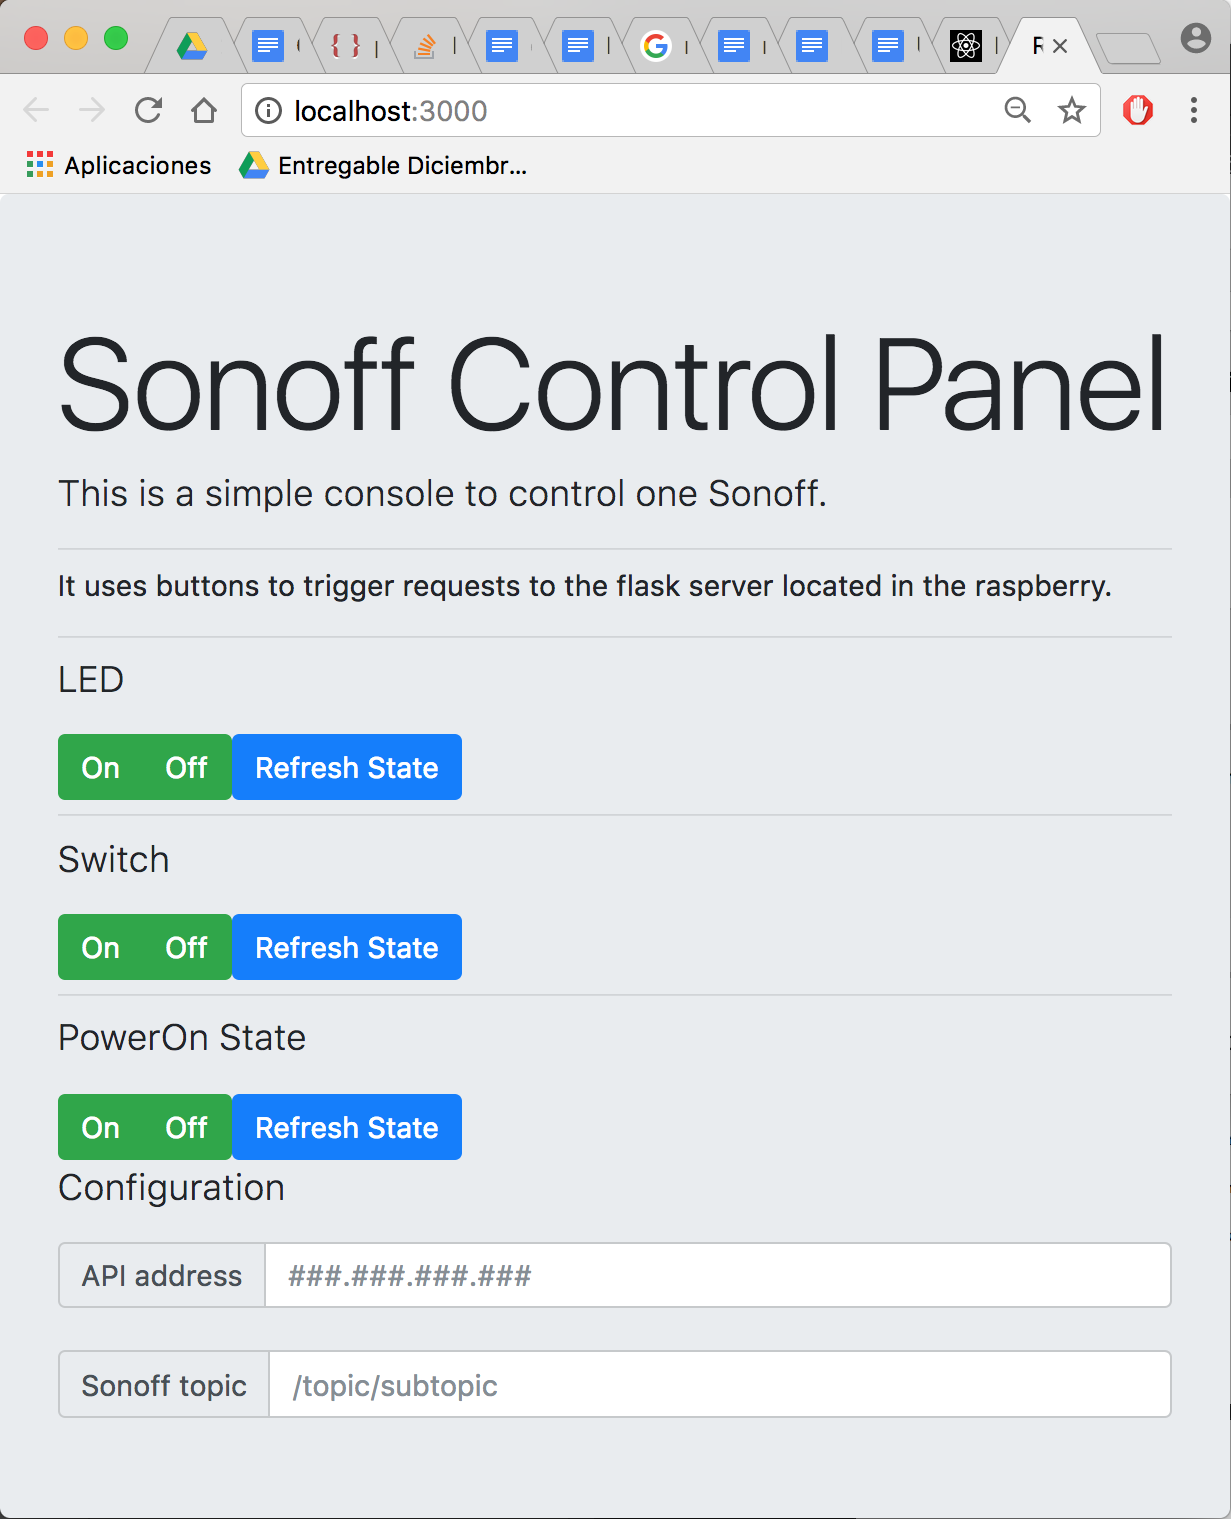
\includegraphics[width=0.5\textwidth, keepaspectratio]{images/vista-app-web}
  \caption{\textit{Vista de página principal provisoria.}}
  \label{fig:pag-prin-prov}
\end{figure}

En la figura~\qref{fig:pag-prin-prov} se puede observar los botones para prender y apagar tanto el LED como el relé, el último sirve para indicar el estado del relé cuando el Sonoff inicia. Todos los botones reflejan el estado actual del componente, actualizándose si el mismo cambia por un motivo externo a la misma aplicación (corte de luz, cambio de estado mediante otra sesión se la aplicación o mediante otra interfaz de usuario).

El código de la misma se puede observar bajo el anexo~\qref{anexo-app-web}


\paragraph{Aplicación Web y Móvil:}\

Para el desarrollo final se utilizaron las herramientas y librerías \lstinline[columns=fixed]{Auth0}~\cite{Auth0}, \lstinline[columns=fixed]{Phonegap}~\cite{Phonegap} y \lstinline[columns=fixed]{Android Studio}~\cite{AndroidStudio}.

Para la autenticación de la aplicación celular y web se utilizó la herramienta Auth0, ya que provee funcionalidades muy completas que no podrían haber sido implementadas debido a los tiempos manejados y siendo que no es este el foco del proyecto.
Esta herramienta terceriza el servicio de autentificación, pudiendo crearse usuarios propios del servicio o utilizando varias cuentas de otras aplicaciones, entre ellas Facebook, Github y Google.
El flujo de autenticación conlleva una redirección a una página brindada por Auth0, donde el usuario es identificado por alguno de los medios permitidos por la aplicación que solicita la autenticación. ~\qref{fig:auth0-flow}
Una vez autenticado el usuario, Auth0 redirige al usuario nuevamente hacia la aplicación, brindando información del usuario y un token que expira en un tiempo determinado para aumentar la seguridad.

\begin{figure}[H]
  \centering
  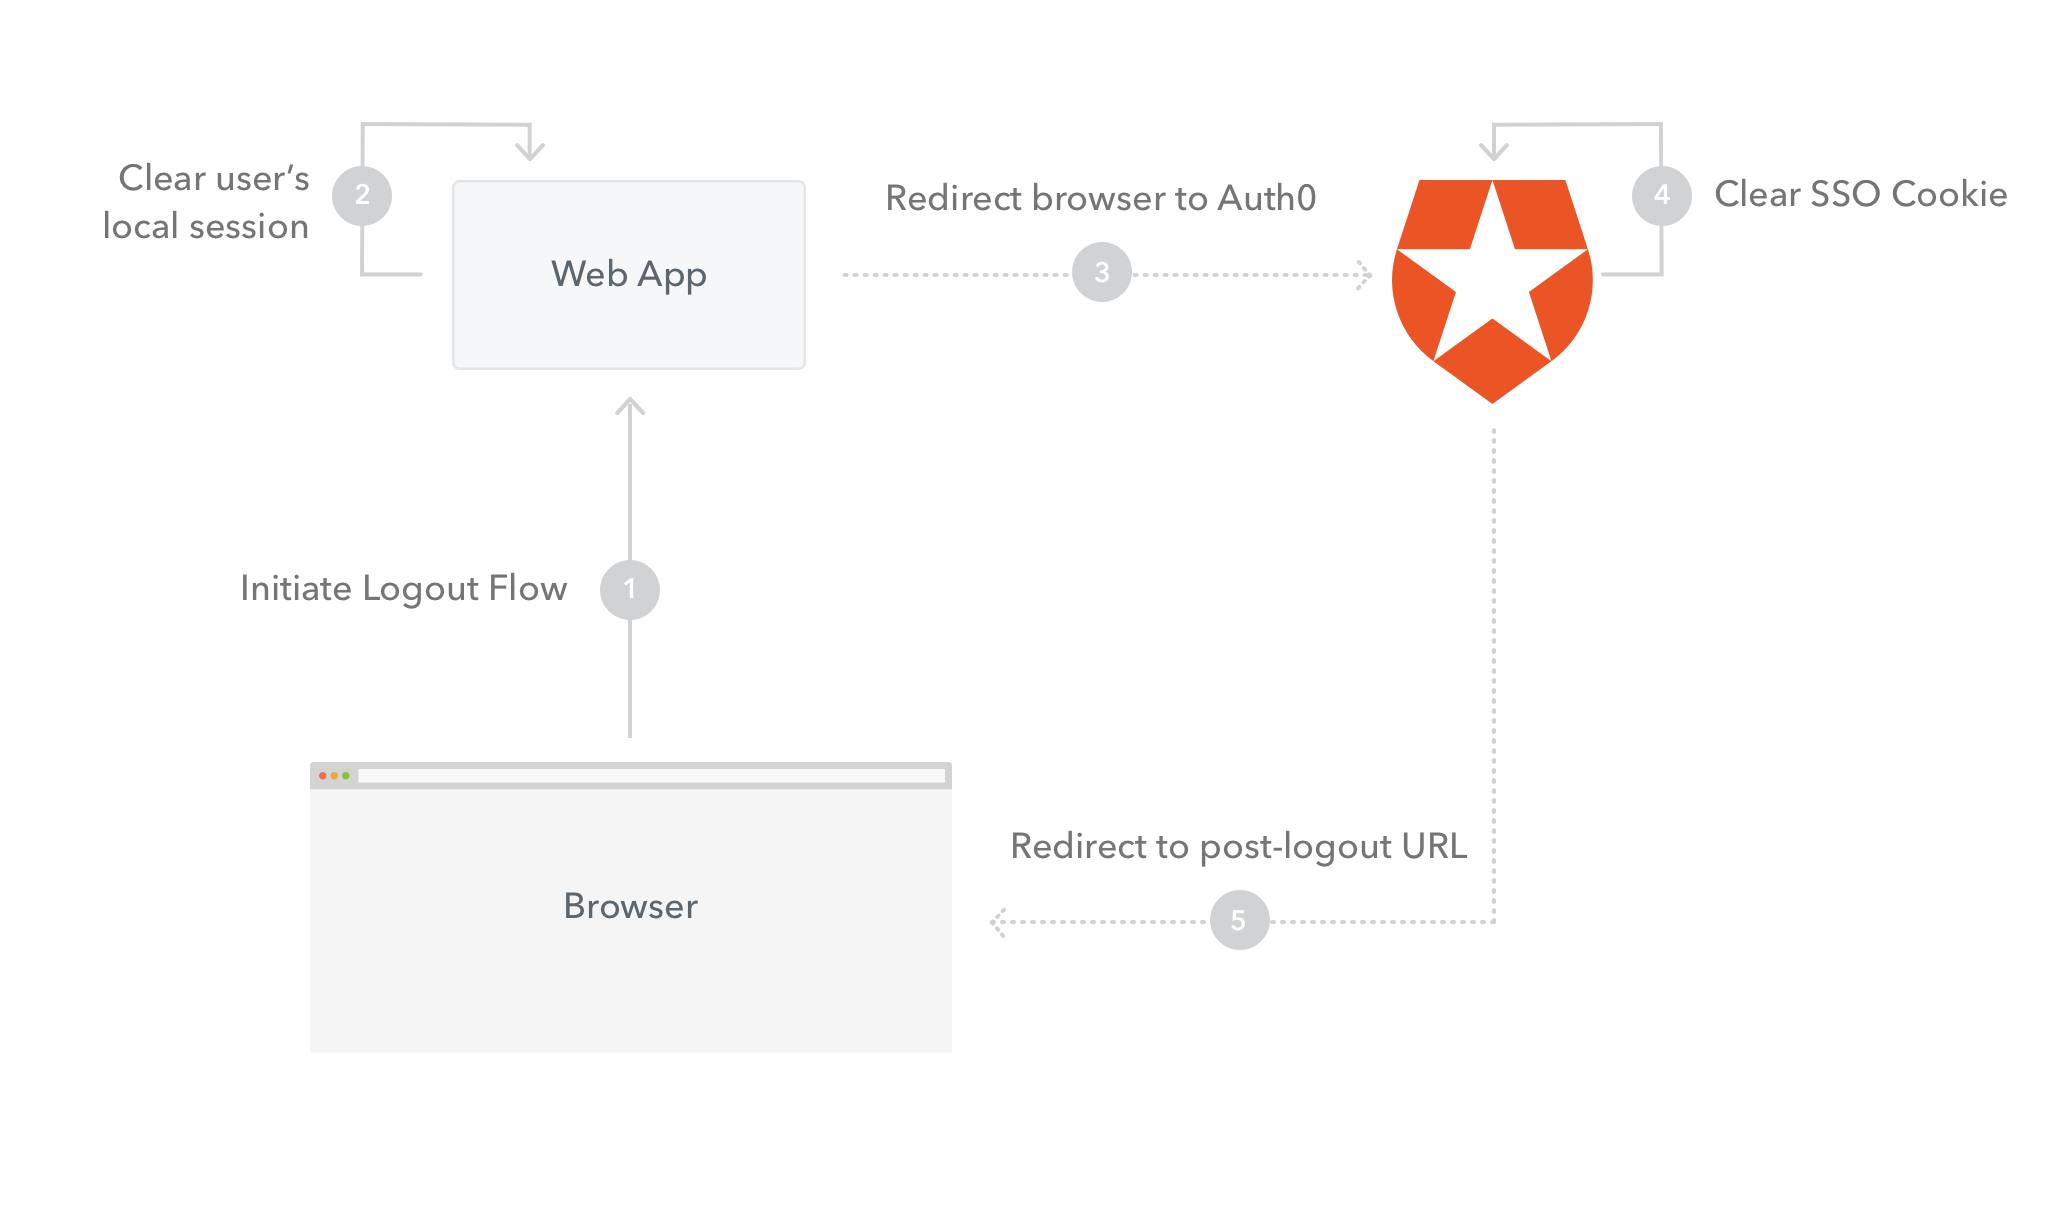
\includegraphics[width=0.5\textwidth, keepaspectratio]{images/auth0}
  \caption{\textit{Flujo de autenticación con Auth0.}}
  \label{fig:auth0-flow}
\end{figure}

Otras funciones interesantes que permite utilizar sin necesidad de ser implementadas son:

\begin{itemize}
  \item Recuperación de contraseña.
  \item Notificaciones vía mail de ingreso sospechoso.
  \item Validación de cuentas por medio de e-mail o mensaje de texto.
  \item Activación de autenticación de tres vías, utilizando aplicaciones como Google Authenticator o Authy.
\end{itemize}

El desarrollo se realizó con tecnologías web, permitiendo así que Phonegap compile las versiones web y móviles sin problemas, algunas configuraciones difieren en la configuración de la autenticación por parte de Auth0, ya que se realizan callbacks diferentes, siendo el de la aplicación móvil uno especial considerado por Auth0.
El resto de la aplicación funciona como se espera a pesar de la necesidad de ajustes de tamaño estéticos y de usabilidad debido a las diferencias proporcionales de las pantallas.
Para crear el proyecto en Phonegap se instala el paquete con la herramienta `npm`.

\begin{lstlisting}[language=bash]
  npm install -g phonegap
\end{lstlisting}

Luego se inicializa el proyecto con `phonegap create web\_app`, que crea el esqueleto del proyecto, que incluye entre los componentes más importantes: 
\begin{itemize}
  \item node\_modules: carpeta con los módulos de node instalados
  \item www: carpeta donde se contendrán los archivos de la página web.
  \item config.xml: archivo que contiene metadata de la aplicación así como librerías y plataformas que se han habilitado para el empaquetamiento.
\end{itemize}

Una vez agregado código en la carpeta www, se compila para la plataforma Android ejecutando:

\begin{lstlisting}[language=bash]
  phonegap build android
\end{lstlisting}

Y para la aplicación web:

\begin{lstlisting}[language=bash]
  phonegap build browser
\end{lstlisting}

Para poder ir visualizando los resultados del desarrollo, se serve la aplicación en un servidor local para desarrollar la versión web y emular un móvil Android gracias a Android Studio. 
Para levantar el servidor local basta con ejecutar \lstinline[columns=fixed]{phonegap serve}, levantando el servicio en el puerto \lstinline[columns=fixed]{3000}. En modo default cuenta con una configuración que permite la recarga automática ante cambios en el código que hicieron de esta la herramienta principal para el desarrollo de la aplicación.
A diferencia de la aplicación web, la aplicación móvil hizo necesaria la instalación del Android Studio para contar con el servicio de emulación, ya que no se contaban con móviles a disposición. Una vez instalado android studio se debe entrar al proyecto e inicializar una instancia de un celular, pudiéndose elegir entre múltiples modelos. Luego se debe seleccionar y descargar el sistema operativo, en nuestro caso utilizamos Android Oreo en Pixel 2.
Luego se compila y sube la aplicación corriendo el emulador y el comando \lstinline[columns=fixed]{phonegap run android}.

Antes de comenzar el desarrollo el código de la aplicación web, se realizó un bosquejo de este en Balsamic, que permite además de dibujar sencillamente las páginas, también permite definir links que funcionan como botones, cambiando las vistas para poder definir flujos intuitivos y determinar las páginas necesarias. Una vez planificada la estructura de la página se comenzó con la implementación práctica.

\begin{figure}[H]
  \centering
  \begin{subfigure}[b]{0.20\textwidth}
    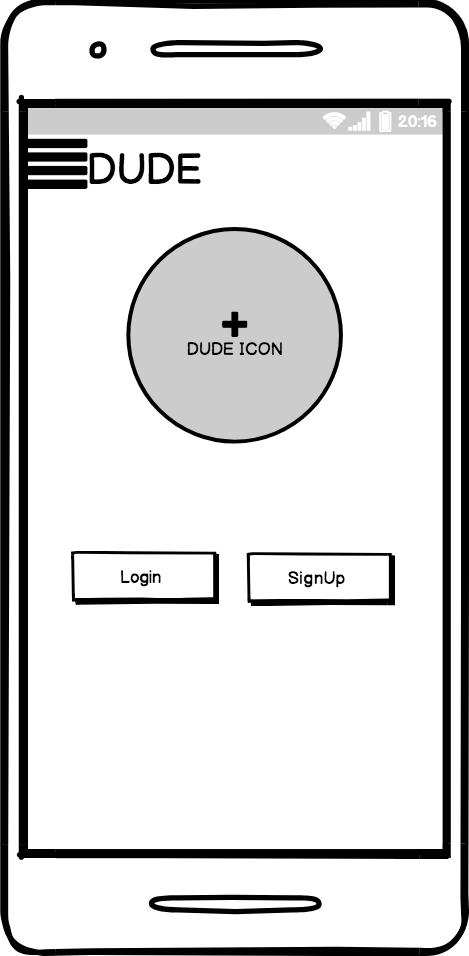
\includegraphics[width=\textwidth, keepaspectratio]{images/balsamiq01}
    \label{fig:balsamiq}
  \end{subfigure}
  %
  \begin{subfigure}[b]{0.20\textwidth}
    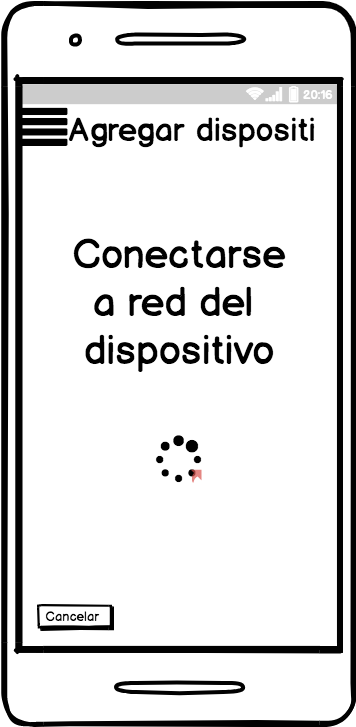
\includegraphics[width=\textwidth, keepaspectratio]{images/balsamiq02}
    \label{fig:balsamiq}
  \end{subfigure}
  %
  \begin{subfigure}[b]{0.20\textwidth}
    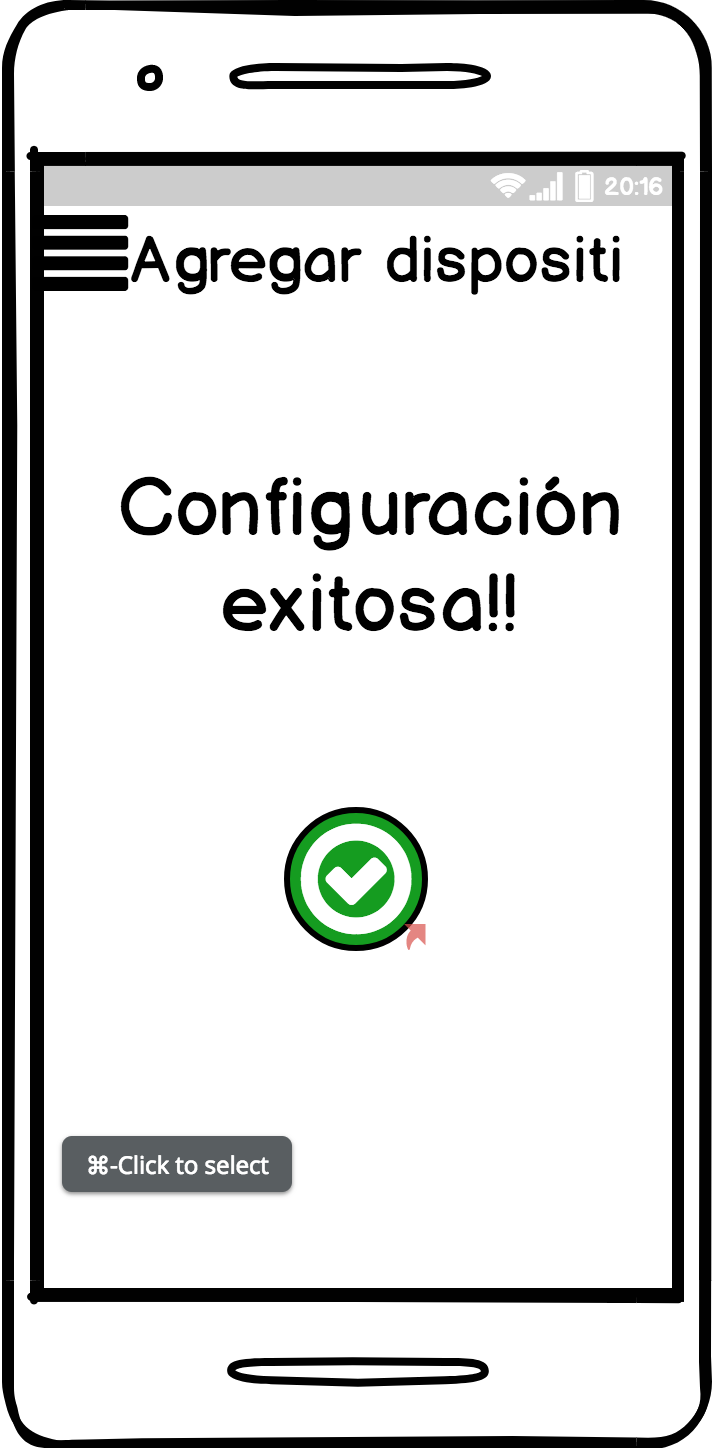
\includegraphics[width=\textwidth, keepaspectratio]{images/balsamiq03}
    \label{fig:balsamiq}
  \end{subfigure}
  %
  \begin{subfigure}[b]{0.20\textwidth}
    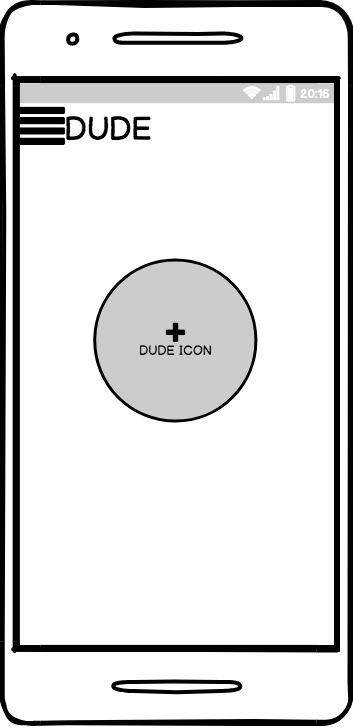
\includegraphics[width=\textwidth, keepaspectratio]{images/balsamiq04}
    \label{fig:balsamiq}
  \end{subfigure}
  %
  \begin{subfigure}[b]{0.20\textwidth}
    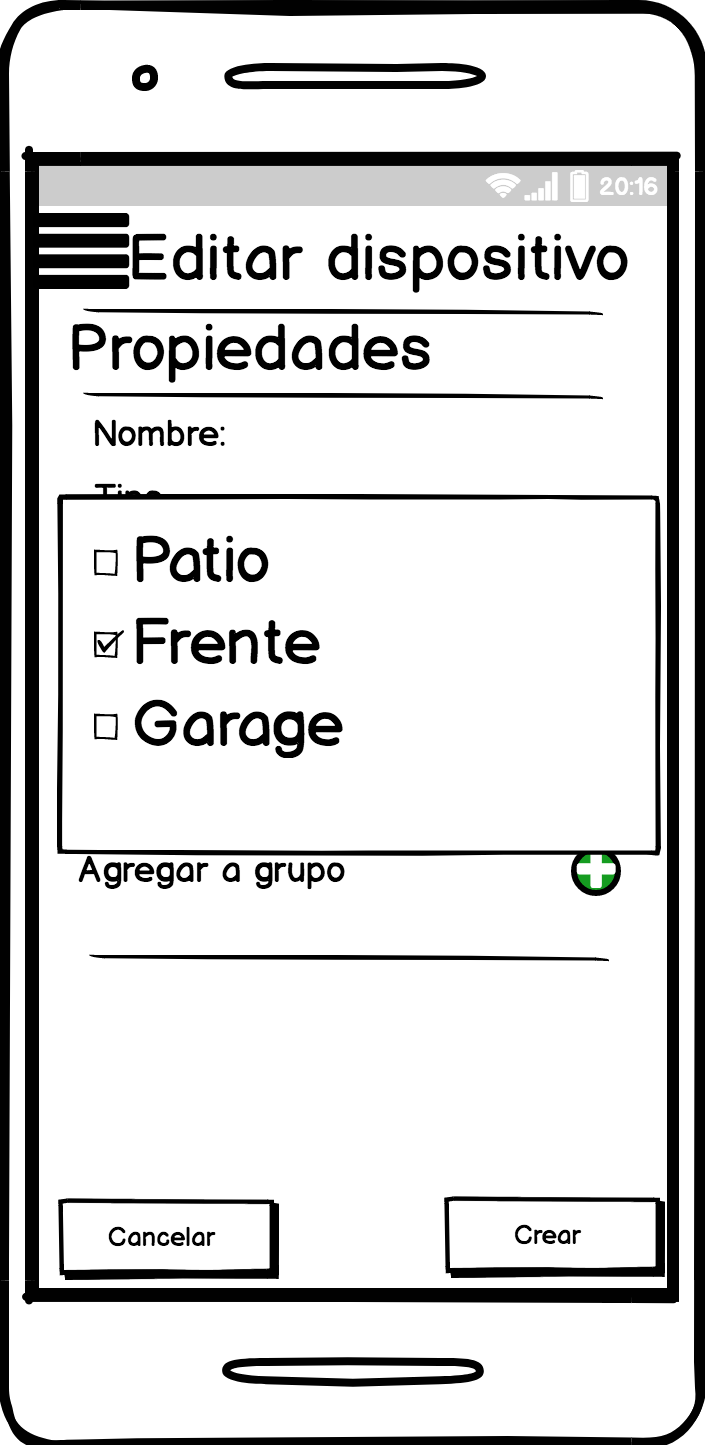
\includegraphics[width=\textwidth, keepaspectratio]{images/balsamiq05}
    \label{fig:balsamiq}
  \end{subfigure}
  %
  \begin{subfigure}[b]{0.20\textwidth}
    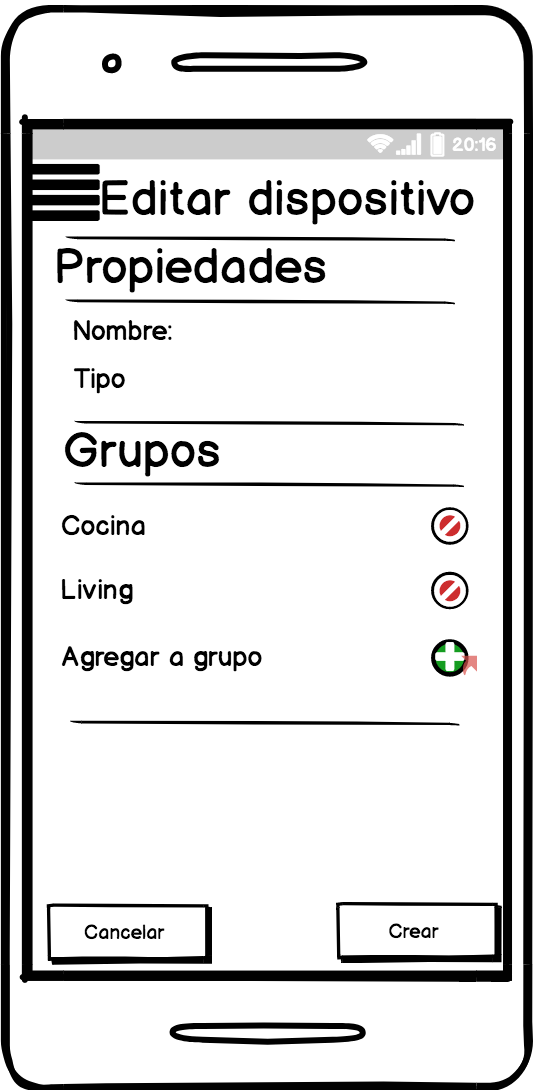
\includegraphics[width=\textwidth, keepaspectratio]{images/balsamiq06}
    \label{fig:balsamiq}
  \end{subfigure}
  %
  \begin{subfigure}[b]{0.20\textwidth}
    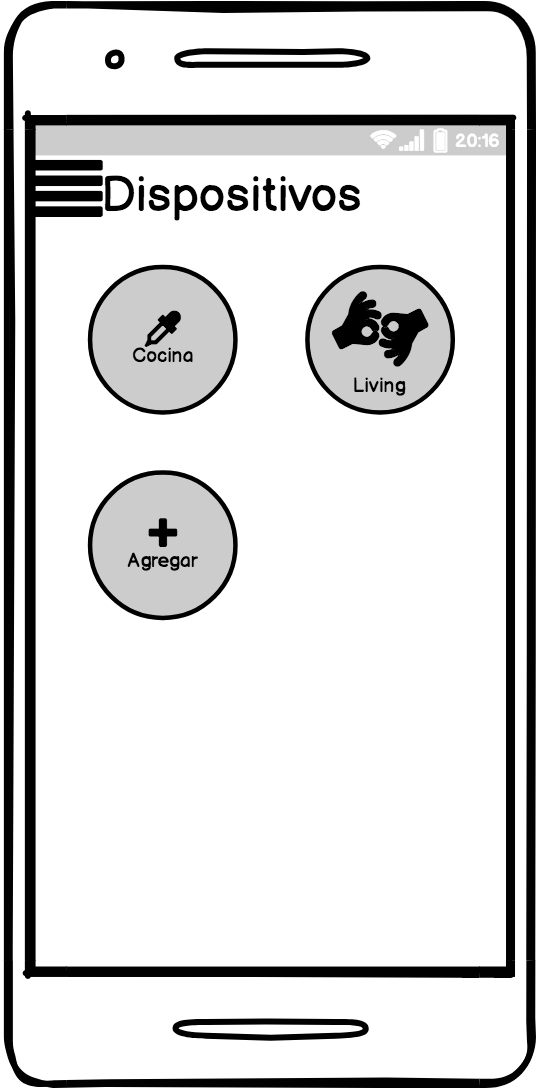
\includegraphics[width=\textwidth, keepaspectratio]{images/balsamiq07}
    \label{fig:balsamiq}
  \end{subfigure}
  %
  \begin{subfigure}[b]{0.20\textwidth}
    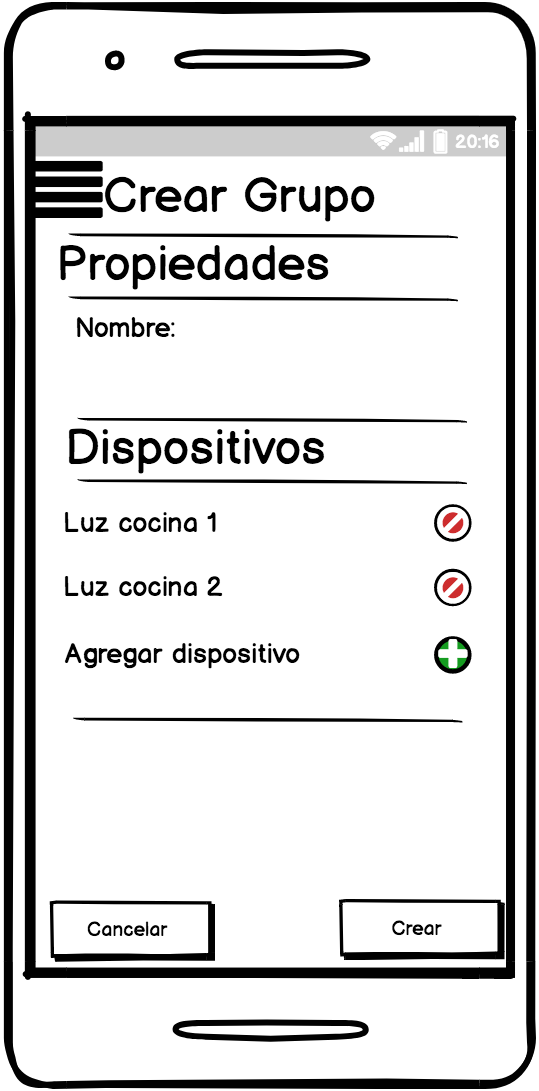
\includegraphics[width=\textwidth, keepaspectratio]{images/balsamiq08}
    \label{fig:balsamiq}
  \end{subfigure}
  %
  \begin{subfigure}[b]{0.20\textwidth}
    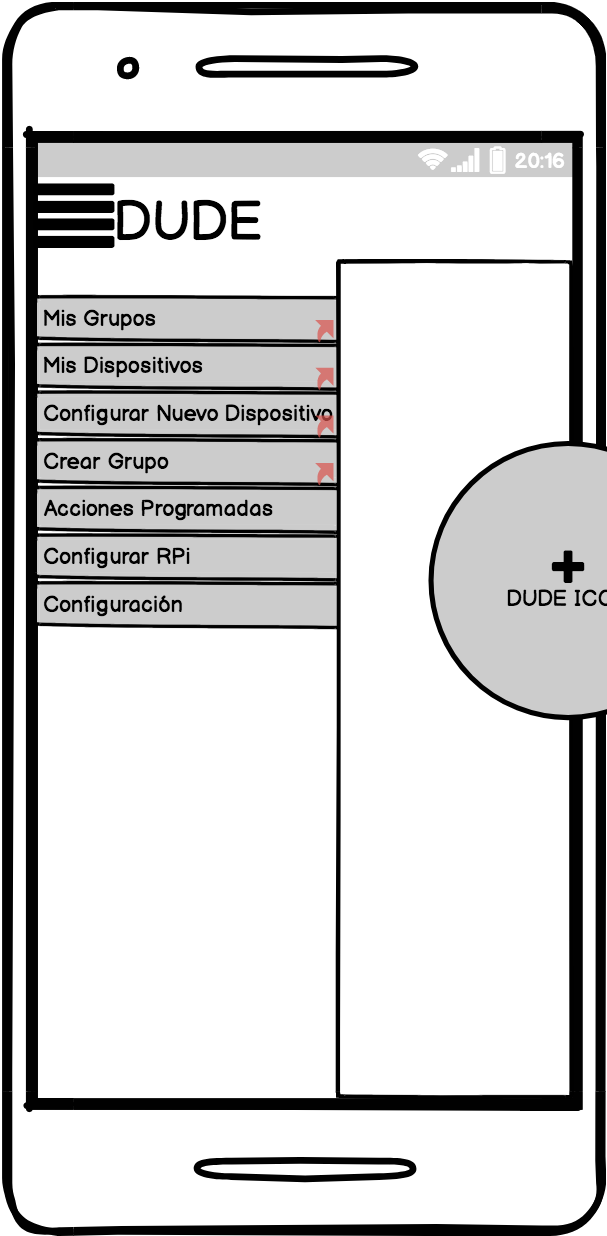
\includegraphics[width=\textwidth, keepaspectratio]{images/balsamiq09}
    \label{fig:balsamiq}
  \end{subfigure}
  %
  \begin{subfigure}[b]{0.20\textwidth}
    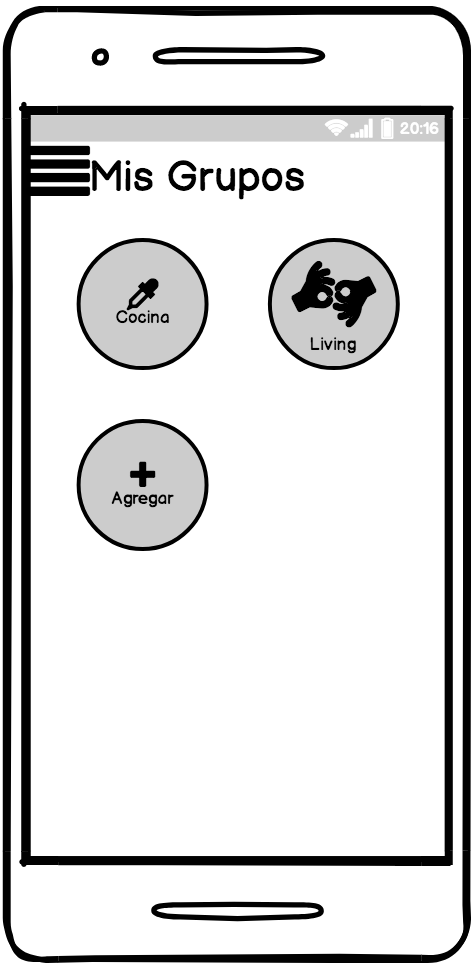
\includegraphics[width=\textwidth, keepaspectratio]{images/balsamiq10}
    \label{fig:balsamiq}
  \end{subfigure}
  %
  \begin{subfigure}[b]{0.20\textwidth}
    
\includegraphics[width=\textwidth, keepaspectratio]{images/balsamiq11}
    \label{fig:balsamiq}
  \end{subfigure}
\caption{\textit{Vistas creadas en Balsamiq.}}
\end{figure}


Para el desarrollo de la aplicación se decidió adquirir un template para no tener que invertir tiempo en la parte estética de la aplicación. Para la elección del mismo se tuvo en cuenta las librerías que utilizan y la adaptabilidad a versiones móviles.
El tema elegido fué MegaMobile de \lstinline[columns=fixed]{Enabled}~\cite{Enabled}, debido a su interfaz vistosa y el estilo de las barras laterales y botones, los cuales se adecuaban a las pantallas diseñadas en Balsamic.

\subparagraph{Librería jquery-cron:}\mbox{}\\
Debido a la utilización de cron del lado del servidor, es necesario traducir la hora, día, etc a la que el usuario quiere realizar el apagado y prendido de los dispositivos o de los grupos a el formato de cron. Para esto se utilizó una librería llamada \lstinline[columns=fixed]{jquery-cron} que simplifica esta tarea. La misma consiste en una interfaz muy simple, como se ve a continuación, que cambia el \lstinline[columns=fixed]{String} del cron generado dependiendo de lo que el usuario ingrese.
A su vez, \lstinline[columns=fixed]{jquery-cron} es complementada por \lstinline[columns=fixed]{jquery-gentleSelect} que decora los bordes de los selectores. ~\qref{fig:jquery-cron-selectors}

\begin{figure}[H]
  \centering
  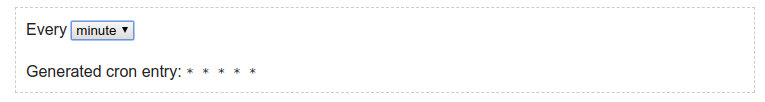
\includegraphics[width=\textwidth, keepaspectratio]{images/jquery-cron1}
  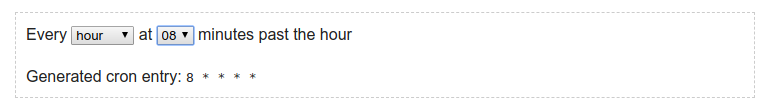
\includegraphics[width=\textwidth, keepaspectratio]{images/jquery-cron2}
  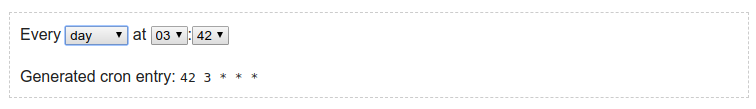
\includegraphics[width=\textwidth, keepaspectratio]{images/jquery-cron3}
  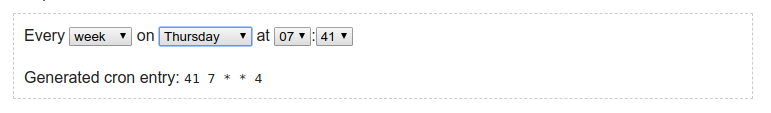
\includegraphics[width=\textwidth, keepaspectratio]{images/jquery-cron4}
  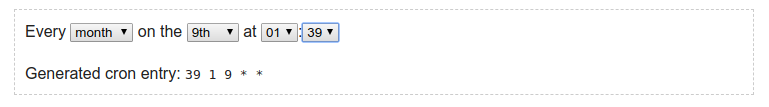
\includegraphics[width=\textwidth, keepaspectratio]{images/jquery-cron5}
  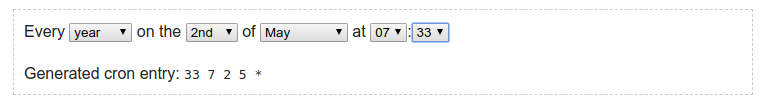
\includegraphics[width=\textwidth, keepaspectratio]{images/jquery-cron6}
  \caption{\textit{Selectores jquery-cron.}}
  \label{fig:jquery-cron-selectors}
\end{figure}

Se adaptó esta librería creando un fork del proyecto para que todos los nombres de las opciones y textos queden en español, esta modificación quedó disponible para la utilización de la comunidad.
Para usar esta librería alcanza con tener dos divs, uno para el scheduler y otro para texto resultante. El margen izquierdo del div de texto es negativo para que no aparezca en la pantalla, dado que el cron debe ser transparente para el usuario.

\begin{lstlisting}[language=python]
<div id="selector_scheduler"></div>

<div class='example-text' style="margin: 0px 0px 0px -40%;" id='example1-val'></div>
\end{lstlisting}

Se debe cargar la librería antes de usarla, junto con \lstinline[columns=fixed]{jquery-gentleSelect}.

\begin{lstlisting}[language=python]
<script type="text/javascript" src="js/jquery-cron.js"></script>
<script type="text/javascript" src="js/jquery-gentleSelect.js"></script>
\end{lstlisting}

Luego, se crea la interfaz:

\begin{lstlisting}[language=python]
$('#selector_scheduler').cron({
          initial: "42 3 * * 5",
          onChange: function() {
              $('#example1-val').text($(this).cron("value"))
          },
          useGentleSelect: true
      })
\end{lstlisting}

\lstinline[columns=fixed]{Initial} es el valor inicial que toma el scheduler. Onchange toma una función para ejecutar cuando el usuario selecciona un nuevo valor en alguno de los selectores. Lo que hace la función es traducir lo que el usuario eligió y setearlo en el div de texto. \lstinline[columns=fixed]{UseGentleSelect} se pone en true para habilitar el uso de la librería \lstinline[columns=fixed]{jquery-gentleSelect}.


\subparagraph{Interfaz móvil y web}\mbox{}\mbox{}\\
Cuando el usuario abre por primera vez la aplicación, solo tiene la posibilidad de iniciar sesión.~\qref{fig:app-movil-home} Esto se realiza mediante el servicio autenticación \lstinline[columns=fixed]{Auth0}. Si no se cuenta con un token de autorización no expirado, la aplicación requerirá que el usuario se identifique.

\begin{figure}[H]
  \centering
  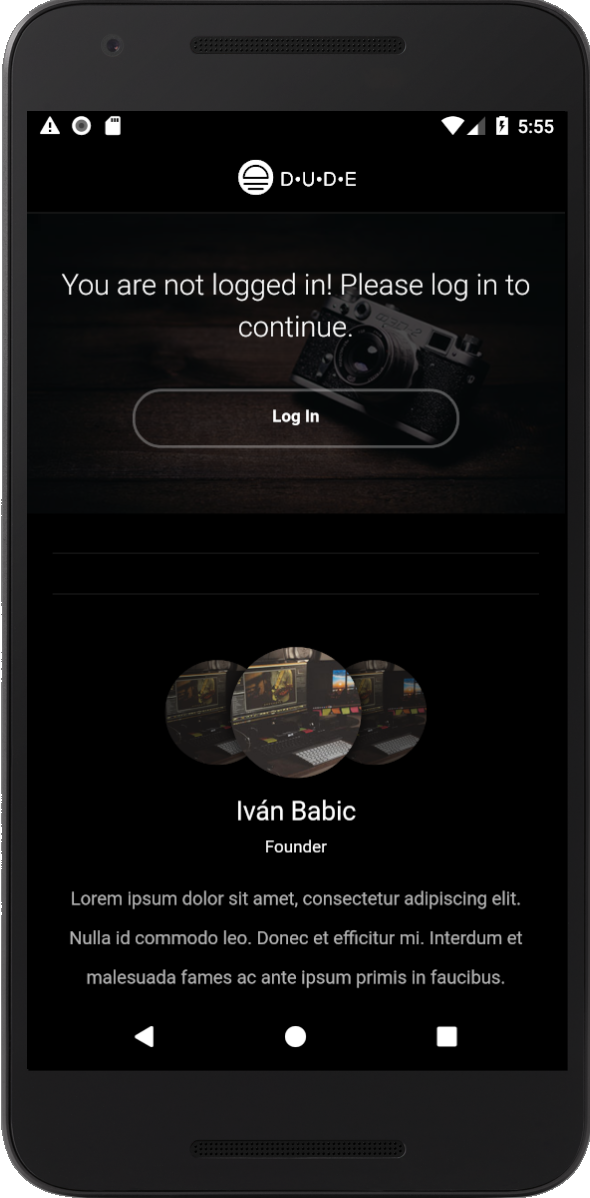
\includegraphics[width=0.2\textwidth, keepaspectratio]{images/app-movil-home}
  \caption{\textit{Página de inicio.}}
  \label{fig:app-movil-home}
\end{figure}

Una vez que se presiona el botón de LogIn, este lleva al servicio de google Auth0 para que el usuario pueda autenticarse. ~\qref{fig:app-movil-home}


\begin{figure}[H]
  \centering
  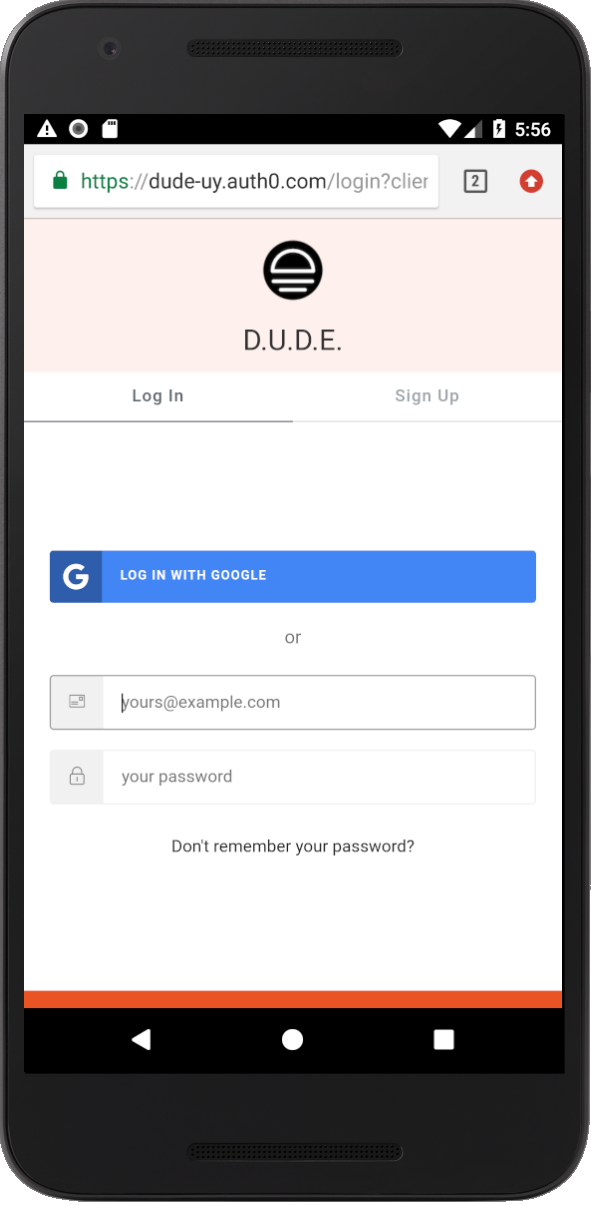
\includegraphics[width=0.2\textwidth, keepaspectratio]{images/app-movil-auth0}
  \caption{\textit{D.U.D.E. Auth0 Log In}}
  \label{fig:app-movil-auth0}
\end{figure}

Una vez que el usuario rellena sus datos y logra iniciar su sesión, la aplicación retorna con sesión iniciada, y checkea que se cuente con la configuración del Raspberry Pi.
En caso de que no esté configurado, se muestra la interfaz de configuración~\qref{fig:app-web-get-raspberry-configuration}, la cual permite ingresar la IP del Raspberry y al oprimir el botón enviarle un request de la configuración. Es totalmente necesaria la conexión entre dispositivo y raspberry para el funcionamiento de la aplicación, ya que es ahí donde se encuentra la base de datos con la información de dispositivos, y es sólo a travéz del dispositivo central que se puede interactuar con los demás dipositivos configurados.

\begin{figure}[H]
  \centering
  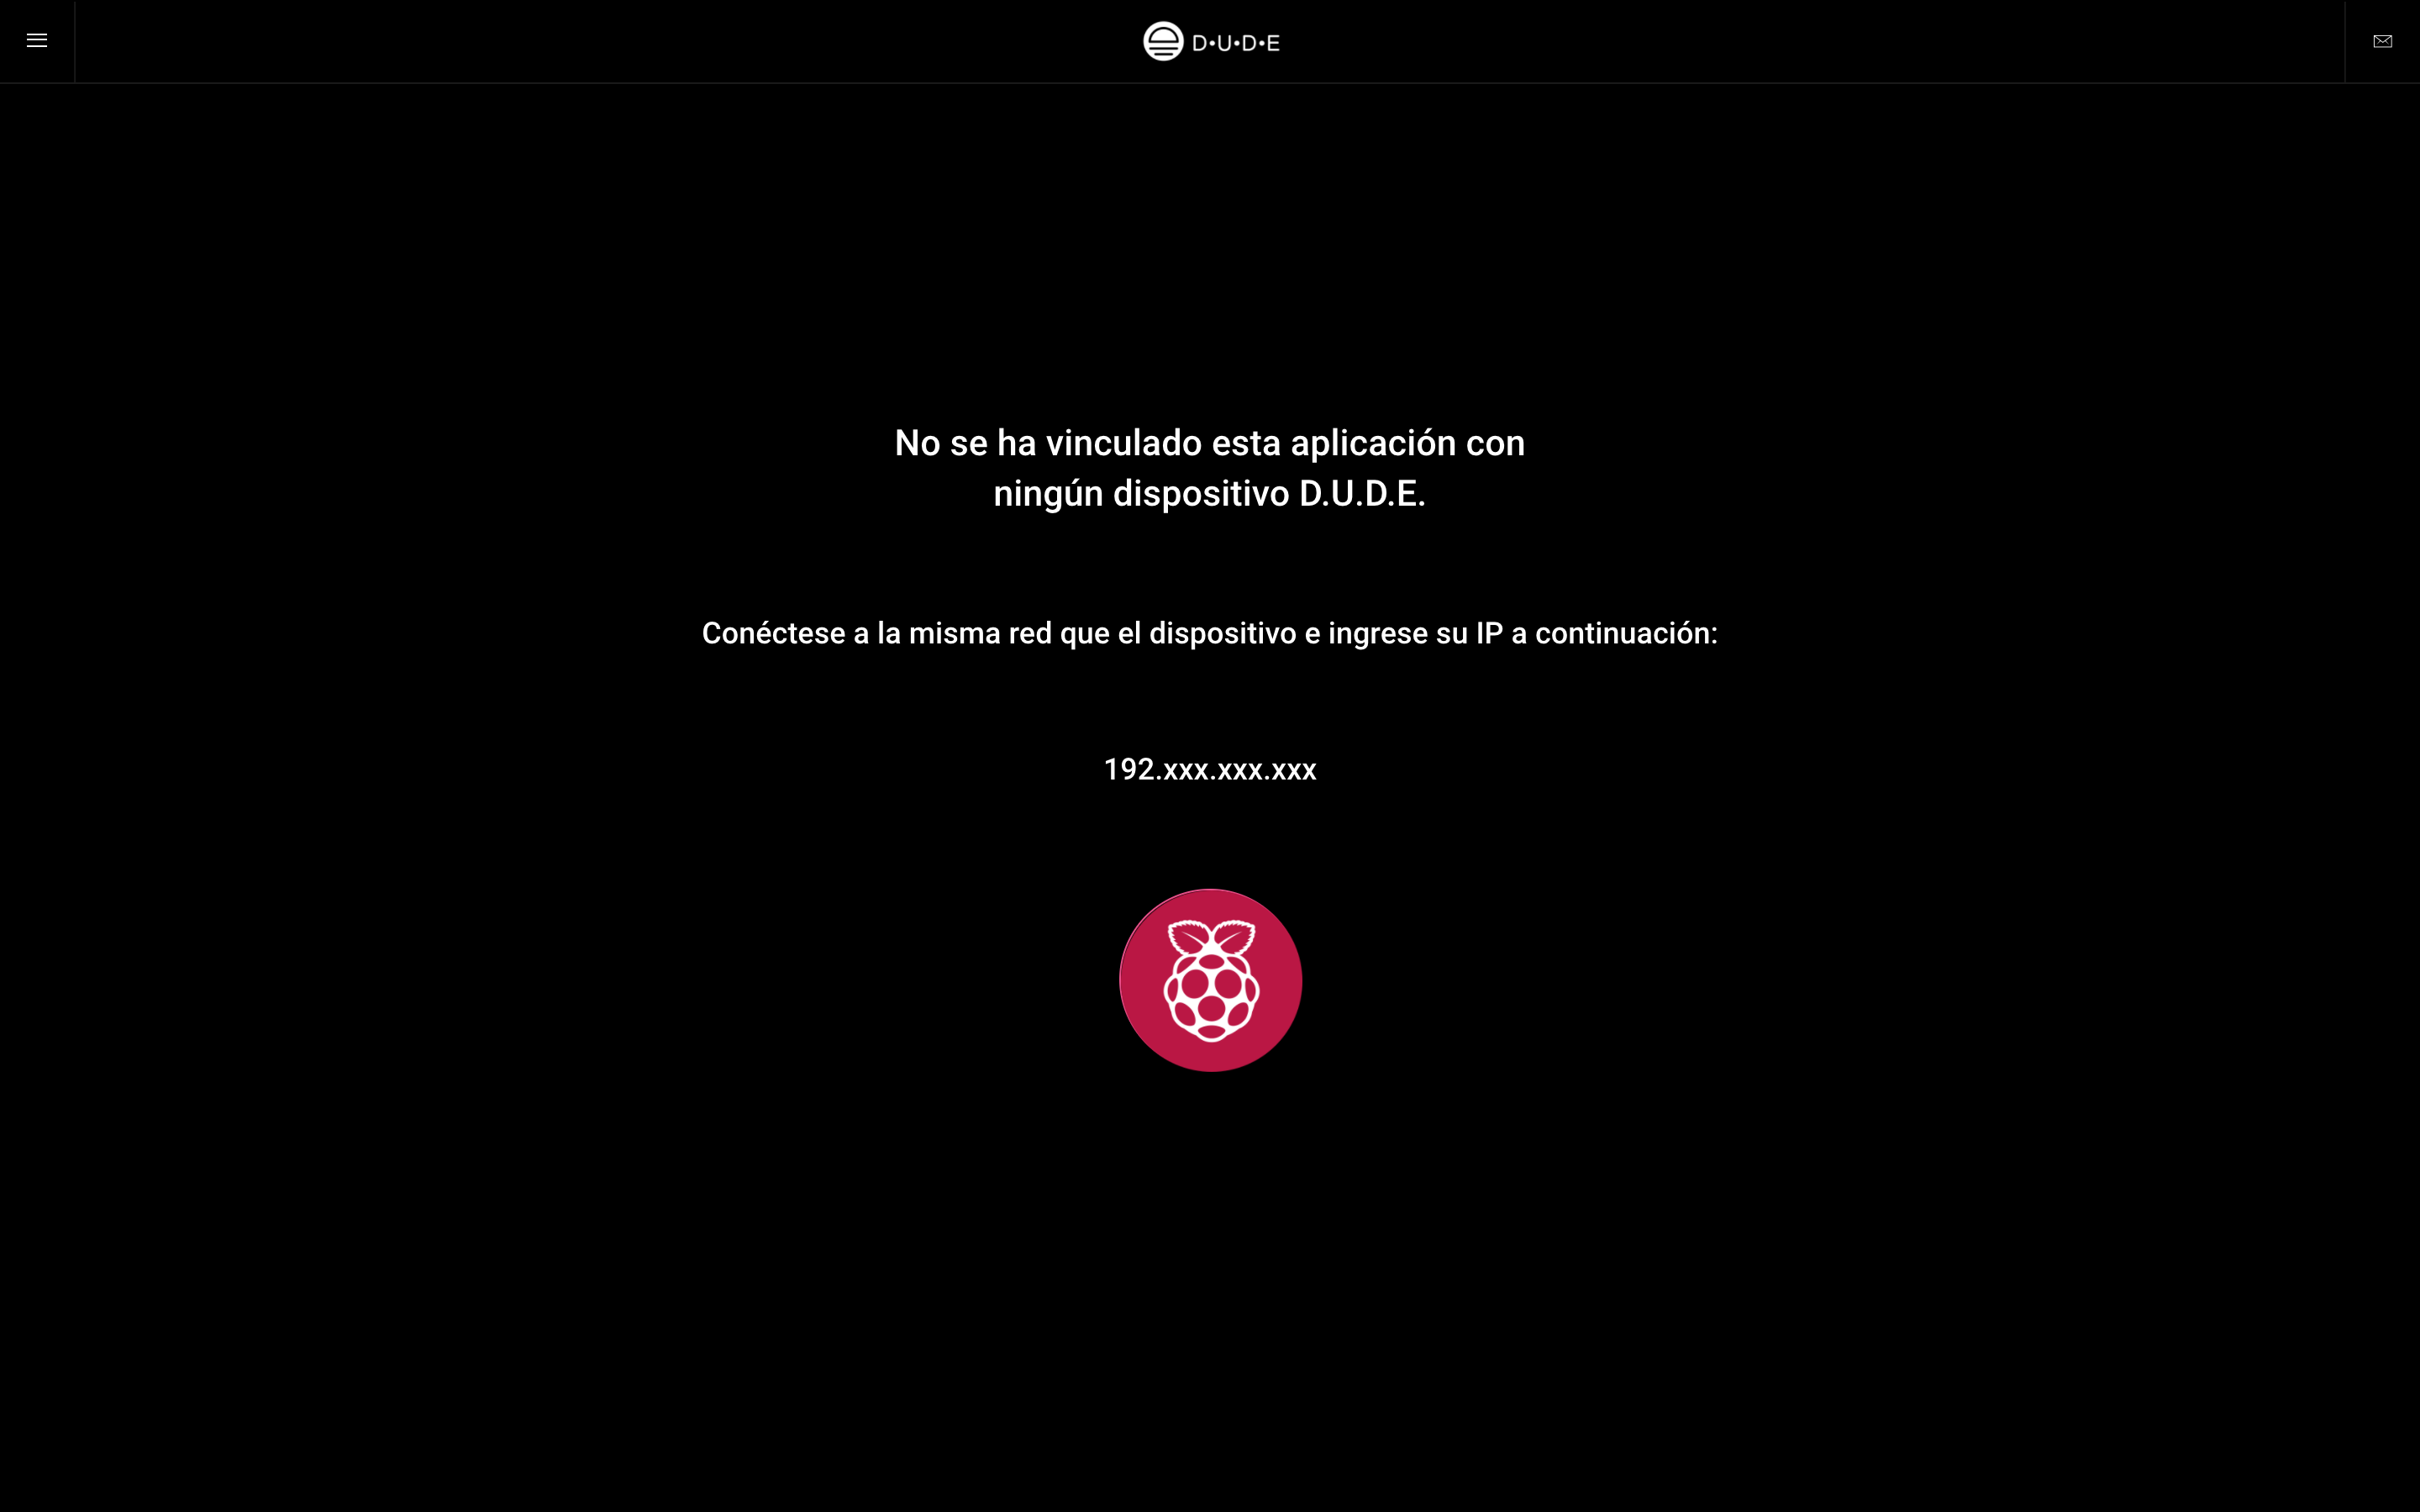
\includegraphics[width=0.6\textwidth, keepaspectratio]{images/app-web-get-raspberry-configuration}
  \caption{\textit{Página de configuración de dispositivo central.}}
  \label{fig:app-web-get-raspberry-configuration}
\end{figure}

Si ya se contaba con esta configuración, o luego de realizarla, se vuelve a la página principal. Aunque en este caso se cuenta con un mensaje que indica que la sesión, un botón para salir de ésta y un ícono en la esquina superior izquierda.~\qref{fig:app-movil-login-success}

\begin{figure}[H]
  \centering
  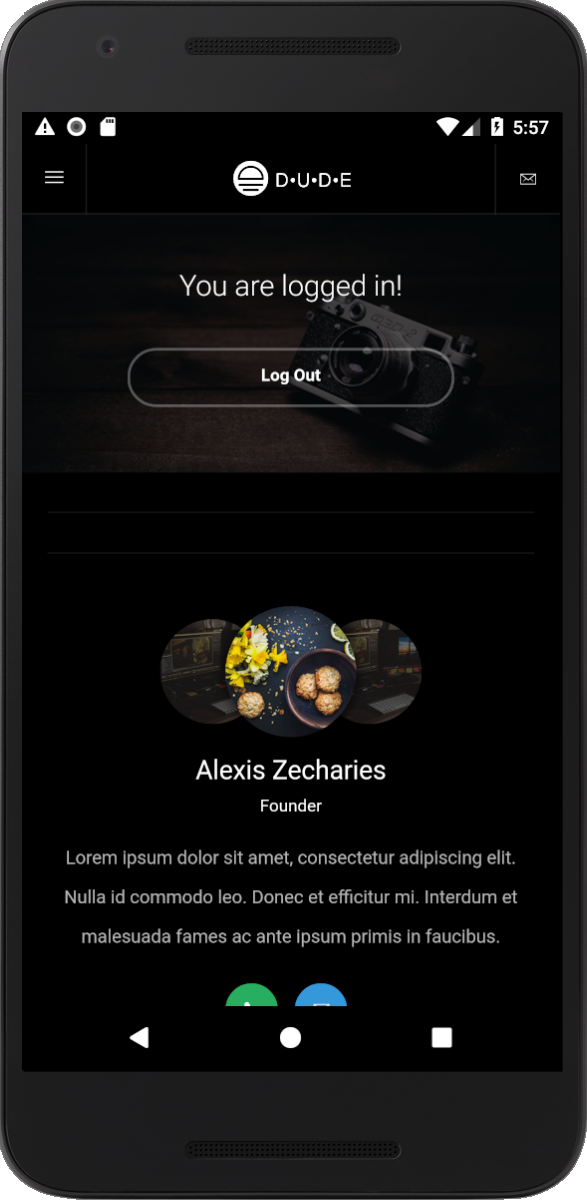
\includegraphics[width=0.2\textwidth, keepaspectratio]{images/app-movil-login-success}
  \caption{\textit{Página de inicio con sesión iniciada.}}
  \label{fig:app-movil-login-success}
\end{figure}

Al presionar este ícono, se desliza la barra lateral desde la izquierda. Esta contiene todas las funciones del sistema: 

\begin{itemize}
  \item Mis dispositivos
  \item Mis grupos
  \item Acciones programadas
    \begin{itemize}
      \item Dispositivo
      \item Grupo
    \end{itemize}
  \item Agregar entidad
    \begin{itemize}
      \item Dispositivo
      \item Grupo
    \end{itemize}
  \item Editar entidad
    \begin{itemize}
      \item Dispositivo
      \item Grupo
    \end{itemize}
  \item Configuración.
\end{itemize}

Al seleccionar \lstinline[columns=fixed]{Acciones programadas}, \lstinline[columns=fixed]{Agregar entidad} o \lstinline[columns=fixed]{Editar entidad} se abre un submenú en cada una que posibilita realizar estas acciones para dispositivos o para grupos.~\qref{fig:app-movil-sidebar}

\begin{figure}[H]
  \centering

  \begin{subfigure}[b]{0.2\textwidth}
    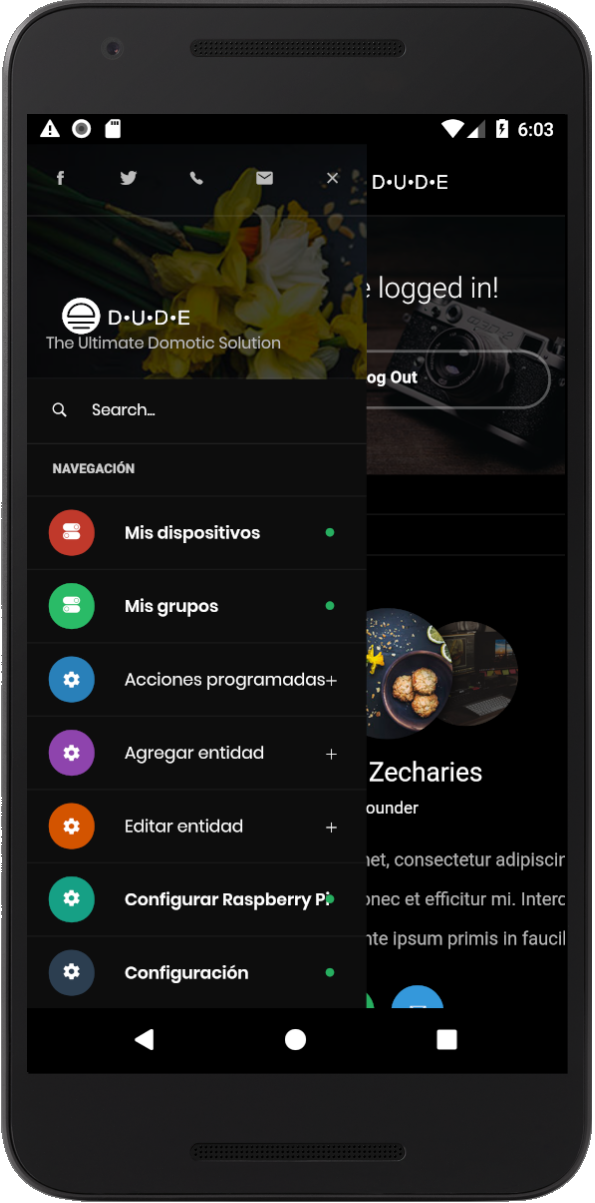
\includegraphics[width=\textwidth, keepaspectratio]{images/app-movil-sidebar}
    \caption{\textit{Funciones.}}
    \label{fig:app-movil-sidebar}
  \end{subfigure}
  %
  \begin{subfigure}[b]{0.2\textwidth}
    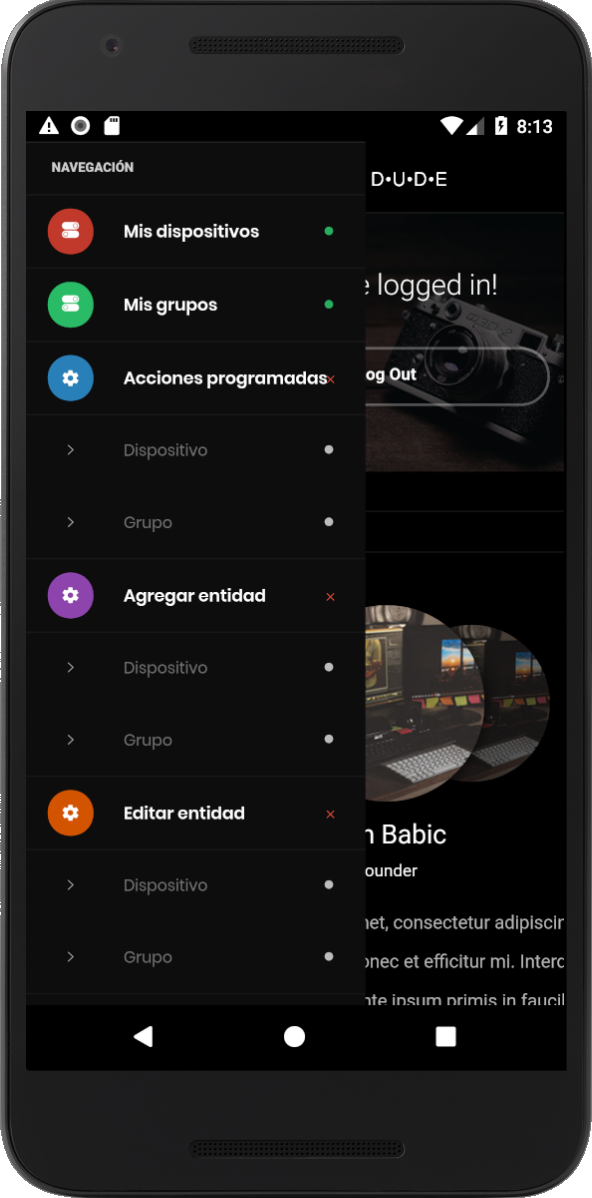
\includegraphics[width=\textwidth, keepaspectratio]{images/app-movil-sidebar-open}
    \caption{\textit{Opc. expandidas.}}
    \label{fig:app-movil-sidebar-open}
  \end{subfigure}

\caption{\textit{Vistas de barra lateral.}}
\end{figure}

\subparagraph{Funciones del sistema}\mbox{}\mbox{}\\

\textbf{Mis dispositivos}\\
Vista que permite modificar el estado de un dispositivo previamente agregado, la lista información de dispositivos es obtenida desde el Raspberry. se muestra un ícono de una lámpara apagada o prendida dependiendo del estado actual del dispositivo. Al presionar el botón con la bombilla se envía la orden al dispositivo central, quien publica la orden y cambia el estado en la base de datos.~\qref{fig:app-movil-choose-device}

\begin{figure}[H]
  \centering
  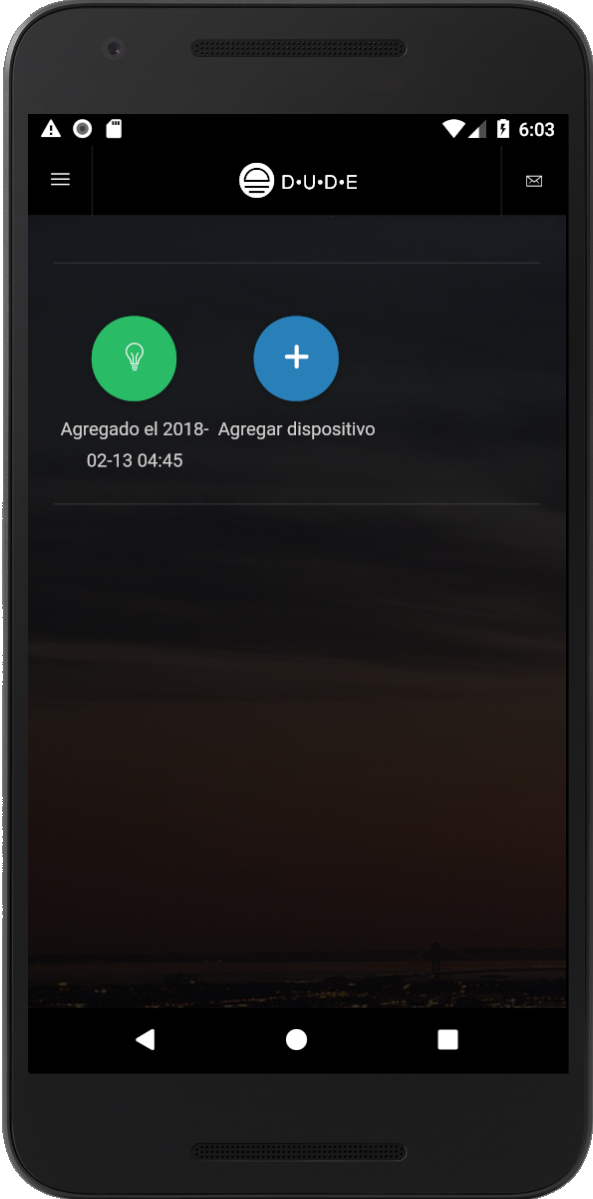
\includegraphics[width=0.2\textwidth, keepaspectratio]{images/app-movil-choose-device}
  \caption{\textit{Cambiar estado de dispositivo.}}
  \label{fig:app-movil-choose-device}
\end{figure}

\textbf{Mis grupos}\\
Vista que permite modificar el estado de un grupo existente. Ya que estos no tienen un estado de prendido o apagado porque los dispositivos pueden encontrarse en ambos estados aunque pertenezcan al mismo grupo, se le da la opción al usuario de cambiar de estado a todos los dispositivos del grupo mediante dos botones, uno con una bombilla apagada y otro con una bombilla prendida.~\qref{fig:app-movil-control-group}

\begin{figure}[H]
  \centering
  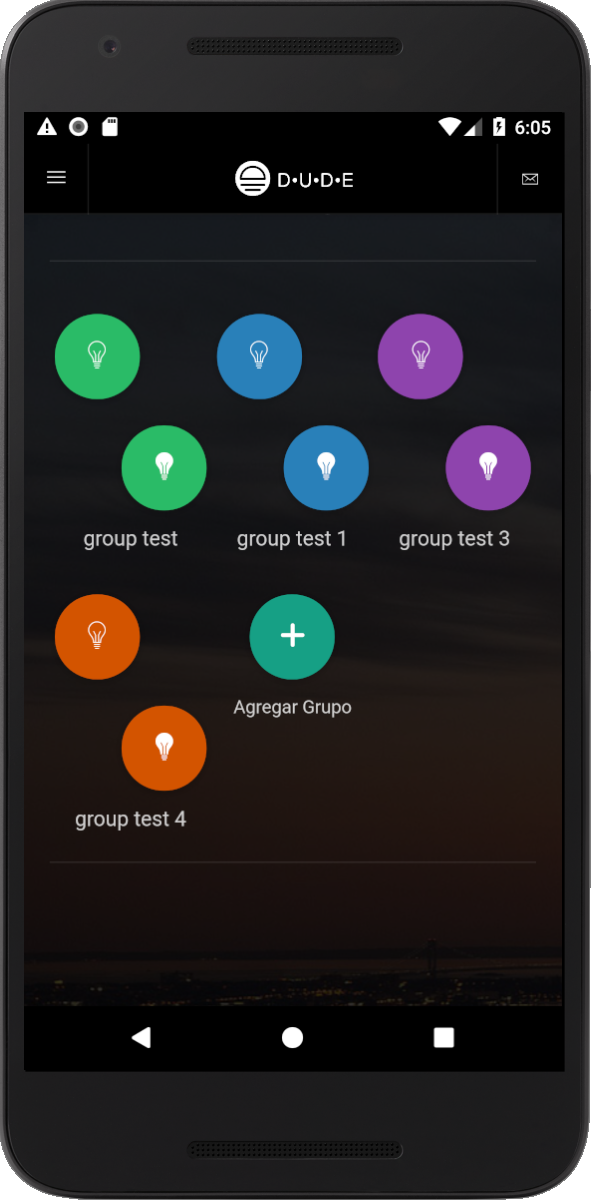
\includegraphics[width=0.2\textwidth, keepaspectratio]{images/app-movil-control-group}
  \caption{\textit{Cambiar estado de grupo.}}
  \label{fig:app-movil-control-group}
\end{figure}


\textbf{Elegir dispositivo}\\
En este las funciones \lstinline[columns=fixed]{Acciones programadas} y \lstinline[columns=fixed]{Editar entidad} se debe elegir el grupo o dispositivo al que se quiere programar una acción o editar. Esto se logra con las siguientes vistas.~\qref{fig:app-movil-choose-device}
\begin{figure}[H]
  \centering

  \begin{subfigure}[b]{0.2\textwidth}
    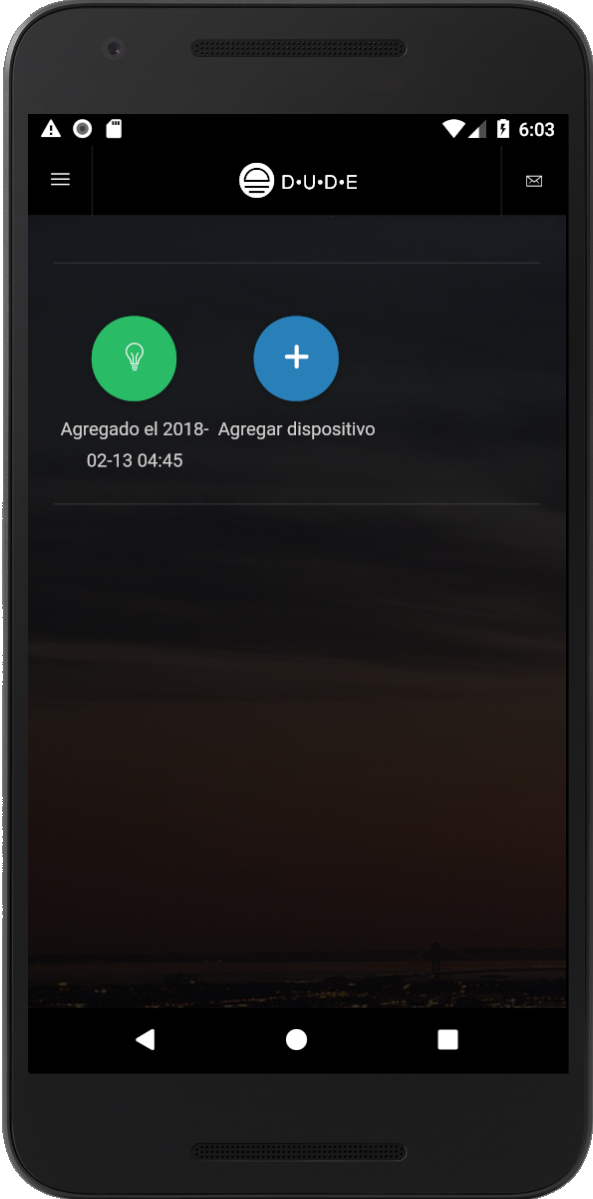
\includegraphics[width=\textwidth, keepaspectratio]{images/app-movil-choose-device}
    \caption{\textit{Dispositivo.}}
    \label{fig:app-movil-choose-device}
  \end{subfigure}
  %
  \begin{subfigure}[b]{0.6\textwidth}
    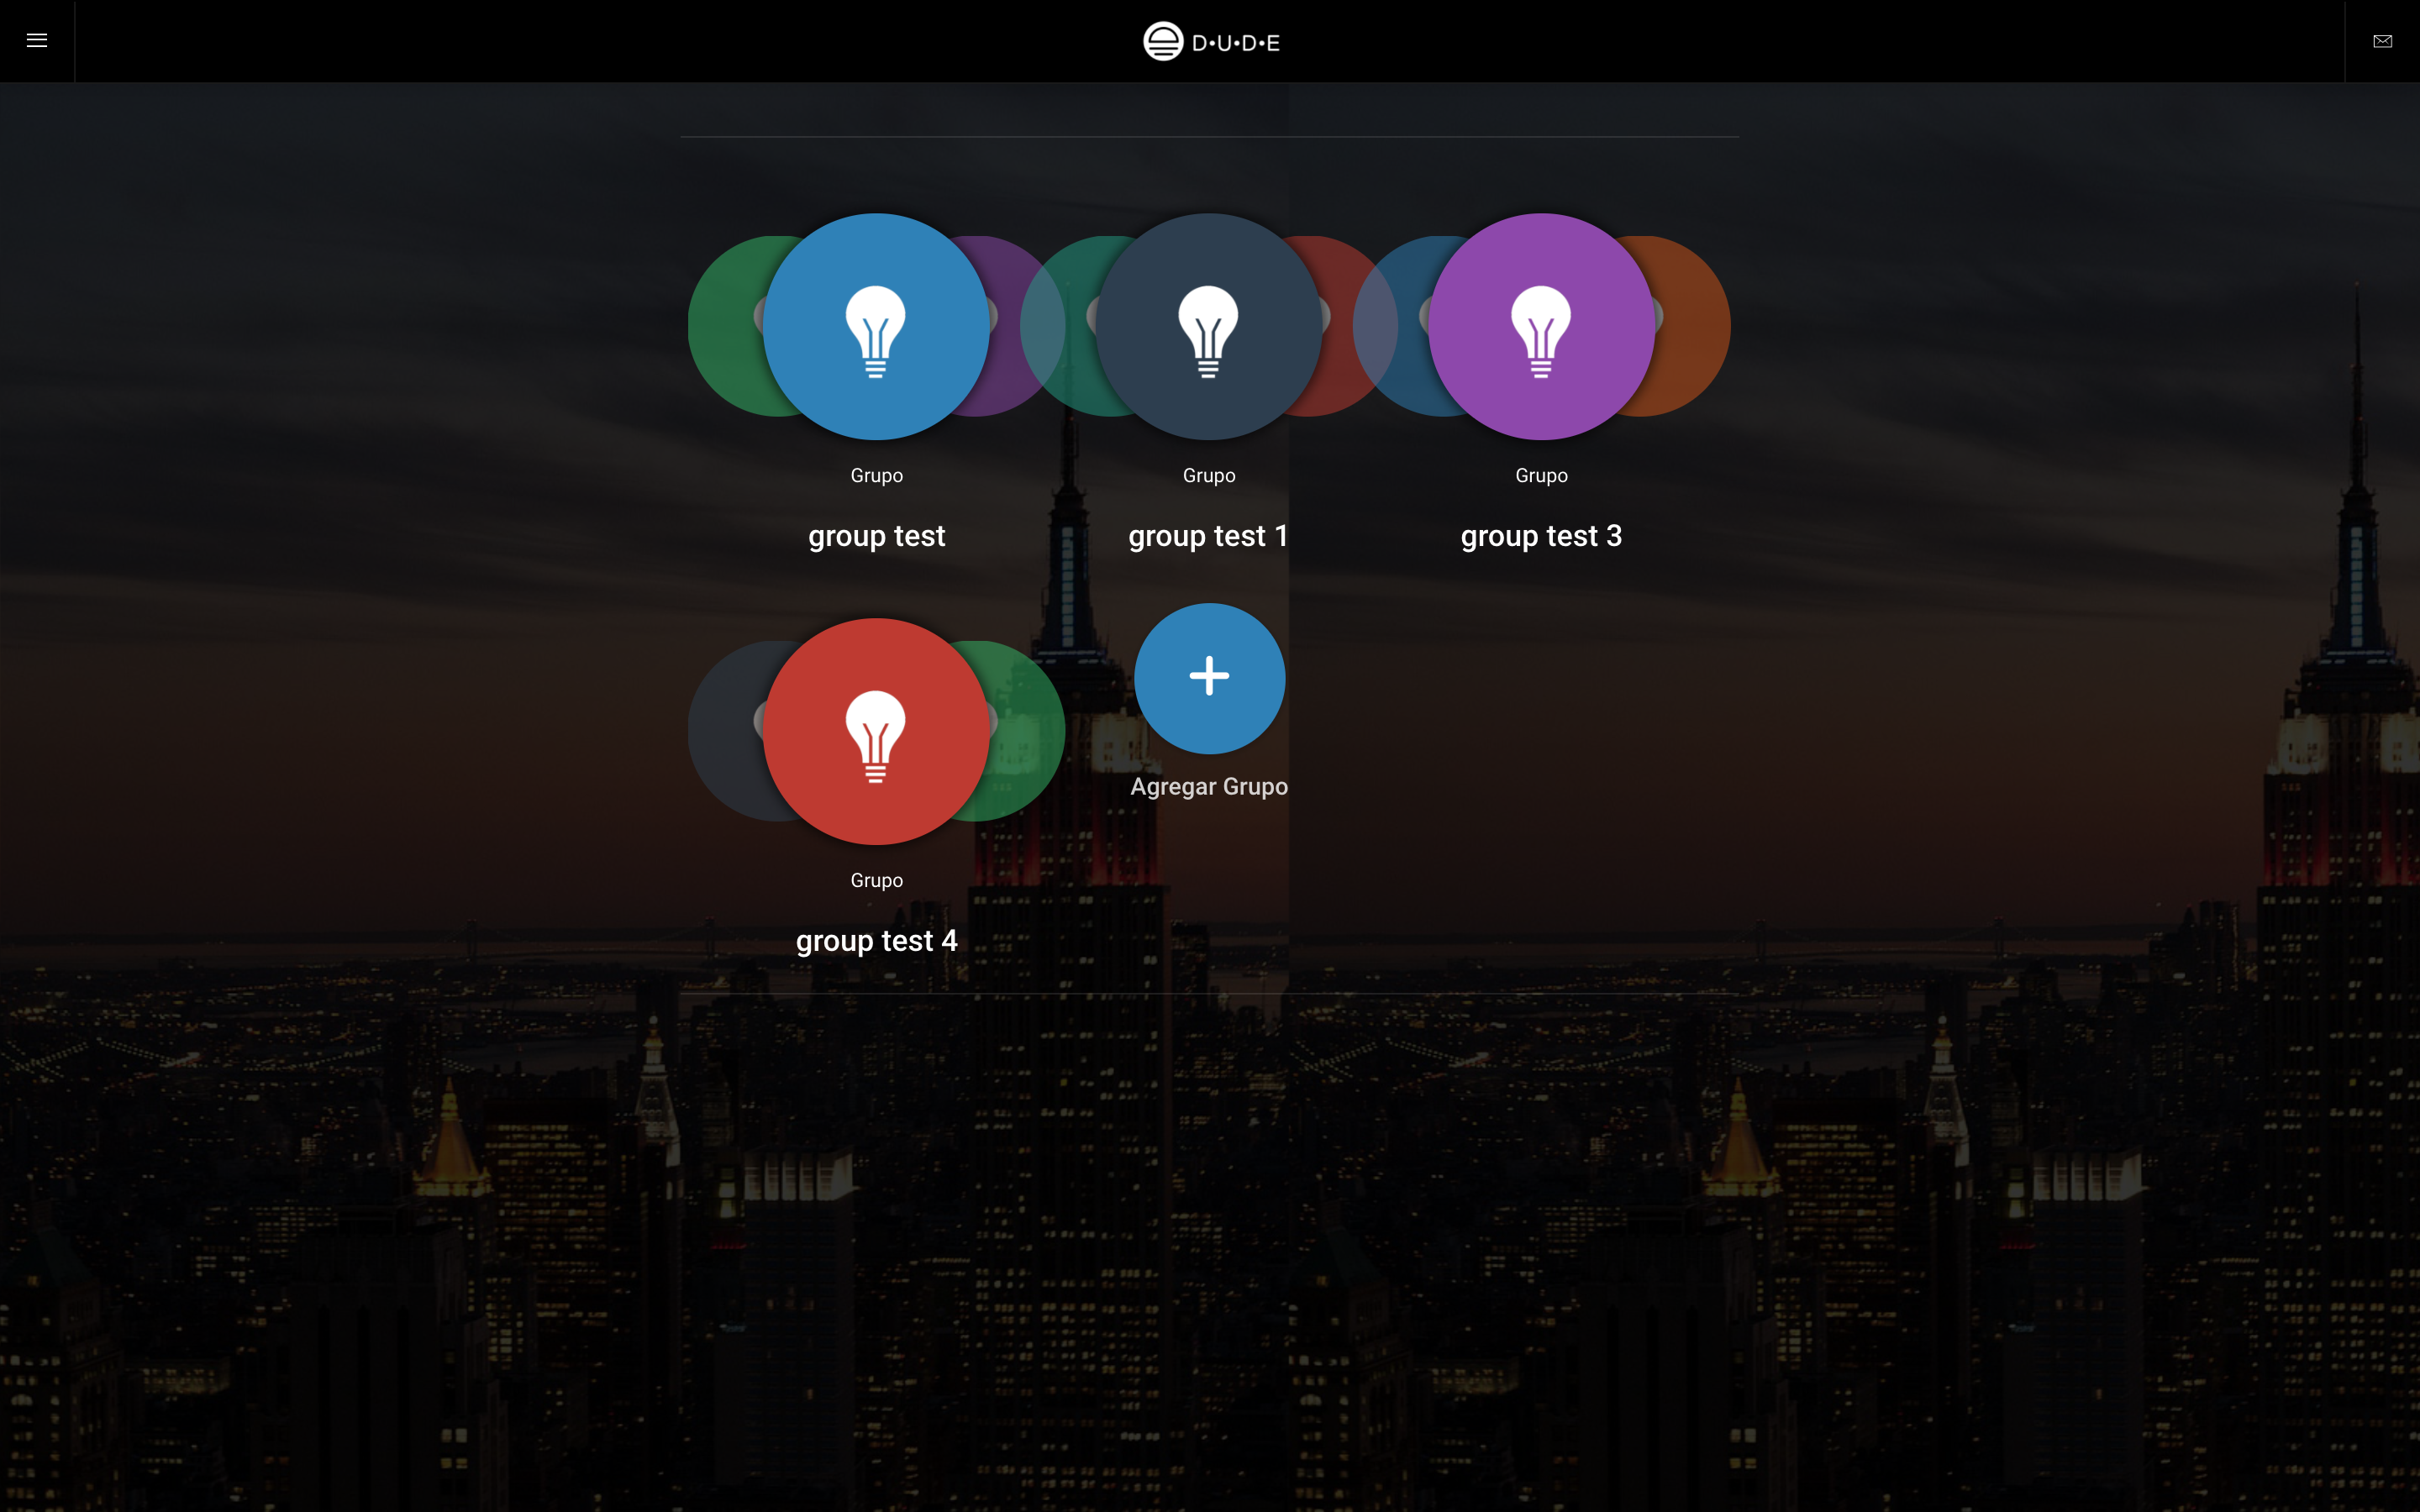
\includegraphics[width=\textwidth, keepaspectratio]{images/app-web-choose-group}
    \caption{\textit{Grupo.}}
    \label{fig:app-web-choose-group}
  \end{subfigure}

\caption{\textit{Vistas de selección.}}
\end{figure}

\textbf{Acciones programadas}\\
La interfaz para agregar una acción cuenta con 3 botones, así como una interfaz gráfica brindada por la librería \lstinline[columns=fixed]{jquery-cron} explicada anteriormente para la elección de la hora, día, mes, año, día de la semana, minuto de cada hora que el usuario puede elegir para programar la acción. En la parte superior aparece el nombre del dispositivo o grupo al que se le quiere aplicar esta acción.~\qref{fig:app-movil-scheduler-device}

Los 3 botones son: apagar, prender, eliminar. Dependiendo de si se eligió dispositivo o grupo, se mandará el id del dispositivo o grupo elegido. Si se selecciona la opción eliminar se eliminan todos los crones para el dispositivo o grupo. Si se elige prender o apagar, se mandará esa acción junto con el cron que traduce la librería que eligió el usuario y el \lstinline[columns=fixed]{id} que se explicó previamente.

\begin{figure}[H]
  \centering
  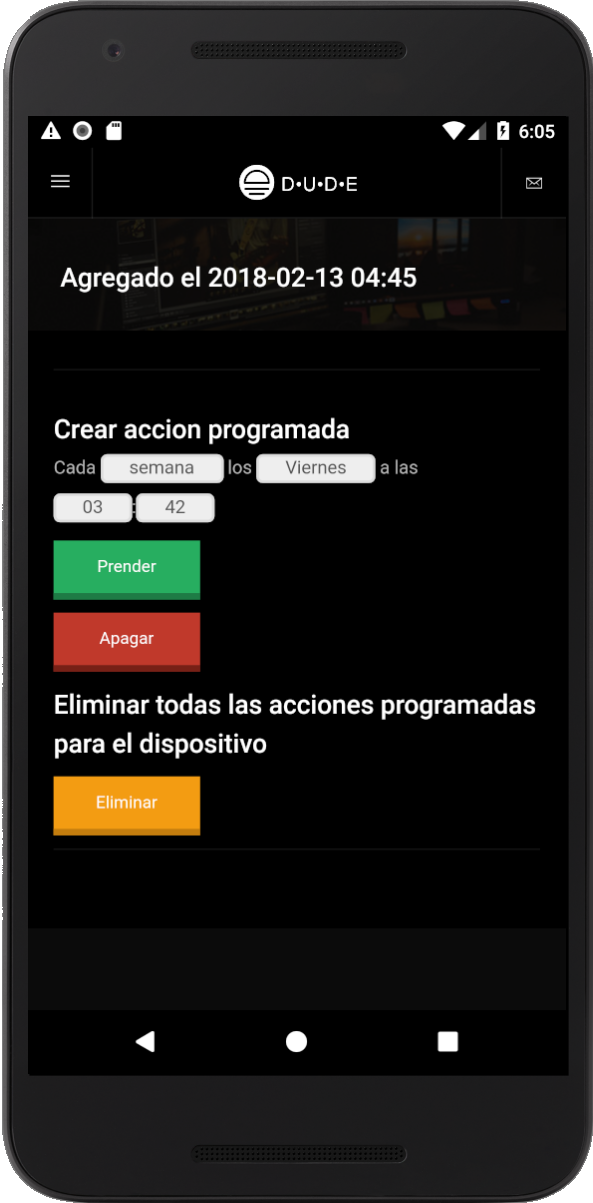
\includegraphics[width=0.2\textwidth, keepaspectratio]{images/app-movil-scheduler-device}
  \caption{\textit{Agregar acción programada.}}
  \label{fig:app-movil-scheduler-device}
\end{figure}


\textbf{Agregar entidad}\\
Esto da la posibilidad de agregar un dispositivo o un grupo.\\
\begin{itemize}
  \item \lstinline[columns=fixed]{Dispositivo}: Para agregar un dispositivo tiene que haber un Sonoff en modo descubrimiento, es decir, un Sonoff que tenga la luz de su led parpadeando. Esto quiere decir que está creando una red llamada \lstinline[columns=fixed]{ConnectAP}. Teniendo esto en cuenta, al seleccionar la pestaña de agregar dispositivo  aparece en pantalla un texto que indica al usuario que se conecte a la red \lstinline[columns=fixed]{ConnectAP}. Cuando este se conecta a esa red, la aplicación lo lleva a la pantalla de inicio dado que que mandaron los datos correctamente a al dispositivo y este queda correctamente agregado.~\qref{fig:app-movil-add-device}
\end{itemize}

\begin{figure}[H]
  \centering
  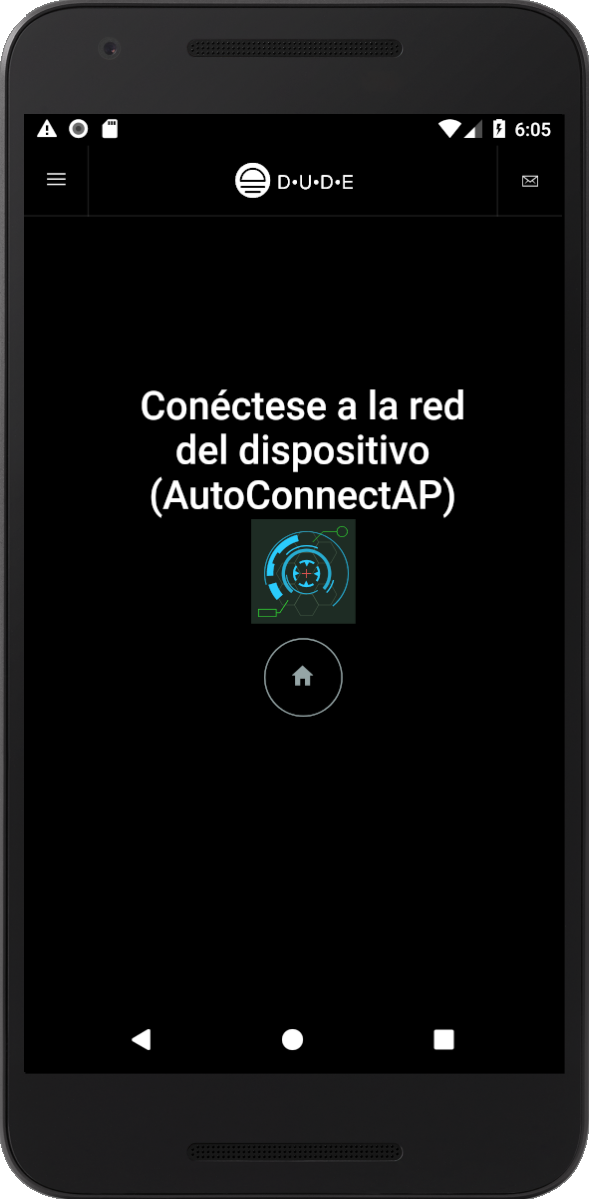
\includegraphics[width=0.2\textwidth, keepaspectratio]{images/app-movil-add-device}
  \caption{\textit{Agregar dispositivo.}}
  \label{fig:app-movil-add-device}
\end{figure}

 \begin{itemize}
  \item \lstinline[columns=fixed]{Grupo}:presenta una interfaz gráfica que lista todos los dispositivos agregados por el usuario, permitiendo seleccionar los que se desea incluir en el grupo y un elegir un nombre. Al texto que introduce el usuario se modifica para evitar problemas. Algunas de las correcciones son: sustituir espacios por uno solo, borra tabs y new lines, impone mayúscula a la primer letra del nombre. Una vez que el usuario presiona el botón confirmar, se envían esos datos al dispositivo central para que los agregue a la base de datos.~\qref{fig:app-movil-edit-group}
\end{itemize}

\begin{figure}[H]
  \centering
  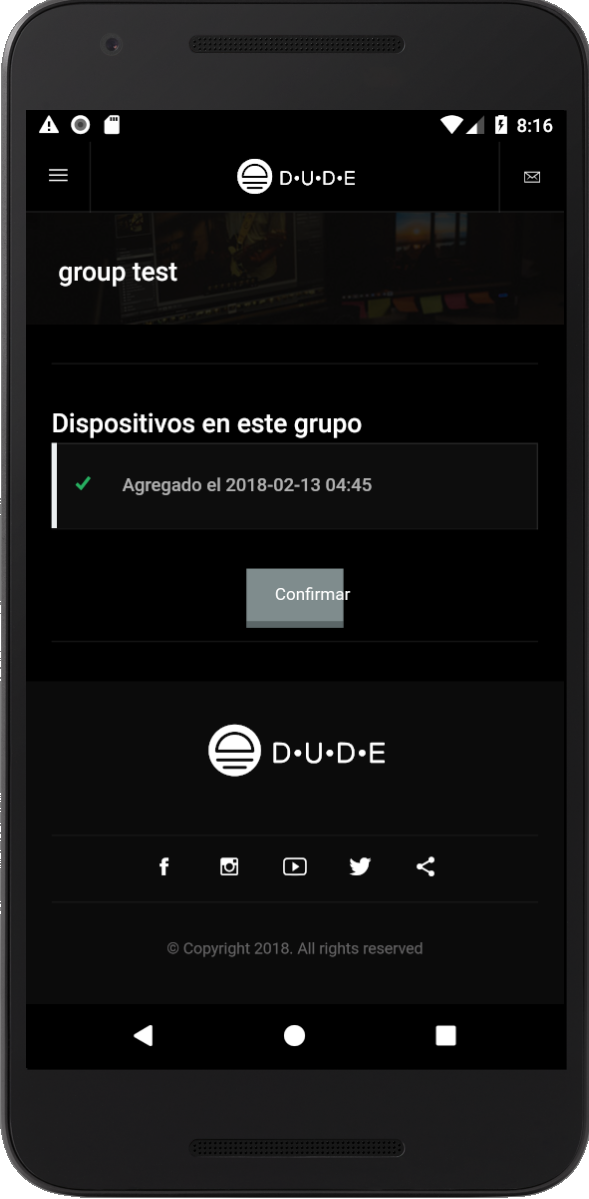
\includegraphics[width=0.2\textwidth, keepaspectratio]{images/app-movil-edit-group}
  \caption{\textit{Agregar grupo.}}
  \label{fig:app-movil-edit-group}
\end{figure}


\textbf{Editar entidad}\\
La opciones que se brindan son editar dispositivo o editar grupo.\\
\begin{itemize}
  \item \lstinline[columns=fixed]{Dispositivo}: lleva a una interfaz con todos los dispositivos registrados y la opción de agregar un dispositivo nuevo~\qref{fig:app-movil-choose-device}.Una vez que se elige uno de ellos, se va a la interfaz de edición de dispositivo. En esta se muestra el nombre del dispositivo, que ser presionado permite la edición del mismo. Se despliegan todos los grupos registrados en la base de datos. Si el dispositivo ya pertenece a alguno de ellos, aparece con un tick a la izquierda. Todos pueden seleccionarse o dejarse de seleccionar según las preferencias del usuario. El botón de confirmar manda los Id de todos los grupos seleccionados para ese dispositivo y el nombre que está escrito en esa interfaz, este cambiado o no. También se manda el \lstinline[columns=fixed]{id} del dispositivo al que se le aplicaron los cambios y se vuelve al menú inicial.~\qref{fig:app-movil-edit-device}
\end{itemize}

\begin{figure}[H]
  \centering
  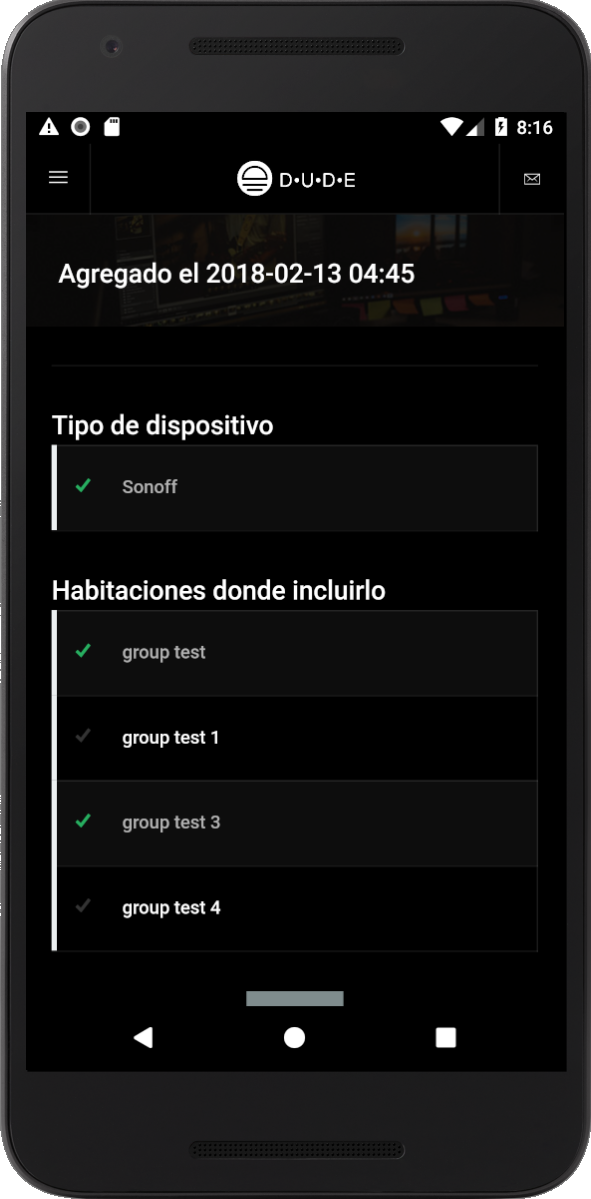
\includegraphics[width=0.2\textwidth, keepaspectratio]{images/app-movil-edit-device}
  \caption{\textit{Editar dispositivo.}}
  \label{fig:app-movil-edit-device}
\end{figure}

\begin{itemize}
  \item \lstinline[columns=fixed]{Grupo}: lleva a una interfaz con todos los grupos registrados además de la opción de agregar un nuevo grupo~\qref{fig:app-web-choose-group}.Una vez elegido el grupo, aparece una interfaz equivalente a la de nuevo grupo. La única diferencia es que en esta interfaz, si hay dispositivos seleccionados previamente para integrar ese grupo, aparecerán con un tick a la izquierda de su nombre en la lista de dispositivos. De forma similar a lo explicado para el editar grupo, al presionar el botón confirmar se manda el \lstinline[columns=fixed]{id} del grupo editado, una lista con los Id de los dispositivos elegidos y el nombre del grupo que aparece en pantalla.~\qref{fig:app-movil-edit-group}
\end{itemize}

\begin{figure}[H]
  \centering
  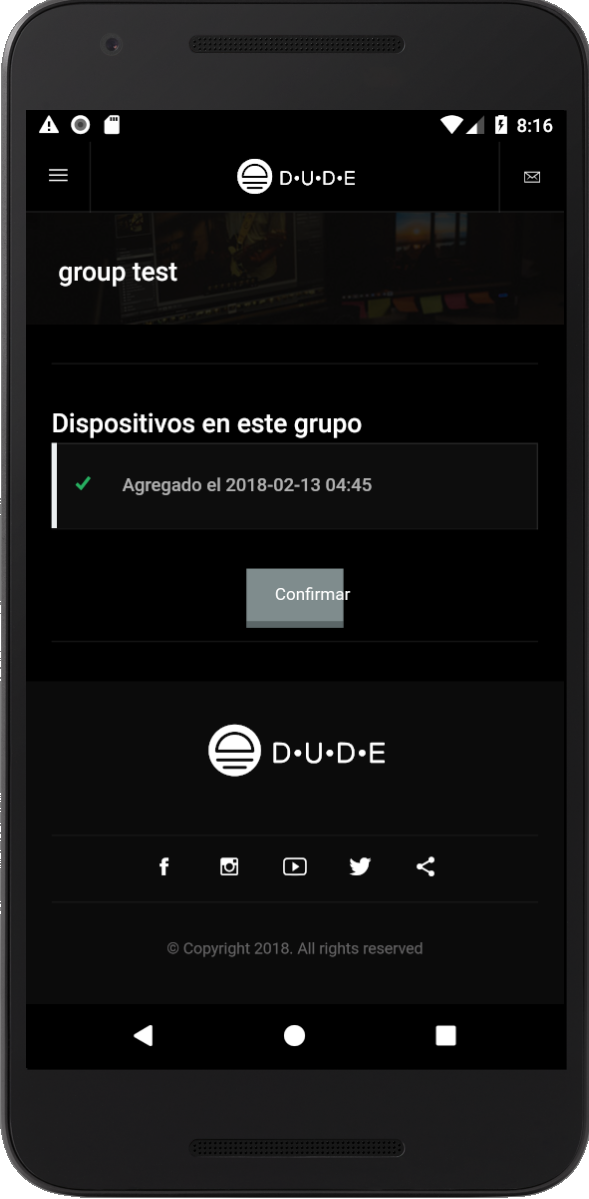
\includegraphics[width=0.2\textwidth, keepaspectratio]{images/app-movil-edit-group}
  \caption{\textit{Editar grupo.}}
  \label{fig:app-movil-edit-group}
\end{figure}

\textbf{Error}\\
En caso de haber un error de conexión con el flask, el usuario verá una pantalla de error que es la siguiente. ~\qref{fig:app-movil-error}

\begin{figure}[H]
  \centering
  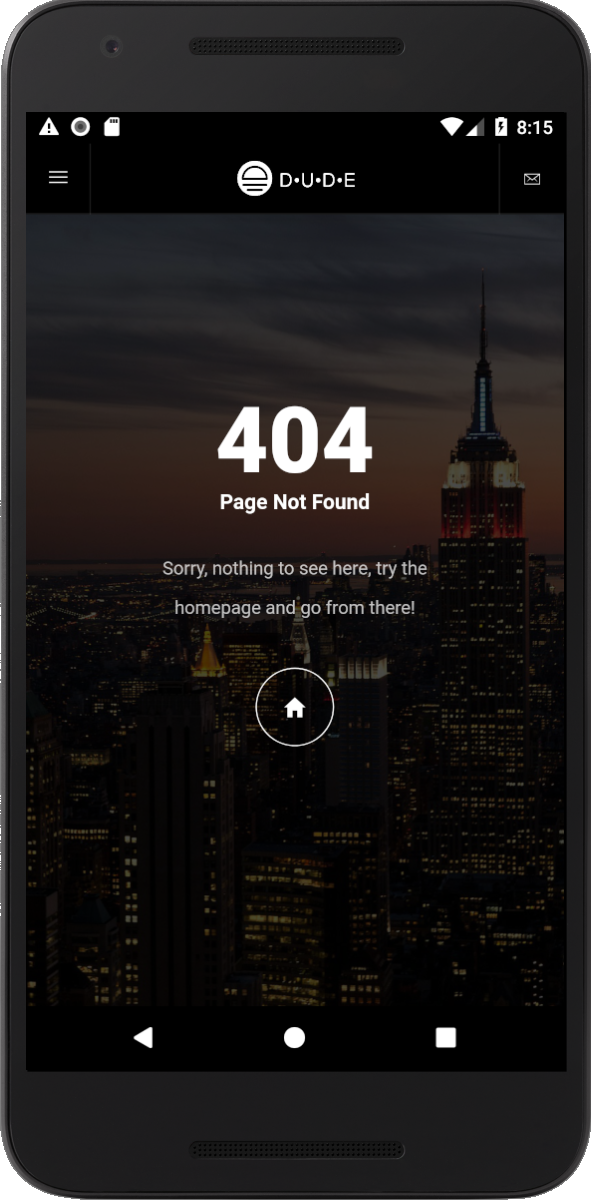
\includegraphics[width=0.2\textwidth, keepaspectratio]{images/app-movil-error}
  \caption{\textit{Pantalla de error.}}
  \label{fig:app-movil-error}
\end{figure}

\subparagraph{Hosting de aplicación web}\mbox{}\mbox{}\\
Para que la aplicación sea accesible y su mantenimiento no sea una sobrecarga, se decidieron utilizar \lstinline[columns=fixed]{AWS} (Amazon Web Services) donde se levantó una máquina virtual con \lstinline[columns=fixed]{EC2} que sirve un \lstinline[columns=fixed]{Apache HTTP Server}.

\textbf{Amazon EC2}\\
Para crear una máquina virtual, primero se necesita elegir que sistema operativo. En este proyecto, como solo se debe mostrar un prototipo, se eligió una de las opciones gratis que brinda AWS con Ubuntu de arranque. Se optó por Ubuntu dado que se tenía experiencia instalado servidores Apache ahí. \qref{fig:AWS1}

\begin{figure}[H]
  \centering
  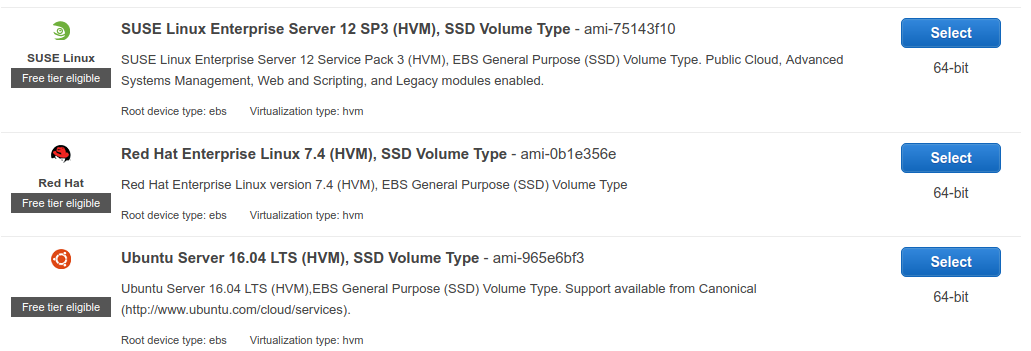
\includegraphics[width=\textwidth, keepaspectratio]{images/AWS1}
  \caption{\textit{Elección de SO.}}
  \label{fig:AWS1}
\end{figure}

Luego de elegir el sistema operativo, hay que elegir cuanta \lstinline[columns=fixed]{RAM}, procesador, característica de red se quiere tener. En este caso, solo había una opción gratis  y que a su vez tenía todo lo que se necesitaba para el servidor. Por lo que se eligió esa. \qref{fig:AWS2}

\begin{figure}[H]
  \centering
  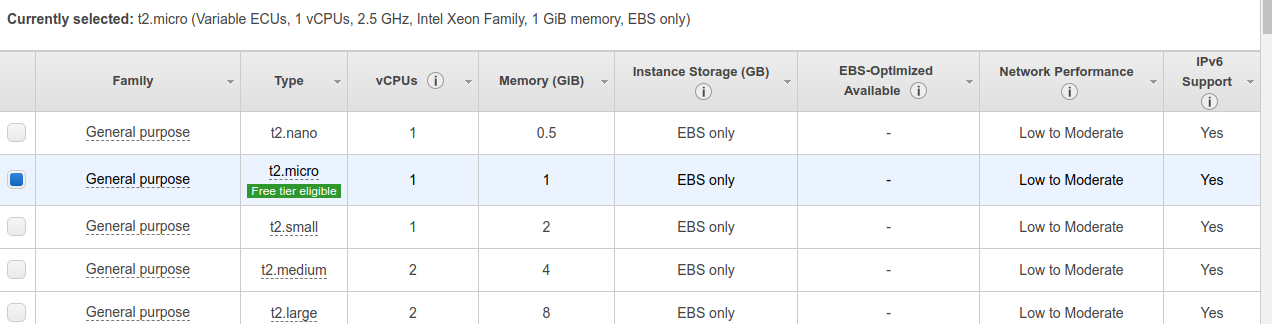
\includegraphics[width=\textwidth, keepaspectratio]{images/AWS2}
  \caption{\textit{Elección de máquina virtual.}}
  \label{fig:AWS2}
\end{figure}

Finalmente se le debe asignar un grupo de seguridad a esa instancia como se ve a continuación. \qref{fig:AWS3}

\begin{figure}[H]
  \centering
  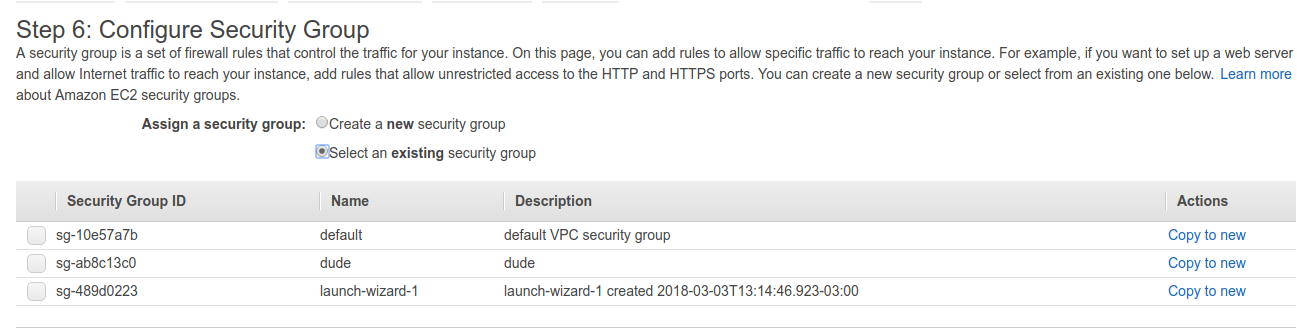
\includegraphics[width=\textwidth, keepaspectratio]{images/AWS3}
  \caption{\textit{Elección de grupo de seguridad.}}
  \label{fig:AWS3}
\end{figure}

Por lo tanto, antes de esto se creó un grupo de seguridad acorde para este servicio. Se habilitó el ping tanto como las conexiones \lstinline[columns=fixed]{TCP} en el puerto \lstinline[columns=fixed]{80}. El \lstinline[columns=fixed]{SSH} en el puerto \lstinline[columns=fixed]{22} ya estaba habilitado previamente. Todo el tráfico saliente ya está habilitado por defecto. \qref{fig:AWS4}

\begin{figure}[H]
  \centering
  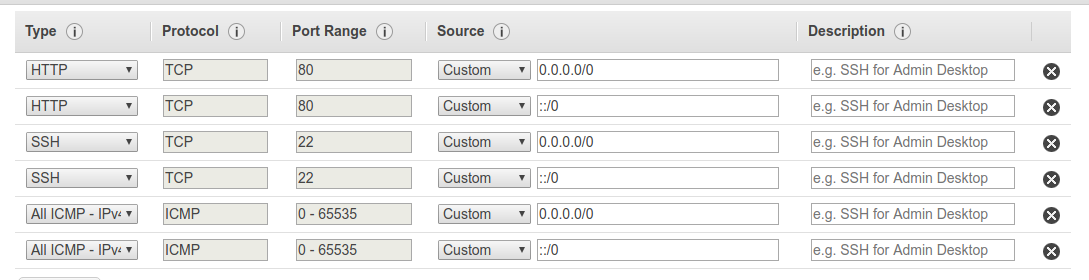
\includegraphics[width=\textwidth, keepaspectratio]{images/AWS4}
  \caption{\textit{Creación de grupo de seguridad.}}
  \label{fig:AWS4}
\end{figure}

Luego de crear la instancia, \lstinline[columns=fixed]{AWS} da al usuario una llave para que pueda conectarse con el servidor en cuestión. La llave se puede elegir de otra ya existente o crear una nueva. El usuario guarda su llave privada, mientras que la instancia que acaba de crear se queda con la llave pública. \qref{fig:AWS5}

\begin{figure}[H]
  \centering
  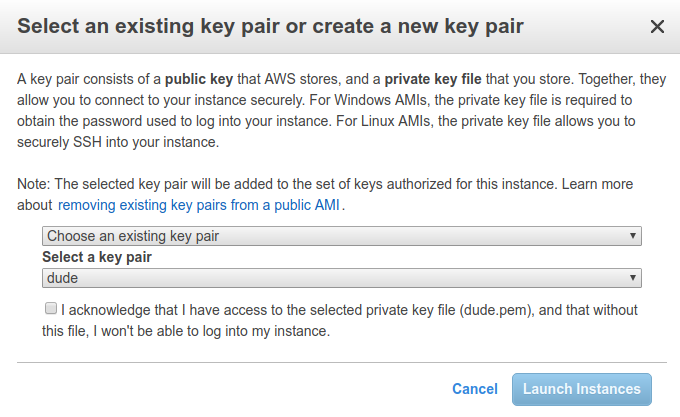
\includegraphics[width=\textwidth, keepaspectratio]{images/AWS5}
  \caption{\textit{Elección de llave.}}
  \label{fig:AWS5}
\end{figure}

Terminado esto queda la máquina virtual corriendo. Hay un panel web que permite ver el estado de la misma, su IP su DNS público como se ve a continuación. \qref{fig:AWS6}

\begin{figure}[H]
  \centering
  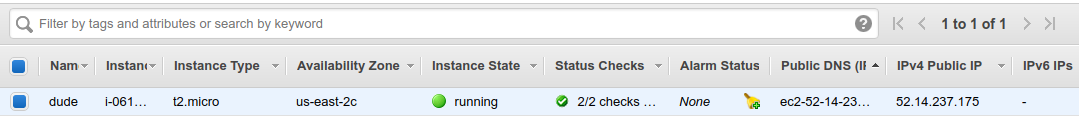
\includegraphics[width=\textwidth, keepaspectratio]{images/AWS6}
  \caption{\textit{Panel informativo.}}
  \label{fig:AWS6}
\end{figure}

\textbf{Apache HTTP Server}\\
Primero se instala Apache mediante el gestor de paquetes de Ubuntu de la siguiente manera: 
\begin{lstlisting}[language=bash]
apt-get install apache2
\end{lstlisting}
Luego, todo el código generado por Phonegap para la plataforma de navegador se puso en la carpeta \lstinline[columns=fixed]{/var/www/html/dude}. Asimismo, se necesita que todos los llamados que van al puerto 80 sea atendido por el servidor Apache y este llame a los archivos en \lstinline[columns=fixed]{/var/www/html/dude}. 

Para lograr esto en el archivo ports.conf se tiene que configurar que apache escuche en el puerto \lstinline[columns=fixed]{80} (lo cual se hace por defecto) de la siguiente manera:

Listen 80

Una vez que se escucha lo que llega a ese puerto, hay que direccionar el tráfico a la carpeta \lstinline[columns=fixed]{/var/www/html/dude}. Para esto, en \lstinline[columns=fixed]{sites-available} hay que modificar el archivo por defecto de servidor para que el tráfico que llega a ese puerto se direccione a \lstinline[columns=fixed]{/var/www/html/dude} y no a \lstinline[columns=fixed]{/var/www/html}, como hace por defecto. El archivo por defecto modificado es \lstinline[columns=fixed]{000-default.conf}.

\begin{lstlisting}[language=bash]
<VirtualHost *:80>
        ServerAdmin webmaster@localhost
        DocumentRoot /var/www/html/dude

        ErrorLog ${APACHE_LOG_DIR}/error.log
        CustomLog ${APACHE_LOG_DIR}/access.log combined
</VirtualHost>
\end{lstlisting}

Finalmente, hay que habilitar ese archivo y reiniciar el servidor apache 

\begin{lstlisting}[language=bash]
sudo a2ensite 000-default.conf
sudo service apache2 restart
\end{lstlisting}



\subsubsection{Mycroft}

Se desarrollaron skills para el asistente virtual \lstinline[columns=fixed]{Mycroft}~\cite{Mycroft} como una de las interfaces que permitirán al usuario interactuar con el sistema, pero a diferencia de las aplicaciones móvil y web, esta interfaz tiene funcionalidades más básicas, ya que la interfaz por vos no resulta cómoda para acciones complejas, como agregar dispositivos o modificar los mismos.
Mycroft cuenta con dos versiones en la actualidad, una para Linux y otra pensada específicamente para Raspberry Pi, llamado Picroft. La segunda contiene a la implementación de Linux además de otros archivos y configuraciones necesarios para lograr la compatibilidad de Mycroft con esta plataforma y sus drivers.
Debido a problemas en actualizaciones en los servidores de Mycroft y debido a que el proyecto Picroft se ha enfocado más en la compatibilidad con los productos Mark 1 y Mark 2 (hardware compuesto por Raspberry Pi con micrófonos y parlantes montados), ocurrieron errores con las configuraciones de Raspberry's más generales.
Siendo imposible la instalación correcta y funcional de Picroft, se consultó en foros de la comunidad y nos pusimos en contacto con desarrolladores del proyecto, aportando logs de nuestras instalaciones para ayudar a descubrir y solucionar el problema (~\cite{Topic1}, ~\cite{Topic2}).
A pesar de su apoyo no se logró el cometido, siendo que descubrimos que era un problema general y contamos con nuestros topics entre los más comentados y vistos a la semana de realizar la publicación.
Luego de estos intentos se decidió que se debía optar por una alternativa, considerando las herramientas de Google y Amazon para esto, a pesar de que se alejaban del perfil open source y sin monetización de datos del cliente. Por estas razones y sumada la confianza en el equipo de Mycroft y en la comunidad para que se resuelvan los problemas en Picroft, se decidió por desarrollar los skills con Mycroft instalado en Linux, ya que cuando eventualmente Picroft vuelva a un estado estable, se pueden utilizar los mismos skills.

Debido a los contratiempos se desarrollaron únicamente skills de cambio de estado de luces, cuyos llamados son:
\begin{itemize}
  \item Prender luces:
    \begin{itemize}
      \item turn on the lights
      \item turn the lights on
      \item make it shine
      \item light me up
    \end{itemize}
  \item Apagar luces:
    \begin{itemize}
      \item turn off the lights
      \item turn the lights off
      \item darkness please
    \end{itemize}
\end{itemize}


Para el desarrollo y entendimiento de la implementación de skills se siguió la guía introductoria brindada por el equipo de \lstinline[columns=fixed]{Mycroft}~\cite{GuiaMycroft}.
La estructura básica de un skill es:
\begin{itemize}
  \item Directorios

  \begin{itemize}
    \item dialog: contiene una carpeta por idioma, que a su vez contienen los archivos con frases de respuesta para skills, de los que Mycroft elige de forma aleatoria dentro de un archivo.
    \item test: contiene archivos para realizar tests de intents.
    \item vocab: similar al directorio dialog, solo que los archivos contienen frases que determinan la intención de utilizar un skill.
  \end{itemize}

  \item Archivos
  \begin{itemize}
    \item \_\_init\_\_.py: Este es el cuerpo principal del skill, donde se definen los intents y las definiciones handler, que contienen la lógica de la función a ejecutar.
    \item LICENSE: Archivo que determina el tipo de licencia bajo la que se rige el skill.
    \item README.md: Archivo que explica la utilización del skill.
    \item requirements.sh y requirements.txt: Archivos que definen las dependencias necesarias para el funcionamiento de los skills.

  \end{itemize}
\end{itemize}

\subsection{Aportes a librerías de terceros}

A medida que se avanzó en el proyecto se encontraron problemas u oportunidades de mejora en algunas librerías que fueron utilizadas para llevar a cabo el proyecto. Esto generó que, a pesar que no fuera un objetivo desde el comienzo, se mejoró o ayudó a mejorar estas librerías.

\subsubsection{ESP8266MQTTMesh}

Se encontró un problema que provocaba que no se pudiera conectar a la red MQTT el dispositivo si no se conseguían los datos como el nombre de red y contraseña desde un archivo de texto que se cargaba con el código. De esta manera, estos parámetros no podían ser guardados en los SPIFFS para conseguirlos luego. Esto se reportó en el issue ~\cite{Topic2} y se consiguió una rápida respuesta de parte del programador a cargo. Esto llevó a que la librería ahora pueda integrarse con proyectos como WiFiManager, que brindan una conexión con el ESP para que se pueda elegir la SSID a la cual conectarse y la contraseña.https://github.com/PhracturedBlue/ESP8266MQTTMesh/issues/29  Esto fue implementado por en este proyecto e tesis y casualmente otra persona lo solicitó https://github.com/PhracturedBlue/ESP8266MQTTMesh/issues/38. Por este motivo, al terminar el proyecto se va a agregar un código de ejemplo a la librería  ESP8266MQTTMesh para que otras personas puedan integrar ambas librerías, haciéndola una opción muy atractiva. 

Finalmente, también se ayudó a mejorar la librería desde el aspecto del debuggeo. Se tuvo un problema cuya causa fue una elección errónea de versión de plataforma. A partir de esto, el programador encargado del proyecto agregó código que no deja compilar si la elección de la plaforma no es la adecuada. De esta forma se ahorró horas de debuggeo de issues cuyo problema no sea el código en sí. https://github.com/PhracturedBlue/ESP8266MQTTMesh/issues/19 

\subsubsection{jquery-cron}

Se creó un fork de la librería con la traducción al español de la misma. Este fork es visible para todo el mundo. https://github.com/alexiszecharies/jquery-cron https://github.com/shawnchin/jquery-cron/issues/33 

\subsubsection{WiFiManager}

Se ayudó en el testeo de un fork en estado de development de esta librería. Se encontró un error que luego fue corregido por el encargado de ese fork. https://github.com/tzapu/WiFiManager/issues/472 A su vez, se modificó el código fuente para cumplir con uno de los requisitos del proyecto y se dejó constancia de cómo se hizo para lograr esto en ese issue.
